\documentclass[12pt]{ucthesis}

% This needs to be added before hyperref
\usepackage[papersize={8.5in,11in},inner=1.5in,outer=1.25in,top=1.25in,bottom=1.25in]{geometry}

\usepackage{fixltx2e}
\usepackage{url}
\usepackage{amsmath, amsthm, amssymb}
\usepackage{color}
\usepackage{xspace}
\usepackage{verbatim}
\usepackage{graphicx}
\usepackage{psfrag}
\usepackage{pbox}
\usepackage{epstopdf}
\usepackage{textcomp} % For copyright symbol
\DeclareGraphicsExtensions{.pdf,.eps,.png,.jpg}
\usepackage[font=singlespacing]{subcaption}
\captionsetup[table]{labelfont=bf,font=singlespacing}
\captionsetup[figure]{labelfont=bf,font=singlespacing}
\captionsetup[subfigure]{labelfont=bf,font=singlespacing}
\usepackage[titletoc,title]{appendix}
\usepackage{tabularx}
\usepackage{rotating}
\usepackage{hyperref} % Turns all internal references into links to pages within the document
\hypersetup{pdfborder={0 0 0}} % removes red box from links

\usepackage{lmodern} % Use the Latin Modern font
\usepackage[T1]{fontenc} % Use a modern font encoding

\makeatletter % Hack to get setspace working properly
\let\@currsize\normalsize
\makeatother
\usepackage{setspace}% http://ctan.org/pkg/setspace


% more packages
\usepackage{bibentry} % to print reference in plaintext. used in chap. ack.
\usepackage[capitalise]{cleveref}
\usepackage{mathtools} % \coloneqq
\usepackage{siunitx} % needed for printing a scientific number \num{e-10}
\usepackage{bm}

% Set default spacing to double (yes, it should be 1.6 here...)
\linespread{1.6}

% I will save your typings

% colors
\newcommand{\red}[1]{\color{red} #1 \color{black}}
\newcommand{\blue}[1]{\color{blue} #1 \color{black}}
\newcommand{\green}[1]{\color{green} #1 \color{black}}
% notes in colors
\newcommand{\noteb}[1]{\textcolor{blue}{{\bf#1}}}
\newcommand{\noter}[1]{\textcolor{red}{{\bf#1}}}

% \bf things
\newcommand{\bA}{\mathbf{A}}
\newcommand{\bB}{\mathbf{B}}
\newcommand{\bC}{\mathbf{C}}
\newcommand{\bD}{\mathbf{D}}
\newcommand{\bF}{\mathbf{F}}
\newcommand{\bG}{\mathbf{G}}
\newcommand{\bH}{\mathbf{H}}
\newcommand{\bI}{\mathbf{I}}
\newcommand{\bJ}{\mathbf{J}}
\newcommand{\bK}{\mathbf{K}}
\newcommand{\bk}{\mathbf{k}}
\newcommand{\bL}{\mathbf{L}}
\newcommand{\bM}{\mathbf{M}}
\newcommand{\bP}{\mathbf{P}}
\newcommand{\bQ}{\mathbf{Q}}
\newcommand{\bR}{\mathbf{R}}
\newcommand{\bT}{\mathbf{T}}
\newcommand{\bU}{\mathbf{U}}
\newcommand{\bV}{\mathbf{V}}
\newcommand{\bW}{\mathbf{W}}
\newcommand{\bw}{\mathbf{w}}
\newcommand{\bX}{\mathbf{X}}
\newcommand{\bY}{\mathbf{Y}}
\newcommand{\Z}{\mathbb{Z}}
%
\newcommand{\ba}{\mathbf{a}}
\newcommand{\bb}{\mathbf{b}}
\newcommand{\bc}{\mathbf{c}}
\newcommand{\be}{\mathbf{e}}
\newcommand{\bff}{\mathbf{f}}      % avoid \bf command
\newcommand{\bg}{\mathbf{g}}
\newcommand{\bh}{\mathbf{h}}
\newcommand{\bq}{\mathbf{q}}
\newcommand{\br}{\mathbf{r}}
\newcommand{\bl}{\mathbf{\ell}}
\newcommand{\buu}{\mathbf{u}}
\newcommand{\bvv}{\mathbf{v}}
\newcommand{\bx}{\mathbf{x}}
\newcommand{\by}{\mathbf{y}}
\newcommand{\bz}{\mathbf{z}}
%
\newcommand{\bmu}{\bm{\mu}}     % mathbf{mu} is not working, 
%
\newcommand{\bfone}{\mathbf{1}}
\newcommand{\bfzero}{\mathbf{0}}
%
\newcommand{\bfeta}{\mbox{\boldmath$\eta$}}
\newcommand{\bfPsi}{\mbox{\boldmath$\Psi$}}
\newcommand{\bfOmega}{\mbox{\boldmath$\Omega$}}
\newcommand{\bfPhi}{\mbox{\boldmath$\Phi$}}

% half is not 1/2
\newcommand{\half}{\frac{1}{2}}
% d is not delta
\newcommand{\dt}{\Delta t}
\newcommand{\dx}{\Delta x}
\newcommand{\dy}{\Delta y}
\newcommand{\dz}{\Delta z}

% partial derivatives!
% \newcommand{\pd}[2]{\frac{\partial #1}{\partial #2}}
% \newcommand{\pdd}[2]{\frac{\partial^{2} #1}{\partial #2^{2}}}
% \newcommand{\pddd}[2]{\frac{\partial^{3} #1}{\partial #2^{3}}}

\newcommand{\pd}[2]{\partial_{#2} #1}
\newcommand{\pdd}[2]{\partial^{2}_{#2} #1}
\newcommand{\pddd}[2]{\partial^{3}_{#2} #1}

% vector is bold
\renewcommand{\vec}[1]{\mathbf{#1}}
\newcommand{\hvec}[1]{\hat{\mathbf{#1}}}

% discrete indices with halves
\newcommand{\nph}{{n+\frac{1}{2}}}
\newcommand{\nmh}{{n-\frac{1}{2}}}
\newcommand{\iph}{{i+\frac{1}{2}}}
\newcommand{\imh}{{i-\frac{1}{2}}}
\newcommand{\jph}{{j+\frac{1}{2}}}
\newcommand{\jmh}{{j-\frac{1}{2}}}
\newcommand{\kph}{{k+\frac{1}{2}}}
\newcommand{\kmh}{{k-\frac{1}{2}}}

% semi-colon
\newcommand{\scolon}{\,;\,}

% declare argmin and argmax
\DeclareMathOperator*{\argmax}{arg\,max}
\DeclareMathOperator*{\argmin}{arg\,min}

% used for sfPIF
\newcommand{\Div}{\nabla^{f}}

% ERF
\newcommand{\erf}[1]{\operatorname{erf} \left [ #1 \right ]}


\begin{document}

\title{A Fast and Portable High-Order Temporal Solver for Computational Fluid Dynamics}
\author{Youngjun Lee}
\degreeyear{2021}
\degreemonth{September}
\degree{DOCTOR OF PHILOSOPHY}
\chair{Professor Dongwook Lee}
\committeememberone{Professor Nicholas Brummell}
\committeemembertwo{Professor Hongyun Wang}
%\committeememberthree{Professor 4} % Uncomment if you have 4 committee members. Also change the next line to `\numberofmembers{4}`
\numberofmembers{3}
\deanlineone{Peter Biehl}
\deanlinetwo{Vice Provost and Dean of Graduate Studies}
\deanlinethree{}
\field{Applied Mathematics and Statistics}
\campus{Santa Cruz}

\begin{frontmatter}
\maketitle

\copyrightpage

\tableofcontents

\listoffigures

\listoftables

%%%%%%%%%%%%
% Abstract %
%%%%%%%%%%%%
\begin{abstract}
The recent advent of high-performance computing hardware enables large-scale, multi-physics simulation that provides accurate physical pictures in various fields of study. In order to utilize the high-performance computing system more efficiently, the high-order numerical approximations have become one of the central themes in computational fluid dynamics (CFD) due to their potential in achieving highly accurate predictions in a limited memory capacity.

The single-stage or single-step high-order temporal discretizations have shown great promise in delivering high-order temporal accuracy in fast performance. Fundamentally, the single-stage time integrators are based on a Taylor series in the time domain. Although its high performance, the single-stage time integrators are less attractive and less flexible compared to the multi-stage methods due to the complexities in calculating the coefficient of time-Taylor expansion, which usually demands the flux Jacobians and Hessians.

This dissertation develops a new single-stage high-order temporal integrator under finite difference discretization. The proposed high-order temporal method is based on the Lax-Wendroff type time discretization, with an algorithmic extension that provides the system independence property. The new approach, called system-free (SF) method, furnishes ease of implementation as well as portability and flexibility of the single-stage time integration method while maintaining the accuracy and stability of the numerical solution.

\end{abstract}

%%%%%%%%%%%%%%%
% Dedications %
%%%%%%%%%%%%%%%
\begin{dedication}
\vspace*{\fill}
\begin{center}
    To my love, \\ Hyunkyung
\end{center}
\vspace*{\fill}
\end{dedication}

%%%%%%%%%%%%%%%%%%%%
% Acknowledgements %
%%%%%%%%%%%%%%%%%%%%
\begin{acknowledgements}
All the research works presented in this dissertation would not have been possible without the guidance and support of my advisor, Dongwook Lee. Foremostly, I would like to thank Dongwook Lee for his endless support and advice, steering me to the world of numerical methods.

I was very fortunate to participate in the research project at Argonne National Laboratory, which supports the later part of my graduate career. I would like to thank Jeffrey Dooling and Carlo Graziani for giving me an opportunity to join the research project as a visiting graduate student at Argonne National Laboratory.

I also wish to express my gratitude to my Ph.D. committee members, Nicholas Brummell and Hongyun Wang, for giving me many constructive comments and feedback that have improved the dissertation.

Of course, none of what I achieved during my Ph.D. journey would be possible without the love and support of my family, for which I am eternally grateful. 

The text of this dissertation includes reprints of the following previously published material:
\begin{itemize}
    \item Youngjun Lee and Dongwook Lee. A single-step third-order temporal discretization with jacobian-free and hessian-free formulations for finite difference methods. \textit{Journal of Computational Physics}, 427:110063, 2021.
    \item Youngjun Lee, Dongwook Lee, and Adam Reyes. A recursive system-free single-step temporal discretization method for finite difference methods. \textit{Journal of Computational Physics: X}, 12:100098, 2021.
\end{itemize}
The primary co-author Dongwook Lee listed in these publications directed and supervised the research which forms the basis for this dissertation.

I acknowledge the use of the lux supercomputer at UC Santa Cruz, funded by NSF MRI grant AST 1828315.

\end{acknowledgements}

\end{frontmatter}


% lets input actual works
\label{ch:introduction}

\chapter{Discretization Methods}\label{chap:discrete_methods}

This dissertation interests in solving the general conservation laws of hyperbolic PDEs,
predicting numerical solutions with high-order accuracy.
This chapter introduces two general ways to discretize the Euler equations,
which will be of particular interest in this dissertation.

\section{Euler Equations}\label{sec:euler_eqns}

In three dimensions, the conservation laws may be written as,
\begin{equation}\label{eq:gov}
    \partial_{t} \bU + \nabla \cdot \mathcal{F}(\bU)
    = \partial_{t} \bU + \partial_{x} \bF (\bU) + \partial_{y} \bG (\bU) + \partial_{z} \bH (\bU) = 0,
\end{equation}
where \( \bU \) is a vector of conserved variables and
\( \mathcal{F} = {(\bF (\bU), \bG (\bU), \bH (\bU))}^{T} \) is the flux function
in the \( x \), \( y \), and \( z \) directions.
The conservation law is considered hyperbolic
if the flux Jacobian has only real eigenvalues and is diagonalizable. Thus,
\begin{equation}\label{eq:hyperbolic}
    \bA = \partial_{\bU} \bF = \bR \mathbf{\Lambda} \bL,
\end{equation}
where \( \bA \) is the flux Jacobian in \( x \)-direction,
\( \mathbf{\Lambda} \) is a diagonal matrix with real eigenvalues, and
\( \bL \) and \( \bR \) are corresponding left and right eigenvectors.

This dissertation focuses on solving Euler equations, which govern
compressible, adiabatic inviscid flow.
In the Euler equations, the conserved variables and the flux functions are defined as,
\begin{equation}\label{eq:euler-3d}
    \bU = \begin{bmatrix}
        \rho \\
        \rho u \\
        \rho v \\
        \rho w \\
        E
    \end{bmatrix},\;
    \bF (\bU) = \begin{bmatrix}
        \rho u \\
        \rho u^{2} + p \\
        \rho u v \\
        \rho u w \\
        u \left( E + p \right)
    \end{bmatrix},\;
    \bG (\bU) = \begin{bmatrix}
        \rho v \\
        \rho u v \\
        \rho v^{2} + p \\
        \rho v w \\
        v \left( E + p \right)
    \end{bmatrix},\;
    \bH (\bU) = \begin{bmatrix}
        \rho w \\
        \rho u w \\
        \rho v w \\
        \rho w^{2} + p \\
        w \left( E + p \right)
    \end{bmatrix}.
\end{equation}
In the above equations, \( \rho \) is the density,
\( \mathbf{u} = {(u, v, w)}^{T} \) is the velocity,
\( E \) is the total energy, and \( p \) is the pressure of the fluid.
\( E \), the total energy of the fluid represents the
sum of internal and kinetic energy,
\begin{equation}\label{eq:total_E}
    E = \epsilon + \frac{1}{2} \rho \mathbf{u}^{2},
\end{equation}
where the internal energy of the fluid, \( \epsilon \), obeys the equation of state. (EOS)
This dissertation uses the ideal gas law:
\begin{equation}\label{eq:ideal_eos}
    \epsilon = \frac{p}{\gamma - 1},
\end{equation}
where \( \gamma \) is the specific heat ratio.

In the following, this dissertation uses the Euler equation as an example
of the conserved hyperbolic system.
However, numerical methods presented in this dissertation are valid for any system
of the form of~\cref{eq:gov}. Magnetohydrodynamics (MHD) equations, for example,
the general numerical strategies will be nearly identical to the Euler equations
except for the solenoidal constraint of the magnetic field. (\( \nabla \cdot \bB = 0 \))
Thus, the high-order methods presented in this dissertation can be applied to the MHD simulation code easily.


\section{Finite Volume Method}\label{sec:fvm}

The popular way to consider discretized variables for the conserved system
is to cast volume integrals to the governing equations, called the finite volume method. (FVM)
Consider~\cref{eq:gov} discretized on a uniform grid containing cells with equal spacing \( (\dx, \dy, \dz) \)
in the three spatial dimensions.
Then, each cell's center can be indexed by \( (i, j, k) \) at \( (x_{i}, y_{j}, z_{k}) \)
and the cell's face centers at each interface by \( (i \pm \half, j, k), (i, j \pm \half, k), (i, j, k \pm \half) \).
Taking the volume average of each computational cell (\( \frac{1}{\mathcal{V}_{ijk}} \int_{\mathcal{V}_{ijk}} \cdot \mathop{d \mathcal{V}}\))
to~\cref{eq:gov} and applying the divergence theorem, we have,
\begin{equation}\label{eq:fvm}
    \frac{1}{\mathcal{V}_{ijk}} \int_{\mathcal{V}_{ijk}} \partial_{t} \bU \mathop{d \mathcal{V}}
    + \frac{1}{\mathcal{V}_{ijk}} \oint_{\mathcal{S}_{ijk}} \mathcal{F} (\bU) \cdot \mathbf{n} \mathop{d \mathcal{S}} = 0,
\end{equation}
where \( \mathcal{V}_{ijk} \) is the volume of the cell at \( i,j,k \),
and \( \mathcal{S}_{ijk} \) is the surrounding surfaces of the cell at \( i,j,k \).

The semi-discretized form of FVM representation of the conserved system
is obtained by substituting the dimensionally split flux functions
(\( \bF (\bU), \bG (\bU), \bH (\bU) \)):
\begin{equation}\label{eq:fvm_discrete}
    \begin{split}
        \partial_{t} \overline{\bU}_{i,j,k} =& - \frac{1}{\dx} \left( \widetilde{\bF}_{\iph,j,k} - \widetilde{\bF}_{\imh,j,k} \right) \\
                                             & - \frac{1}{\dy} \left( \widetilde{\bG}_{i,\jph,k} - \widetilde{\bG}_{i,\jmh,k} \right) \\
                                             & - \frac{1}{\dz} \left( \widetilde{\bH}_{i,j,\kph} - \widetilde{\bH}_{i,j,\kmh} \right).
    \end{split}
\end{equation}

In the above equation, the overline indicates a volume-averaged quantity,
while the tilde indicates a surface average at half-indexed cell face.
Note that the above semi-discretized form of FVM scheme is a purely analytical result
without any numerical approximation. The numerical methods are used to estimate
surface-averaged fluxes at each cell's interfaces and
update the volume-averaged conserved variables to the next time step.

The most common way to approximate interfacial fluxes for FVM solver for Euler equations is to solve
the Riemann problem at cell interfaces following the Godunov method~\cite{godunov1959difference}.
The Riemann problem is composed of a conservation equation with a single discontinuity
in its initial condition. As firstly introduced by Godunov in~\cite{godunov1959difference},
the Riemann solver (\( \mathcal{RS} \)) gives a numerical flux across the discontinuity in the Riemann problem.
For example, the numerical flux across the discontinuity at \( x_{\iph,j,k} \)
can be calculated as,
\begin{equation}\label{eq:riemann_solver}
    \hat{\bff}_{\iph,j,k} = \mathcal{RS}(\bU^{\text{L}}_{\iph,j,k}, \; \bU^{\text{R}}_{\iph,j,k}).
\end{equation}

The precedent task for solving the Riemann problem is to determining Riemann states at interfaces.
Note that the inputs of the Riemann solver are regarded as \textit{pointwise} values, (\( \bU^{\text{L}}_{\iph,j,k}, \; \bU^{\text{R}}_{\iph,j,k} \))
while the fundamental data type of FVM is the \textit{volume-averaged} values. (\( \overline{\bU}_{i,j,k} \))
To specify the pointwise Riemann states at interfaces with given volume-averaged conserved variables,
they must be reconstructed from the neighboring volume-averaged quantities.
For example, a one-dimensional stencil with radius=\( r \),
the left Riemann states at \( i + \half \) can be reconstructed from
cell-centered volume-averaged conserved variables (\( \overline{\bU}_{i-r,j,k}, \dots, \overline{\bU}_{i,j,k}, \dots, \overline{\bU}_{i+r,j,k} \)),
using \( p \)-th order accurate reconstruction operator \( \mathcal{R}(\cdot) \):
\begin{equation}\label{eq:fvm_recon}
    \bU^{\text{L}}_{\iph,j,k} = \mathcal{R}(\overline{\bU}_{i-r,j,k}, \dots, \overline{\bU}_{i+r,j,k}) + \mathcal{O} (\dx^{p}).
\end{equation}
The spatial order of accuracy, \( p \), of the FVM solver is thereby determined by choice of the reconstruction operator, \( \mathcal{R}(\cdot) \)
which will be discussed in~\cref{sec:recons}.

It is important to note that the numerical flux resulting from the Riemann solver
is also a pointwise representation, while the surface-averaged fluxes
(\( \widetilde{\bF}_{i \pm \half,j,k}, \widetilde{\bG}_{i,j \pm \half,k}, \widetilde{\bH}_{i,j,k \pm \half} \))
are needed for FVM formulation as presented in~\cref{eq:fvm_discrete}.
This should be addressed thoroughly, as a naive approximation of the pointwise flux to
the surface-averaged flux is bounded by second-order accuracy no matter the accuracy of the Riemann states:
\begin{equation}\label{eq:fvm_need_quad}
    \begin{split}
        \widetilde{\bF}_{\iph,j,k} &= \frac{1}{\dy\dz} \int^{y_{\jph}}_{y_{\jmh}} \int^{z_{\kph}}_{z_{\kmh}} \bF(x_{\iph}, y, z) \mathop{dz} \mathop{dy} \\
                                   &= \bF_{\iph,j,k} + \mathcal{O}(\dy^{2}, \dz^{2}).
    \end{split}
\end{equation}
The conventional way to achieve higher than second-order accuracy in FVM solver
is to solve the Riemann problem at multiple quadrature points
on each face.~\cite{titarev2004finite,mccorquodale2011high,zhang2011order}
More recent studies proposed ways to avoid multiple calls of Riemann solver,
reconstructing surface-averaged fluxes from pointwise Riemann fluxes,~\cite{buchmuller2014improved,felker2018fourth}
using linear combinations of Riemann fluxes,~\cite{dumbser2007quadrature,dumbser2008unified}
to name a few.


\section{Finite Difference method}\label{sec:fdm}

As it firstly proposed in~\cite{shu1989efficient}, the finite difference method (FDM) seeks a discretization of
the spatial derivatives of the fluxes in \textit{pointwise} representation.
Assuming that there exist numerical fluxes satisfy the conservative form as,
\begin{equation}\label{eq:fdm_discrete}
    \begin{split}
        \partial_{t} \overline{\bU}_{i,j,k} =& - \frac{1}{\dx} \left( \hat{\bff}_{\iph,j,k} - \hat{\bff}_{\imh,j,k} \right) \\
                                             & - \frac{1}{\dy} \left( \hat{\bg}_{i,\jph,k} - \hat{\bg}_{i,\jmh,k} \right) \\
                                             & - \frac{1}{\dz} \left( \hat{\bh}_{i,j,\kph} - \hat{\bh}_{i,j,\kmh} \right),
    \end{split}
\end{equation}
where \( \hat{\bff}_{i \pm \half,j,k}, \hat{\bg}_{i,j \pm \half,k}, \hat{\bh}_{i,j,k \pm \half} \)
are the \textit{pointwise} numerical fluxes in each direction at half-indexed cell-face centers.
The remaining task is to identify the numerical fluxes in desired order of accuracy, \( p \), which satisfy,
\begin{equation}\label{eq:fdm_flux_deriv}
    \left. \partial_{x} \bF \right|_{\bx = \bx_{ijk}} =
    \frac{1}{\dx} \left( \hat{\bff}_{\iph,j,k} - \hat{\bff}_{\imh,j,k} \right) +
        \mathcal{O} (\dx^{p}), \quad
    \bx_{ijk} = (x_i, y_j, z_k),
\end{equation}
and similarly in \( y \) and \( z \) fluxes.

In order to specify the numerical fluxes for FDM, consider the pointwise \( x \)-flux \( \bF (x, y_{j}, z_{k}) \)
as a one-dimensional cell average of an auxiliary function \( \hat{\bF} \),
\begin{equation}\label{eq:fdm_aux_function}
    \bF(x,y_j,z_k) = \frac{1}{\dx} \int_{x - \frac{\dx}{2}}^{x + \frac{\dx}{2}} \hat{\bF}(\xi, y_j, z_k) \mathop{d\xi}.
\end{equation}
Then the analytic derivative of~\cref{eq:fdm_aux_function} at \( x = x_{i} \) in \( x \)-direction becomes
\begin{equation}\label{eq:fdm_aux_deriv}
    \left. \partial_{x} \bF \right|_{x=x_{i}} =
    \frac{1}{\dx} \left(\hat{\bF}(x_{\iph}, y_j, z_k) - \hat{\bF}(x_{\imh}, y_j, z_k) \right).
\end{equation}
Comparing~\cref{eq:fdm_flux_deriv} and~\cref{eq:fdm_aux_deriv},
the numerical fluxes in FDM are obtained with desired order of accuracy, \( p \),
if they can be defined with
the following relationship with $\hat{\bF}$,
\begin{equation}\label{eq:fdm_num_flux_approx}
    \hat{\bff}_{\iph,j,k} = \hat{\bF} (x_{\iph},y_j,z_k) + \mathcal{O} (\dx^{p}).
\end{equation}
Mathematically speaking, the inverse problem of~\cref{eq:fdm_num_flux_approx} is exactly the same as
the conventional 1D reconstruction problem in FVM, the operation of which is specifically designed to
find the primitive function value $\hat{\bF}$ at a certain location (mostly, $x_{i \pm \half}$) in the $i$-th cell,
given the integral-averaged (or volume-averaged) values ${\bF}$ at nearby stencil points
as input. Namely, this can be written as
\begin{equation}\label{eq:fdm_recon}
    \hat{\bF}(\xi,y_j,z_k) = \mathcal{R}\left(\bF_{i-r,j,k}, \dots, \bF_{i+r,j,k}\right) + \mathcal{O} (\dx^p),
    \quad
    \xi \in [x_{\imh}, x_{\imh}],
\end{equation}
where \( \mathcal{R}(\cdot) \) is a $p$-th order accurate reconstruction operator
that used for FVM formulation in~\cref{sec:fvm}, and will be discussed in~\cref{sec:recons}.

Contrary to FVM, the conservative FDM uses only the pointwise values for constructing numerical strategies,
not requiring the data conversion between pointwise and volume-averaged quantities.
In addition, the high-order reconstruction schemes used for constructing Riemann states in FVM
can be used for constructing numerical fluxes in FDM
without intense changes in the simulation code~--~only a simple change in the input variables for the reconstruction operator.
This simplicity in numerical strategy attracts researchers in the CFD community, leading various adoptions in
high-order solvers.~\cite{jiang1996efficient,shu1998essentially,mignone2010high,christlieb2015picard,seal2016explicit}

Compared to FVM, the major difference of FDM is obtaining high-order numerical fluxes
directly from the reconstruction operator.
Although it simplifies the numerical schemes, the direct formulation of the numerical fluxes
hinders its further modifications while keeping a high-order convergence rate.

For example, the adaptive mesh refinement (AMR) grid configuration~\cite{berger1989local,berger1998adaptive}
requires numerical fluxes splitting between the coarse grid to the fine grid in a conservative manner.
Conventionally, this is ensured by an additional flux correction step in FVM formulation.~\cite{berger1998adaptive}
However, in FDM, a different approach should be taken because modifying the high-order numerical fluxes
may spoil the order of accuracy.
One possible way to maintain conservation across coarse to the fine grid points
is to apply nonlinear interpolation on the conserved variables, imply them as boundary conditions,
and distribute the calculated errors among coarse grid points.~\cite{shen2011adaptive}

Another limitation on the direct formulation of numerical fluxes in FDM is
the lack of the option to include substructure in the wave model,
which Riemann solver typically does in FVM to resolve certain features better.
Del Zanna proposed one alternative way of FDM~\cite{del2003efficient,del2007echo},
which views numerical fluxes as the Riemann fluxes with the series of high-order correction terms.
This approach can achieve a high-order convergence rate with Riemann fluxes like in FVM,
without the additional data type conversions required of conventional FVM.~\cite{reyes2019variable}

\section{Conclusion}\label{sec:discrete_conclusion}

Two major discretization strategies for conservative systems have been presented.
Both the finite difference and finite volume methods are able to achieve
high-order spatial accuracy by reconstructing volume-averaged quantities to the pointwise values.

The finite difference method
\begin{itemize}
    \item evolves the pointwise conserved variables,
    \item provides a straightforward framework without data type conversions,
    \item requires high-order numerical fluxes constructed from the pointwise, cell-centered physical fluxes directly from the high-order reconstruction methods and
    \item may be delicate with the additional modifications on the numerical fluxes.
\end{itemize}

The finite volume method
\begin{itemize}
    \item evolves the volume-averaged conserved variables,
    \item requires rigorous data type conversions to maintain high-order accuracy,
    \item requires high-order reconstruction of the Riemann states from the cell-centered conserved variables and
    \item guarantees the conservation laws over the whole spatiotemporal domain by design.
\end{itemize}


\chapter{High-Order Methods for FDM}\label{chap:high_order_methods}

As mentioned in~\cref{chap:introduction}, the high-order numerical schemes are ideal
for maximizing the solution accuracy on a given grid resolution;
thus, they can produce more accurate solutions on a limited memory capacity.

The discretization strategies for conservative PDEs presented in~\cref{chap:discrete_methods}
can achieve high-order solution accuracy both in spatial and temporal dimensions.
Typically, the spatial accuracy is determined by the accuracy of the reconstruction scheme
used for estimating Riemann states (FVM) or numerical fluxes (FDM) at cells interfaces.
On the other hand, the numerical time integration strategy for the semi-discretized form
of the conservative PDEs (\cref{eq:fvm_discrete,eq:fdm_discrete}) will settle the temporal accuracy.
Since the solution lies on the spatiotemporal plane,
both the temporal and spatial errors should be contemplated in a controlled manner
to analyze the numerical solutions properly.

The fundamental mission of the numerical scheme is to estimate the values on unknown points
with given available data in an accurate fashion. One straightforward way is to interpolate/reconstruct
the data to form piecewise polynomials and estimate the desired points using the polynomials.
In this way, the order of accuracy will be determined by the degree of polynomials;
the number of data points used to interpolate/reconstruct the data in each stencil.

However, nonlinear systems like Euler equations, the main interest in this dissertation,
require more sophisticated care in designing high-order numerical methods
because the system can form and evolve discontinuity profiles even with smooth initial conditions.
Generally speaking, an artless high-degree piecewise polynomial function
can not handle the discontinuous profiles and introduces spurious oscillations
caused by over- and under-shooted profiles of the underlying function.
Therefore, the stability of the numerical method must be taken into account
for solving hyperbolic PDEs in high-order accuracy.

One way to ensure the stability of the numerical scheme is to limit
the total variation (TV) of the solution,
called the total variation diminishing (TVD) property.
The total variation of the solution in one-dimensional discrete solution
\( u^{n} \) at time \( t = t^{n} \) is defined as,
\begin{equation}\label{eq:tv}
    TV(u^{n}) \coloneqq \sum_{i} \left| u^{n}_{i + 1} - u^{n}_{i} \right|,
\end{equation}
and it should be bounded by the total variation of the initial conditions to ensure stability as,
\begin{equation}\label{eq:tvd}
    TV(u^{n + 1}) \leq TV(u^{n}).
\end{equation}
Van Leer introduced TVD flux limiters to provide TVD property on the piecewise linear functions~\cite{van1979towards}
by limiting the slope of the second-degree polynomial.
A simple choice of the TVD slope limiter for the second-degree profile is the minmod slope limiter,
\begin{equation}\label{eq:minmod}
    \text{minmod}(a,b) =
    \begin{cases}
        a, & \; \text{ if } |a| < |b| \text{ and } ab > 0 \\
        b,& \; \text{ if } |a| > |b| \text{ and } ab > 0 \\
        0,& \; \text{ if } ab < 0,
    \end{cases}
\end{equation}
where \( a = \frac{u_{i + 1} - u_{i}}{\dx} \) and \( b = \frac{u_{i} - u_{i - 1}}{\dx} \)
are the forward and backward slope at the cell \( I_{i} \) centered at \( x = x_{i} \).
The TVD slope limiters are also used for the popular third-order scheme,
the piecewise parabolic method (PPM) by Woodward and Colella~\cite{colella1984piecewise},
for enforcing the TVD property on the quadratic polynomial.

The TVD property is also crucial in designing high-order temporal integration schemes.
In the \textit{method of lines} approximations, the semi-discretized form of PDEs (\cref{eq:fvm_discrete,eq:fdm_discrete})
can be viewed as an ordinary differential equation (ODE) system in the temporal axis,
which an ODE solver can discretize.
Thus, the well-known ODE solver, Runge-Kutta (RK) method, can be used as the
time integration method in the method of lines schemes; however, the TVD property must be enforced
to preserve the numerical stability.
Shu and Osher designed TVD limited Runge-Kutta methods~\cite{shu1988efficient,shu1988total}
for solving hyperbolic conservation laws.
Subsequently, Gottlieb and her collaborators~\cite{gottlieb1998total,gottlieb2001strong,gottlieb2011strong}
further developed this idea to the strong stability preserving Runge-Kutta (SSP-RK) method,
which is by far the most popular high-order time integration method used in the CFD community.

This chapter will introduce general schemes for achieving high-order accuracy
both in spatial and temporal dimensions in the finite difference method, which is the main interest in this dissertation.
The high-order reconstruction schemes in~\cref{sec:recons} predict FDM numerical fluxes at cell interfaces,
and they are identical to the reconstruction methods used to predict interfacial Riemann states in FVM\@.
The Runge-Kutta methods and the Lax-Wendroff type methods will be introduced in~\cref{sec:time_integration}
for achieving high-order in time accuracy for FDM formulation.


\section{High-Order Reconstruction Schemes}\label{sec:recons}

The high-order reconstruction schemes play a pivotal role in reducing numerical errors
on the \textit{spatial axis} for solving discrete PDEs under FVM and FDM formulations.
The reconstruction schemes furnish a pointwise representation of the given volume-averaged data;
thus, they are suitable for estimating pointwise values with given volume-averaged conserved variables (FVM) or
volume-averaged auxiliary functions (FDM).
Modern practitioners in the CFD community have focused on designing high-order reconstruction schemes
that can generate highly accurate solutions while maintaining numerical stability at discontinuous regions.
Examples include the early success of the piecewise parabolic method (PPM) by Colella and Woodward~\cite{colella1984piecewise},
which has been still actively adopted as a shock-capturing partial differential equation (PDE) solver
by many CFD users after about four decades since its introduction.

In the finite difference method, the numerical fluxes can be estimated through reconstruction schemes
by inputting the pointwise physical fluxes at the cell centers.
Assuming that a \( p \)-th order reconstruction scheme, \( \mathcal{R}(\cdot) \), taking the \( 2r \) length of stencil
centered at cell \( I_{i} \), and generating estimated pointwise value at \( x = x_{\iph} \),
then the FDM numerical flux \( \hat{\bff}_{\iph} \) at \( x = x_{\iph} \) can be found by,
\begin{equation}\label{eq:fdm_recon_1d}
    \hat{\bff}_{\iph} = \mathcal{R}(\bF_{i-r}, \dots, \bF_{i+r}) + \mathcal{O}(\dx^{p}).
\end{equation}

However, one additional numerical step should be needed for the robustness of the solution.
It is well-known that the upwind numerical fluxes can provide more robust solutions in the CFD community.
In FVM, this is achieved by solving the Riemann problem, but for FDM,
one separated routine should be considered to provide upwind property in the numerical flux.
The flux splitting method is the general way to yield upwinding numerical flux in FDM
by splitting the pointwise fluxes into two components moving towards and away from the interface of interest.
For example, one can split the flux function into two parts:
\begin{equation}\label{eq:lf_splitting}
    \bF_{i} = \bF^{+}_{i} + \bF^{-}_{i}, \qquad \bF^{\pm}_{i} = \half \left( \bF_{i} \pm \mathbf{\alpha}^{k} \bU_{i} \right),
\end{equation}
where \( \alpha^{k} \) is the global maximum characteristic speed of \( k \)-th characteristic field,
i.e., the maximum absolute value of \( k \)-th eigenvalue of flux Jacobian \( \pd{\bF}{\bU} \) over the whole domain.
This procedure is called the global Lax–Friedrichs flux splitting~\cite{jiang1996efficient}
since we take global maximum for each \( \alpha^{k} \).
The reconstruction method is applied to the positive and negative parts of the fluxes \( \bF^{\pm}_{i} \)
to construct numerical fluxes, and then they are collected at each interface:
\begin{equation}\label{eq:lf_splitting_combine}
    \hat{\bff}_{\iph} = \hat{\bff}^{+}_{\iph} + \hat{\bff}^{-}_{\iph},
        \qquad \hat{\bff}^{+}_{\iph} = \mathcal{R}(\bF^{+}_{s}),
        \;\; \hat{\bff}^{-}_{\iph} = \mathcal{R}(\bF^{-}_{s'}),
\end{equation}
where the sub-index \( s \) represents the stencil ranging from
\( i-r, \dots, i+r \), while at the same time,
\( s' = 2i-s+1 \).

Although the global Lax–Friedrichs flux splitting provides improved stability and robustness
of the numerical scheme, it also introduces numerical dissipation into the solution.
One possible way to minimize the numerical dissipation of the flux splitting is to project
the fluxes into the characteristic field, so-called Rusanov Lax–Friedrichs flux splitting.~\cite{vcrnjaric2006different,mignone2010high}
The Rusanov Lax-Friedrichs splitting projects pointwise physical fluxes
to the left- and the right-going parts according to the characteristic decomposition of the Jacobian matrix,
\begin{equation}\label{eq:jacobian_iph}
    \left. \pd{\bF}{\bU}\right|_{\bU_{\iph}}=
        \bR_{\iph} \mathbf{\Lambda}_{\iph} \bL_{\iph}, \quad
        \bU_{\iph} = \frac{\bU_{i} + \bU_{i+1}}{2},
\end{equation}
where \( \bR \) and \( \bL \) are the matrices of right and left eigenvectors,
and \( \mathbf{\Lambda} \) is the diagonal matrix whose diagonal entries are corresponding eigenvalues.
The projection proceeds to construct \( s \) different left-going (\( - \)) and right-going (\( + \)) characteristic
states of the pointwise fluxes, denoted as \( \bV^{k, \pm}_{(i+\half):{s}} \)
to the cell interface \( i + \half \) as
\begin{equation}\label{eq:rus_lf_splitting}
    \begin{split}
        \bV^{k,+}_{(i+\half):{s}}
            &= \half \bL_{i+\half}^{k} \cdot \left(\bF_{s} + \alpha^k \bU_{s} \right), \\
        \bV^{k,-}_{(i+\half):{s}}
            &= \half \bL_{i+\half}^{k} \cdot \left(\bF_{s'} - \alpha^k \bU_{s'} \right).
    \end{split}
\end{equation}
Again, \( s \) and \( s' \) are representing the stencil
\( s = i-r, \dots, i+r, \; s' = 2i-s+1 \),
and the superscript \( k \) represents each characteristic field.
The coefficient \( \alpha^{k} \) is chosen to be the maximum absolute value of the
\( k \)-th characteristic speed over the entire computational domain,
resulting in the so-called global Lax-Friedrichs flux splitting.
The projected fluxes will be taken into the reconstruction scheme and projected back to the numerical fluxes:
\begin{equation}\label{eq:rus_lf_splitting_combine}
    \hat{\bff}_{i+\half}
        = \sum\limits_{k}\left( \hat{\bV}_{i+\half}^{k,+} + \hat{\bV}_{i+\half}^{k,-}\right) \bR^{k}_{i+\half},
    \quad
    \hat{\bV}_{i+\half}^{k,\pm} =
        \mathcal{R}\left(
            \bV^{k,\pm}_{(i+\half):{s}}
        \right).
\end{equation}


\subsection{Weighted Essentially Non-Oscillatory Methods}\label{subsec:weno}

Generally speaking, the high-order reconstruction schemes based on the polynomial approach
assuming that there exists a unique polynomial \( \phi (x) \) satisfies volume-averaging conditions:
\begin{equation}\label{eq:recon_poly_linear}
    \frac{1}{\dx} \int_{I_{k}} \phi (x) \mathop{dx} = \overline{q}_{k}, \quad I_{k} \in S
\end{equation}
where \( k \) is the index of cell within a stencil \( S \) and \( \overline{q}_{k} \) is
a volume-averaged quantity at \( k \).
However, when \( S \) contains a strong gradient of the volume-averaged data \( \overline{q}_{k} \),
then it suffers from spurious oscillations since the polynomial \( \phi (x) \)
is assumed to be smooth over the stencil.
Handling discontinuous profiles is essential in solving Euler equations,
as it can form discontinuous profiles even with smooth initial conditions.

In 1987, Harten et al.~\cite{harten1987uniformly} proposed
an essentially non-oscillatory (ENO) scheme
that chooses the appropriate stencil adaptively to avoid containing any discontinuities in the stencil.
In ENO methods, the non-oscillatory stencil is chosen by considering
all possible stencils of the required size and measure the smoothness on each of them.
Liu et al.~\cite{liu1994weighted} improved this idea by introducing
the weighted essentially non-oscillatory (WENO) scheme,
which takes a convex combination of all possible stencils,
reducing the number of logical calculations needed for the original ENO scheme.
The WENO scheme was further improved by Jiang and Shu~\cite{jiang1996efficient}
and became one of the most popular high-order reconstruction and interpolation methods
for solving shock-dominant CFD simulation.

Conventionally, WENO method with \( m \) sub-stencils uses \( 2m-1 \) data points and
ensures \( 2m-1 \) order of accuracy in a smooth region.
As an example, the popular five-points, fifth-order WENO-JS~\cite{jiang1996efficient} method is presented below.

Consider three sub-stencils,
\begin{equation}\label{eq:weno_substencils}
    S_{m} = \left\{ I_{i - 3 + m}, I_{i - 2 + m}, I_{i - 1 + m} \right\}, \quad
    m = 1, 2, 3,
\end{equation}
then the second degree polynomials \( p_{m} (x) \) can be constructed on each \( S_{m} \) as,
\begin{equation}\label{eq:weno_subpoly}
    \int_{I_{k}} p_{m} (x) \mathop{dx} = \overline{q}_{k}, \quad I_{k} \in S_{m}.
\end{equation}
The reconstructed profiles are depicted in~\cref{fig:weno_profiles}.
With three sub-polynomials, the reconstructed pointwise values at the cell interfaces \( q_{i \pm \half} \)
can be represented as a convex combination with nonlinear weights \( \omega_{m} \):
\begin{equation}\label{eq:weno_convex_comb}
    q_{i \pm \half} = \sum_{m=1}^{3} \omega_{m} p_{m} (x_{i \pm \half}).
\end{equation}

\begin{figure}
    \centering
    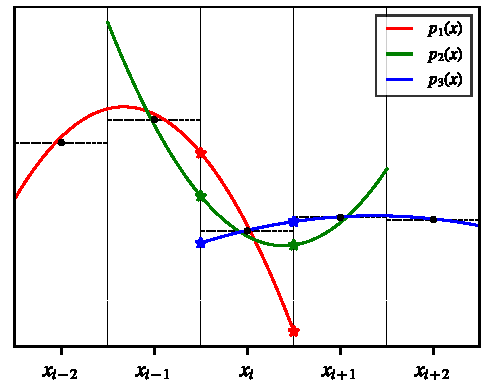
\includegraphics[width=0.85\textwidth]{fig/weno_p1p2p3}
    \caption{The reconstructed profiles in three sub-stencils of the fifth-order WENO-JS scheme.
        The black dots and horizontal dotted lines represent the volume averaged quantities.
        Note that there is a sharp discontinuity at \( x = x_{\imh} \),
        resulting three different reconstructed pointwise values at \( x = x_{i \pm \half} \)
        of each polynomial, marked as stars.
        In ENO perspective, \( p_{3} (x) \) is an appropriate choice, as \( S_{3} = \{ I_{i}, I_{i + 1}, I_{I + 2} \} \)
        does not include the discontinuous point.
    }\label{fig:weno_profiles}
\end{figure}
The core design principle of WENO is to construct nonlinear weights \( \omega_{m} \)
that adaptively select smooth stencils and converges into the linear reconstruction scheme
when all stencils are smooth. Mathematically speaking, the nonlinear weights should
be converged into the \textit{linear weights} \( \gamma_{m}, \; m = 1, 2, 3 \),
\begin{equation}\label{eq:weno_lin_weights}
    \phi (x) = \sum_{m=1}^{3} \gamma_{m} p_{m} (x),
\end{equation}
where \( \phi (x) \) is the reconstructed polynomial within the whole stencil \( S = \bigcup_{m=1}^{3} S_{m} \),
\begin{equation}\label{eq:weno_phi}
    \frac{1}{\dx} \int_{I_{k}} \phi (x) \mathop{dx} = \overline{q}_{k}, \quad
        I_{k} \in \bigcup_{m=1}^{3} S_{m}.
\end{equation}
As the \( \phi (x) \) is the quartic polynomial, it ensures fifth-order convergence rate
of the estimations for pointwise values,
\begin{equation}\label{eq:weno_phi_bigo}
    q_{i \pm \half} = \phi (x_{i \pm \half}) + \mathcal{O}(\dx^{5}).
\end{equation}

Jiang and Shu~\cite{jiang1996efficient} proposed a functional form of
the nonlinear weights by,
\begin{equation}\label{eq:weno_nonlin_weights}
    \omega_{m} = \frac{\widetilde{\omega}_{m}}{\sum_{s} \widetilde{\omega}_{s}}, \quad
        \widetilde{\omega}_{m} = \frac{\gamma_{m}}{{\left( \epsilon + \beta_{m} \right)}^{p}},
\end{equation}
where \( \epsilon \) is the small number (e.g., \( \num{1.E-36} \)) to prevent division by zero,
\( \beta_{m} \) is the smoothness indicator which measures the smoothness of the data
in the given stencil \( S_{m} \).
The parameter \( p \) is an amplification factor for the difference of scales
when a discontinuity is present on one of the candidate stencils.

The remaining step for WENO-JS is to construct the smoothness indicator,
which has large values when the stencil data is not smooth and becomes arbitrary small in a smooth stencil;
thus, it converges to the linear weight.
Jiang and Shu proposed a way to measure the smoothness of the profile based on its second derivatives.
In the fifth-order WENO-JS method, the smoothness indicators \( \beta_{m} \) are given by,
\begin{equation}\label{eq:weno_smoothness_ind}
    \beta_{m} = \sum_{n = 1}^{2} \left( \dx^{2n-1} \int_{I_{i}} {\left[ \frac{d^{n} p_{m} (x)}{dx^{n}} \right]}^{2} \mathop{dx} \right).
\end{equation}

\begin{figure}
    \centering
    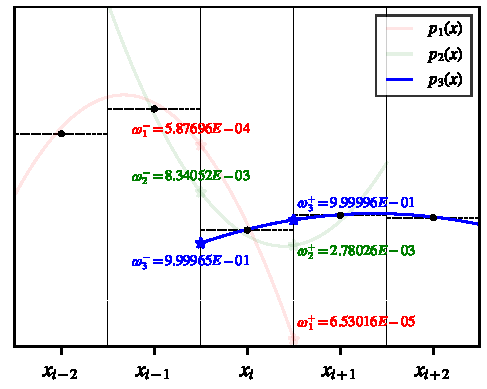
\includegraphics[width=0.85\textwidth]{fig/weno_p1p2p3_nonlinW}
    \caption{The reconstructed fifth-order WENO profiles of the same data stencil in~\cref{fig:weno_profiles},
        combined with WENO-JS nonlinear weights. (\cref{eq:weno_nonlin_weights})
        The opacity of each line measures the nonlinear weights on that sub-stencil,
        and calculated nonlinear weights are noted in the figure.
        Note that the nonlinear weights of \( S_{3} \) are dominant over other stencils, \( S_{1} \) and \( S_{2} \),
        resulting in ENO-style stencil selection.
    }\label{fig:weno_profiles_nonlinW}
\end{figure}

\cref{fig:weno_profiles_nonlinW} shows the effects of the nonlinear weights on the WENO profiles.
The nonlinear weights are calculated through~\cref{eq:weno_nonlin_weights}, with \( p = 2, \; \epsilon = \num{1.E-36} \).
As illustrated in the figure, the nonlinear weights successfully detect the sharp gradient at \( x = x_{\imh} \)
and weighting on \( p_{3} (x) \) dominantly to avoid reconstruction on the discontinuity.



\subsection{Gaussian Process Reconstruction}\label{subsec:gp}

Over decades, the high-order data reconstruction/interpolation methods
for solving hyperbolic PDEs are based on the polynomial approach.
Like the WENO method discussed in the previous section,
the idea starts by assuming a unique polynomial represents the stencil data.
The polynomial-based approaches are the most successful and popular reconstruction/interpolation methods
in the CFD community~\cite{van1979towards,colella1984piecewise,jiang1996efficient,lee2017piecewise}
because of their mathematical simplicity. 

However, the polynomial-based reconstruction/interpolation schemes have some downsides.
Firstly, since the polynomials are not able to represent the discontinuous data,
it is notoriously prone to lead numerical oscillations.
There are several ways to avoid the oscillations, like the WENO method in~\ref{subsec:weno},
but it usually brings complexity and computational expenses.
Another issue for the polynomial-based approach is that the method must be carried out
on a fixed size data stencil, which means changing in stencil size~--~thus it changes the order
of accuracy~--~requires a complete redesign of the code.

Recently, practitioners have designed \textit{non-polynomial} reconstruction/interpolation methods.
Reyes et al.~\cite{reyes2018new,reyes2019variable} proposed a novel way to use the Gaussian process (GP)
to estimate the data at any arbitrary point in high-order accuracy.
Based on the stochastic process, GP reconstruction/interpolation methods are able to predict the data
on desired points (usually at cell interfaces) without considering any polynomials;
therefore, the code is readily extended to a higher order by simply changing the size of the stencil.
In the language of GP, this process can be interpreted in the way that
a probability distribution for the unknown function values \( f(x_{*})\) (pointwise values at arbitrary points \( x_{*} \))
can be trained by the known data \( \overline{q}_{i} \) (volume-averaged quantities at cell centers),
with posterior mean and uncertainty that are compatible with the known observations.

A GP is fully defined by two functions:
\begin{itemize}
    \item a mean function \( \mu_{f} (\bx) = \mathbb{E} \left[ f(\bx) \right] \) over \( \mathbb{R}^{N} \), and
    \item a covariance kernel function, which is symmetric and positive-definite integral kernel
        \( K(\bx, \by) = \mathbb{E}\left[ \left( f(\bx) - \mu_{f} (\bx) \right) \left( f(\by) - \mu_{f} (\by) \right) \right] \)
        over \( \mathbb{R}^{N} \times \mathbb{R}^{N} \),
\end{itemize}
The function \( f \) is then said to belong to the GP with mean and covariance function,
written as \( f \sim GP(\mu_{f} (\bx), K(\bx, \by)) \).

Suppose there are \( N \) sample points for the function \( f \), namely, \( \bff = \left[ f(\bx_{1}), \dots, f(\bx_{N}) \right] \)
that are known, the likelihood \( \mathcal{L} \), the probability of \( \bff \) given the prior GP model,
of the input data \( \bff \), is given by,
\begin{equation}\label{eq:gp_likelihood}
    \mathcal{L} = P(\bff) \equiv \left( 2 \pi \right)^{- \frac{N}{2}} \det \left| \bK \right|^{-\half}
    \exp \left[ -\half \left( \bff - \bmu_{\bff} \right)^{T} \bK \left( \bff - \bmu_{\bff} \right) \right],
\end{equation}
where \( \bK = \left[ K_{ij} \right]_{i, j = 1, \dots, N} \) with \( K_{ij} = K(\bx_{i}, \bx_{j}) \).

The goal of GP is to make a probabilistic statement about the value of \( f_{*} = f (\bx_{*}) \)
of unknown function \( f \sim GP(\mu_{f}, K) \) with given function samples.
By utilizing the conditioning property of GP from the theory of Bayesian inference,
the updated posterior mean function can be obtained as,
\begin{equation}\label{eq:gp_posterior_mean_function}
    \tilde{f}_{*} \equiv \mu_{f}(\bx_{*}) + \bk_{*}^{T} \bK^{-1} \left( \bff - \bmu_{\bff} \right),
\end{equation}
where \( \bk_{*} = \left[ k_{*,i} \right]_{i = 1, \dots, N} \) with \( k_{*,i} = K(\bx_{*}, \bx_{i}) \).
The detailed derivations of \cref{eq:gp_posterior_mean_function} can be found
in the Appendix of~\cite{reyes2018new}.
It is common practice to take the zero mean everywhere, then \cref{eq:gp_posterior_mean_function} becomes
\begin{equation}\label{eq:gp_intp}
    \tilde{f}_{*} = \bk_{*}^{T} \bK^{-1} \bff,
\end{equation}
reveals GP prediction with known function samples \( \bff \), which is the \textit{pointwise} representation.

However, in the reconstruction scheme, the known function samples should be given as \textit{volume averaged} quantities,
not as pointwise values. Therefore, the GP prediction has to be modified to adapt to the data type changes.

Favorably, the volume averaging operator constitutes a linear operation (see~\cref{eq:recon_poly_linear}).
The linear operations on Gaussian random variables result in new Gaussian random variables with
linearly transformed mean and covariance; thus, the GP \textit{interpolation} scheme (\cref{eq:gp_intp})
can be transformed into the GP \textit{reconstruction} scheme
with proper linear functionals that represent volume-averaging.

Consider a measure \( dg_{k} (\bx) \) on the function \( f(\bx) \) over the cell
\( I_{k} = \prod_{d = x,y,z} I_{k}^{(d)} \) with 1D cells
\( I_{k}^{(d)} = \left[ x_{k}^{(d)} - \frac{\Delta^{(d)}}{2},\; x_{k}^{(d)} + \frac{\Delta^{(d)}}{2} \right] \),
where \( d = x,y,z \) represent the direction of the spatial dimension.
This defines the linear functionals
\begin{equation}\label{eq:gp_vol_intg}
    G_{k} \equiv \int f (\bx) \mathop{d g_{k}(\bx)},
\end{equation}
which represent the volume integral operations on \( f(\bx) \).
The measure \( dg_{k} (\bx) \) are taken to be the cell volume-average measures as,
\begin{equation}\label{eq:gp_dgk}
    dg_{k} (\bx) = \begin{cases}
        d^{3} \bx \cdot \prod\limits_{d = x,y,z} \frac{1}{\Delta^{(d)}} \quad &\text{if } \bx \in I_{k} \\
        0 &\text{otherwise},
    \end{cases}
\end{equation}
where \( \Delta^{(d)} \) is the grid spacing in the \( d \)-direction.
Then, the vector \( \bG \left[ G_{1}, \dots, G_{N} \right]^{T} \)
is normally distributed with mean \( \mathbb{E}(\bG) = \bmu_{\bG} = \left[ \mu_{G_{1}}, \dots, \mu_{G_{N}} \right]^{T} \)
and covariance matrix \( \bC = \left[ C_{kh} \right]_{k,h = 1, \dots, N} \), where
\begin{equation}\label{eq:gp_mu_G}
    \mu_{G_{k}} = \mathbb{E} [G_{k}] = \int \mathbb{E} \left[ f(\bx) \right] \mathop{d g_{k} (\bx)} = \int \mu_{f} (\bx) \mathop{d g_{k} (\bx)},
\end{equation}
and
\begin{equation}\label{eq:gp_Ckh}
    \begin{split}
        C_{kh} &= \mathbb{E} \left[ \left( G_{k} - \mu_{G_{k}} \right) \left( G_{h} - \mu_{G_{h}} \right) \right] \\
               &= \int \int \mathbb{E} \left[ \left( f(\bx) - \mu_{f} (\bx) \right) \left( f(\by) - \mu_{f} (\by) \right)\right] \mathop{d g_{k}(\bx)} \mathop{d g_{h} (\by)} \\
               &= \int \int K (\bx, \by) \mathop{d g_{k} (\bx)} \mathop{d g_{h} (\by)}.
    \end{split}
\end{equation}
Thus, the GP distribution on the function \( f \sim GP(\mu, K) \) conducts a multivariate
Gaussian distribution on \( N \)-dimensional vector \( \bG \) of linear functionals of \( f \).

In order to generalize~\cref{eq:gp_intp} for reconstruction, the remaining task is to define
the prediction vector \( \bT_{*} = \left[ \bT_{*,k} \right]_{k = 1, \dots, N} \)
at any arbitrary point of interest \( \bx_{*} \) as,
\begin{equation}\label{eq:gp_pred_vec}
    \begin{split}
        T_{*, k} &= \mathbb{E} \left[ \left( f(\bx_{*}) - \mu_{f}(\bx_{*}) \right) \left( G_{k} - \mu_{G_{k}} \right) \right] \\
                 &= \int K (\bx_{*}, \bx) \mathop{d g_{k} (\bx)}.
    \end{split}
\end{equation}
Finally, the pointwise estimation of \( f(\bx_{*}) \) at the point of \( \bx_{*} \),
reconstructed from the volume-averaged data \( \bG \) is given by,
\begin{equation}\label{eq:gp_recon}
    \tilde{f}_{*} = \bT_{*}^{T} \bC^{-1} \bG,
\end{equation}
with zero mean values. \cref{eq:gp_recon} shows the explicit form of GP reconstruction
with known volume-averaged data points, \( \bG \). The terms \( \bC \) and \( \bT \) are determined by
the choice of the covariance kernel function, \( K(\bx, \by) \), which measures the relationship between pairs of data.
In this dissertation, the ``Squared Exponential'' (SE) kernel used for GP reconstruction.
\begin{equation}\label{eq:gp_se_kernel}
    K_{\text{SE}} (\bx, \by) = \Sigma^{2} \exp \left[ -\frac{\left( \bx - \by \right)^{2}}{2 \ell^{2}} \right].
\end{equation}
The SE kernel has two hyperparameters \( \Sigma \) and \( \ell \),
but the hyperparameter \( \Sigma \) has no effect on the posterior mean function,
so this dissertation set \( \Sigma = 1 \) for simplicity.
On the other hand, the hyperparameter \( \ell \) expresses the correlation length scale of the model,
so it should be chosen meticulously corresponding to the physical length scale of the grid configuration.

For 1D reconstructions, \( T_{*, k} \) and \( C_{kh} \) for SE kernel becomes,
\begin{equation}\label{eq:gp_se_T}
    T_{*,k} = \sqrt{\frac{\pi}{2}}\frac{\ell}{\Delta} \left \{
        \erf{\frac{\Delta_{k*}+1/2}{\sqrt{2}\ell/\Delta}}
        - \erf{\frac{\Delta_{k*}-1/2}{\sqrt{2}\ell/\Delta}}
     \right \},
\end{equation}
and
\begin{equation}\label{eq:gp_se_C}
    \begin{split}
        C_{kh} = \sqrt{\pi} & \left( \frac{\ell}{\Delta} \right)^{2}
        \left \{
            \left( \frac{\Delta_{kh} + 1}{\sqrt{2} \ell / \Delta} \erf{\frac{\Delta_{kh} + 1}{\sqrt{2} \ell / \Delta}} +
                \frac{\Delta_{kh} - 1}{\sqrt{2} \ell / \Delta} \erf{\frac{\Delta_{kh} - 1}{\sqrt{2} \ell / \Delta}}
            \right) \right. \\
            &+ \frac{1}{\sqrt{\pi}} \left(
                \exp \left[ - \frac{\left( \Delta_{kh} + 1 \right)^{2}}{2 \left( \ell / \Delta \right)^{2}} \right]
                + \exp \left[ - \frac{\left( \Delta_{kh} -1 \right)^{2}}{2 \left( \ell / \Delta \right)^{2}} \right]
            \right) \\
            &\left.
            -2 \left(
                \frac{\Delta_{kh}}{\sqrt{2} \ell / \Delta} \erf{\frac{\Delta_{kh}}{\sqrt{2} \ell / \Delta}}
                + \frac{1}{\sqrt{\pi}} \exp \left[ -\frac{\Delta_{kh}^{2}}{2 \left( \ell / \Delta \right)^{2}} \right] 
            \right)
        \right \},
    \end{split}
\end{equation}
where \( \Delta_{kh} = (x_{k} - x_{h})/\Delta \) and \( \Delta \) is the grid spacing along the 1D direction.
Note that the analytic derivations of \( T_{*, k} \) and \( C_{kh} \) above
only depend on the grid spacing and the length between the prediction point \( \bx_{*} \)
and the locations of known training data. With uniform grid configuration,
those values are established at the initial step.
Since the prediction points are the cell interfaces \( x_{i \pm \half} \)
for the conventional FDM constructions, one can save,
\begin{equation}\label{eq:gp_zvec}
    \bz_{i \pm \half} \coloneqq \bT^{T}_{i \pm \half} \bC^{-1},
\end{equation}
as the weighting factor for the reconstruction can be expressed as,
\begin{equation}\label{eq:gp_recon_with_zvec}
    q_{i \pm \half} = \bz^{T}_{i \pm \half} \bG,
\end{equation}
for computational efficiency.

\begin{figure}
    \centering
    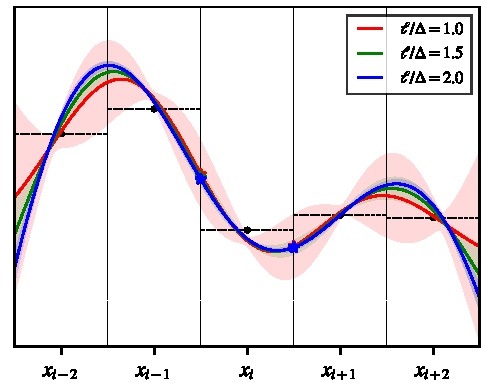
\includegraphics[width=0.85\textwidth]{fig/gp_linear_recon}
    \caption{GP reconstructed profiles with the same data as~\cref{fig:weno_profiles,fig:weno_profiles_nonlinW}
        with different hyperparameters \( \ell = 1.0, 1.5, 3.0 \).
        Note that all the reconstructed profiles produce a new local minimum near \( x = x_{\iph} \),
        which violates the monotonic-preserving condition and leads to numerical oscillations.
        The shaded areas represent 95\% confidence regions from the posterior variance.
    }\label{fig:gp_linear_recon}
\end{figure}

However, the GP reconstruction also needs special handling for the discontinuous profiles,
like the nonlinear weightings in the WENO method in~\cref{subsec:weno}.
\cref{fig:gp_linear_recon} shows the GP reconstructions with the same data as~\cref{fig:weno_profiles,fig:weno_profiles_nonlinW},
with \( \ell = 1, 1.5, 3 \). The initial profile has a strong gradient at \( x = x_{\imh} \);
hence, the GP reconstructed profiles have undershot values at \( x = x_{\iph} \).

Reyes et al.~\cite{reyes2019variable} proposed a WENO-\textit{like} approach to
the GP reconstruction/interpolations by considering the GP marginal likelihood of the local stencil data
for measuring the smoothness of the stencil,
and use them to construct nonlinear weights as like in the standard WENO method.

For five points, fifth-order GP reconstruction, suppose three sub-stencils as like fifth-order WENO method. (\cref{eq:weno_substencils})
Then there are three reconstructed pointwise values for each of the candidate stencils \( S_{m} \),
\begin{equation}\label{eq:gp_weno_candidates}
    q_{i \pm \half, m} = \bz_{i \pm \half, m}^{T} \bG_{m}.
\end{equation}
The final reconstructed value is taken as the combinations of three candidate GP approximations with nonlinear weights,
\begin{equation}\label{eq:gp_weno_comb}
    q_{i \pm \half} = \sum_{m = 1}^{3} \omega_{m} q_{i \pm \half, m}.
\end{equation}

As in the conventional WENO method, the nonlinear weights \( \omega_{m} \)
must be reduced to the optimal (linear) weights \( \gamma_{m} \) in a smooth region,
so the weighted combination~\cref{eq:gp_weno_comb} converges to the GP approximation
over the whole stencil \( S = \bigcup_{m} S_{m} \). The optimal weights \( \gamma_{m} \) must satisfy,
\begin{equation}\label{eq:gp_weno_linW}
    \bz_{i \pm \half}^{T} \bG = q_{i \pm \half} = \sum_{m=1}^{3} \gamma_{m} q_{i \pm \half, m} = \sum_{m=1}^{3} \gamma_{m} \bz_{i \pm \half, m}^{T} \bG_{m},
\end{equation}
or explicitly,
\begin{equation}\label{eq:gp_weno_overdetermined}
    \gamma_{1}
    \left[
        \begin{array}{c}
            \mathrm{z}_{1,1}^{\pm} \\
            \mathrm{z}_{2,1}^{\pm} \\
            \mathrm{z}_{3,1}^{\pm} \\
            0 \\
            0 \\
        \end{array}
    \right]
    \hspace{-30.0\arrayrulewidth}
    \begin{array}[c]{@{}l@{\,}l}
       \left.
       \begin{array}{c}
           \vphantom{\vdots}\\
           \vphantom{0}
       \end{array}
       \right\}
       &
       {\bz_{i \pm \half, 1}} \\ \\ \\
    \end{array}
    \hspace{-20.0\arrayrulewidth}
+
    \gamma_{2}
    \left[
        \begin{array}{c}
            0 \\
            \mathrm{z}_{1,2}^{\pm} \\
            \mathrm{z}_{2,2}^{\pm} \\
            \mathrm{z}_{3,2}^{\pm} \\
            0 \\
        \end{array}
    \right]
    \hspace{-30.0\arrayrulewidth}
    \begin{array}[c]{@{}l@{\,}l}
       \left.
       \begin{array}{c}
           \vphantom{\vdots}\\
           \vphantom{0}
       \end{array}
       \right\}
       &
       {\bz_{i \pm \half, 2}} \\
    \end{array}
    \hspace{-20.0\arrayrulewidth}
+
    \gamma_{3}
    \left[
        \begin{array}{c}
            0 \\
            0 \\
            \mathrm{z}_{1,3}^{\pm} \\
            \mathrm{z}_{2,3}^{\pm} \\
            \mathrm{z}_{3,3}^{\pm} \\
        \end{array}
    \right]
    \hspace{-30.0\arrayrulewidth}
    \begin{array}[c]{@{}l@{\,}l} \\ \\
       \left.
       \begin{array}{c}
           \vphantom{\vdots}\\
           \vphantom{0}
       \end{array}
       \right\}
       &
       {\bz_{i \pm \half, 3}}
    \end{array}
    \hspace{-20.0\arrayrulewidth}
=
    \left[
        \begin{array}{c}
            \mathrm{z}_{1}^{\pm} \\
            \mathrm{z}_{2}^{\pm} \\
            \mathrm{z}_{3}^{\pm} \\
            \mathrm{z}_{4}^{\pm} \\
            \mathrm{z}_{5}^{\pm} \\
        \end{array}
    \right]
    \hspace{-30.0\arrayrulewidth}
    \begin{array}[c]{@{}l@{\,}l}
       \left.
       \begin{array}{c}
           \vphantom{0} \\
           \vphantom{\vdots} \\
           \vphantom{\vdots} \\
           \vphantom{0}
           \end{array}
       \right\}
       &
       \bz_{i \pm \half} \\
    \end{array}.
\end{equation}
The \cref{eq:gp_weno_overdetermined} can be rewritten in the matrix form
of overdetermined system as,
\begin{equation}\label{eq:gp_weno_overdetermined_matrix}
    \left[ 
        \begin{array}{ccc}
            {\mathrm{z}_{1,1}^{\pm}}  & 0                       & 0 \\
            {\mathrm{z}_{2,1}^{\pm}}  & \mathrm{z}_{1,2}^{\pm}  & 0 \\
            {\mathrm{z}_{3,1}^{\pm}}  & \mathrm{z}_{2,2}^{\pm}  & \mathrm{z}_{1,3}^{\pm} \\
            0                         & \mathrm{z}_{3,2}^{\pm}  & \mathrm{z}_{2,3}^{\pm} \\
            0                         & 0                       & \mathrm{z}_{3,3}^{\pm} \\
        \end{array}
    \right]
%
\left[
    \begin{array}{c}
        \gamma_1\\
        \gamma_2\\
        \gamma_3\\
    \end{array}
\right]
%
=
%
\left[
    \begin{array}{c}
        {\mathrm{z}_{1}^{\pm}} \\
        {\mathrm{z}_{2}^{\pm}} \\
        {\mathrm{z}_{3}^{\pm}} \\
        {\mathrm{z}_{4}^{\pm}} \\
        {\mathrm{z}_{5}^{\pm}} \\
    \end{array}
\right].
\end{equation}
Thus, the optimal weights \( \gamma_{m}, m = 1, 2, 3 \) are obtained by solving the overdetermined system,
\cref{eq:gp_weno_overdetermined_matrix}. It should be noted that the optimal weights are
entirely determined by the choice of kernel function and the stencil size,
so they are computed and stored before the simulation begins.

For constructing WENO nonlinear weights~\cref{eq:weno_nonlin_weights},
the only remaining task is to determine the smoothness indicator, \( \beta_{m} \),
which measures the degree of smoothness of a given stencil of data.
Unlike the conventional WENO method, which measures the smoothness of the data
by calculating \( L_{2} \) norms of all the derivatives of the reconstructed polynomials,
the GP reconstruction method should take a different approach to specify the smoothness indicator
because there is no polynomial defined in GP\@.
One successful practice is to use the marginal likelihood of the data.
The likelihood function is well-furnished to gauge the deviations from smoothness
given a sufficiently smooth covariance kernel function, SE kernel, for example.
Thus, the GP predictions have smaller likelihoods to non-smooth function by its design.

Suppose the negative log of the GP marginal likelihood as
\begin{equation}\label{eq:gp_log_marginal_likelihood}
    -\log \mathcal{L} = \frac{N}{2} \log \left[ 2 \pi \right] + \half \log \left| \det \bK_{m} \right|
        + \half \left( \bff_{m} - \bmu_{\bff} \right)^{T} \bK_{m}^{-1} \left( \bff_{m} - \bmu_{\bff} \right),
\end{equation}
then the three terms on the right-hand side of~\cref{eq:gp_log_marginal_likelihood} are revealed as
a normalization, a complexity penalty, and a data fit term, respectively.
The normalization term and the complexity penalty have no effects on defining smoothness indicators
in a uniform grid configuration; only the data fit term along with the choice of zero mean is used
for constructing smoothness indicators in GP,
\begin{equation}\label{eq:gp_smoothness_ind}
    \beta_{m} = \bff_{m}^{T} \left( \bK^{-1}_{m} \right) \bff_{m}.
\end{equation}
To handle discontinuity, a second hyperparameter, \( \sigma \), should be used in~\cref{eq:gp_smoothness_ind},
to discriminate discontinuities from smooth regions. \( \sigma \) should be on the order of the grid spacing.

Like GP reconstruction weights~\cref{eq:gp_recon_with_zvec}, the calculations of
GP smoothness indicators \( \beta_{m} \) can be expressed in a more computationally efficient form.
Considering the eigensystem \( \bK_{m}^{-1} = \sum_{i} \mathbf{v}_{i}^{m} \left( \mathbf{v}_{i}^{m} \right)^{T}/\lambda_{i}^{m} \),
\begin{equation}\label{eq:gp_smoothness_ind_with_eig}
    \beta_{m} = \sum_{i=1}^{3} \bff_{m}^{T} \left( \frac{\mathbf{v}_{i}^{m} \left( \mathbf{v}_{i}^{m} \right)^{T}}{\lambda_{i}} \right) \bff_{m},
\end{equation}
in the five-point, three-stencil GP-WENO method\@.
Again, the observed (training) data is in the volume-averaged form;
thus, the data-type conversion should be examined:
\begin{equation}\label{}
    \bff_{m} = \mathbf{Z}_{m}^{T} \bG_{m},
\end{equation}
where each column vector of \( \mathbf{Z}_{m} \) is given by the GP reconstructing weight, \( \bz \), (see~\cref{eq:gp_zvec})
for each elements of \( \bff_{m} \).

Lastly, the calculation of the smoothness indicator beta can be expressed in the compact form as,
\begin{equation}\label{eq:gp_weno_smooth_ind}
    \begin{split}
        \beta_{m} &= \sum_{i=1}^{3} \left( \frac{ \left( \mathbf{v}_{i}^{m} \right)^{T} \mathbf{Z}_{m}^{T} \bG_{m} }{\sqrt{\lambda_{i}^{m}}} \right)^{2} \\
                  &= \sum_{i=1}^{3} \left( \bP_{i}^{m} \bG_{m} \right)^{2},
    \end{split}
\end{equation}
where \( \bP_{i}^{m} \coloneqq \frac{ \left(\mathbf{v}_{i}^{m}\right)^{T} \mathbf{Z}_{m}^{T}}{\sqrt{\lambda_{i}^{m}}} \),
which can be established before the simulation start, in uniform grid configuration.

Now, the nonlinear weights for GP-WENO reconstruction are fully determined
with~\cref{eq:weno_nonlin_weights}.
In the stepwise representation, the GP-WENO reconstruction scheme for FDM formulation
in the unifrom grid can be summarized as below:
\begin{enumerate}
    \item Before the simulation starts, calculate the following values and store them for later reconstructions:
        \begin{enumerate}
            \item Reconstruction weights, \( \bz_{m} \) (\cref{eq:gp_weno_candidates}) for each candidate stencil, \( m \).
            \item Linear weights, \( \gamma_{m} \), by the solving overdetermined system, \cref{eq:gp_weno_overdetermined_matrix},
                using the least square method.
            \item \( \bP_{i}^{m} \) (\cref{eq:gp_weno_smooth_ind}) for calculating smoothness indicator \( \beta_{m} \) in later.
        \end{enumerate}
    \item During the simulation, at each reconstruction step of cell \( I_{i} \):
        \begin{enumerate}
            \item Calculate nonlinear weights, \( \omega_{m} \), following the conventional WENO method. (\cref{eq:weno_nonlin_weights})
            \item Compute \( m \)-number of reconstructed candidate data, \( q_{i \pm \half, m} \). (\cref{eq:gp_weno_candidates})
            \item Taking weighted combinations of \( q_{i \pm \half, m} \), with nonlinear weights, \( \omega_{m} \),
                and finalize the reconstruction step at \( x_{i} = x_{i \pm \half} \). (\cref{eq:gp_weno_comb})
        \end{enumerate}
\end{enumerate}

\begin{figure}
    \centering
    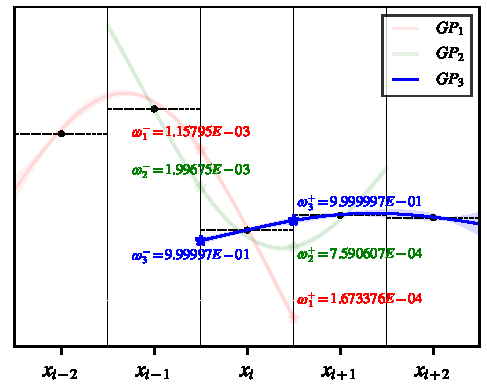
\includegraphics[width=0.85\textwidth]{fig/gp_weno_nonlinW}
    \caption{GP-WENO Reconstructed profiles with nonlinear weights with the same data as~\cref{fig:gp_linear_recon}.
        Hyperparameters \( \ell = 2\Delta \) and \( \sigma = 2\Delta \) are used. 95\% confidence regions
        are shaded with the correspoinding colors, and the opacity of each prediction measures the nonlinear weights
        on that sub-stencil.
    }\label{fig:gp_weno_nonlinW}
\end{figure}




\section{High-Order Time Integration Schemes}\label{sec:time_integration}

A high-order temporal discretization scheme ought to be considered alongside
the high-order spatial data interpolation/reconstruction to acquire
highly accurate numerical solutions in FDM formulation.
The numerical errors arise from both spatial and temporal discretizations
since the solution of the conservative PDEs lies on the spatio-temporal plane.
The overall order of solution accuracy will be determined by the highest order term
of the truncation errors both from the spatial and temporal discretization, i.e.,
\( \mathcal{O}(\Delta s^{p}, \Delta t^{q}) \).
For example, if the leading error term from the temporal discretization
is significantly larger than the leading error term from the spatial discretizations,
\( \mathcal{O}(\dt^{q}) > \mathcal{O}(\Delta s^{p}) \),
then the solution accuracy will be degraded by order of temporal accuracy, \( q \),
no matter the order of spatial accuracy is used.
Therefore, a high-order FDM scheme requires a meticulously designed
temporal discretization method that ensures the solution’s accuracy and stability.

\subsection{Strong Stability Preserving Runge-Kutta Methods}\label{subsec:ssprk}

The Runge-Kutta (RK) method is the most popular way to integrate
the semi-discretized form of FDM (\cref{eq:fdm_discrete}) over the time axis.
The key idea is to treat the~\cref{eq:fdm_discrete} as an ordinary differential equation (ODE)
at each lattice point on the computational mesh as,
\begin{equation}\label{eq:fdm_mol}
    \pd{\bU_{i}}{t} = \mathcal{L}_{i} (\bU),
\end{equation}
where the right-hand side operator \( \mathcal{L}_{i} \) is given by the spatial discretization method at cell \( I_{i} \).
The RK approach can be viewed as a strategy to integrate PDEs by solving several ODE problems at each discretized time domain.
In general, \( m \)-stage RK method which integrate~\cref{eq:fdm_mol}
from \( t = t^{n} \) to \( t = t^{n} + \dt = t^{n + 1} \) is given by,
\begin{equation}\label{eq:general_rk}
    \begin{split}
        \bU^{(0)} &= \bU^{n}, \\
        \bU^{(l)} &= \sum_{k=0}^{l -1} \left( \alpha_{l, k} \bU^{(k)} + \dt \beta_{l,k} \mathcal{L} (\bU^{(k)}) \right), \quad \alpha_{l,k} \geq 0, \quad l = 1, \dots, m \\
        \bU^{n + 1} &= \bU^{(m)},
    \end{split}
\end{equation}
where the spatial discretization index, \( i \), is omitted for simplicity.
Therefore, the coefficients \( \alpha_{l,k} \) and \( \beta_{l,k} \) fully determine
the numerical accuracy and stability of the RK scheme.

Like the spatial discretization method, it is crucial to consider the TVD property of the temporal discretization scheme.
Gottlieb and her collaborators~\cite{gottlieb1998total,gottlieb2001strong,gottlieb2011strong}
developed the so-called strong stability preserving Runge-Kutta (SSP-RK) method,
which ensures TVD property by sequentially applying convex combinations of the
first-order forward Euler method as a building-block at each sub-stage.
In this way, the desired TVD property is achieved if each of the sub-stage is TVD\@.

SSP-RK method uses that the forward Euler method for building each sub-stages.
Since the forward Euler method is strongly stable under the Courant–Friedrichs–Lewy (CFL) condition;
thus, if all sub-stages of the RK method can be described as a form of the forward Euler method,
then the TVD property is fulfilled by virtue of the forward Euler method.
It is easy to see in~\cref{eq:general_rk} that the sub-stages of the RK method, \( \bU^{(l)} \)
can be described as the forward Euler method if all the \( \beta_{l, k} \) are nonnegative \( \beta_{l, k} \geq 0 \)
by replacing \( \dt \) by \( \frac{\beta_{l, k}}{\alpha_{l, k}} \dt \).
For example, in~\cite{gottlieb1998total}, Gottlieb found the optimal third-order
SSP-RK method given by,
\begin{equation}\label{eq:ssp_rk3}
    \begin{split}
        \bU^{(1)} &= \bU^{n} + \dt \mathcal{L}(\bU^{n}), \\
        \bU^{(2)} &= \frac{3}{4} \bU^{n} + \frac{1}{4} \bU^{(1)} + \frac{1}{4} \dt \mathcal{L}(\bU^{(1)}), \\
        \bU^{n + 1} &= \frac{1}{3} \bU^{n} + \frac{2}{3} \bU^{(2)} + \frac{2}{3} \dt \mathcal{L}(\bU^{(2)}),
    \end{split}
\end{equation}
which requires three sub-stages for integrating from \( t = t^{n} \) to \( t = t^{n + 1} \).

The above third-order, three-stages SSP-RK method~\cref{eq:ssp_rk3} is by far
the most famous high-order time integrator used in most high-order method researches in the CFD community.
In practice, spatial accuracy is often considered to carry more weight than temporal accuracy
in designing higher accurate spatial models~\cite{balsara2000monotonicity,mignone2010high},
so combining the high-order spatial method (generally, fifth-order or higher)
with a relatively low-order temporal scheme (third-order SSP-RK) could be justifiable.
However, as it is shown in~\cite{lee2021recursive}, the order of convergence rate of the solution
can be degraded by the order of temporal method (e.g., third-order) in high-resolution computational grids,
so using a higher than third-order temporal scheme is required for maintaining desired spatial accuracy in a high-resolution grid.

In contrast to the third-order SSP-RK3 method, devising a fourth-order SSP-RK4
is more involved to meet the favorable SSP property, which is ensured by positive coefficients.
Several theoretical studies have shown that a fourth-order SSP-RK4
cannot be formulated with just four sub-stages and positive coefficients~\cite{gottlieb1998total},
meaning that the classical four-stage, fourth-order RK is not SSP\@.
For example, by far the most optimal fourth-order, fourth-stage SSP-RK method is:
\begin{equation}\label{eq:ssp_rk44_negatives}
    \begin{split}
        \bU^{(1)} &= \bU^{n} + \half \dt \mathcal{L}(\bU^{n}), \\
        \bU^{(2)} &= \frac{649}{1600} \bU^{(0)} - \frac{10890423}{25193600} \dt \tilde{\mathcal{L}} (\bU^{n}) + \frac{951}{1600} \bU^{(1)} + \frac{5000}{7873} \dt \mathcal{L}(\bU^{(1)}), \\
        \bU^{(3)} &= \frac{53989}{2500000} \bU^{n} - \frac{102261}{5000000} \dt \tilde{\mathcal{L}} (\bU^{n}) + \frac{4806213}{20000000} \bU^{(1)} \\
            &\quad - \frac{5121}{20000} \dt \tilde{\mathcal{L}}(\bU^{(1)}) + \frac{23619}{32000} \bU^{(2)} + \frac{7873}{10000} \dt \mathcal{L}(\bU^{(2)}), \\
        \bU^{(4)} &= \frac{1}{5} \bU^{n} + \frac{1}{10} \dt \mathcal{L}(\bU^{n}) + \frac{6127}{30000} \bU^{(1)} + \frac{1}{6} \dt \mathcal{L}(\bU^{(1)}) + \frac{7873}{30000} \bU^{(2)} \\
            &\quad + \frac{1}{3} \bU^{(3)} + \frac{1}{6} \dt \mathcal{L}(\bU^{(3)}).
    \end{split}
\end{equation}
Note that the above four-stage, fourth-order SSP-RK method uses the adjoint spatial operator, \( \tilde{\mathcal{L}} \),
to bear the negative coefficients, e.g., \( -\frac{10890423}{25193600} \) and \( -\frac{102261}{5000000} \).
Numerically speaking, the only difference between \( \mathcal{L} \) and \( \tilde{\mathcal{L}} \)
is the direction of the upwind limiting. Although the computational cost of calculating \( \mathcal{L}(\bU) \) and
\( \tilde{\mathcal{L}}(\bU) \) are identical, but it demands separated codes, and leads implementation complexity.

Spiteri and Ruuth~\cite{spiteri2002new} proposed a five-stage, fourth-order SSP-RK4 method that does not require to use adjoint operator:
\begin{equation}\label{eq:ssp_rk4}
    \begin{split}
        \bU^{(1)} &= \bU^{n} + 0.391752226571890 \dt \mathcal{L}(\bU^{n}), \\
        \bU^{(2)} &= 0.444370493651235 \bU^{n} + 0.555629506348765 \bU^{(1)} + 0.368410593050371 \dt \mathcal{L} (\bU^{(1)}), \\
        \bU^{(3)} &= 0.620101851488403 \bU^{n} + 0.379898148511597 \bU^{(2)} + 0.251891774271694 \dt \mathcal{L} (\bU^{(2)}), \\
        \bU^{(4)} &= 0.178079954393132 \bU^{n} + 0.821920045606868 \bU^{(3)} + 0.544974750228521 \dt \mathcal{L} (\bU^{(3)}), \\
        \bU^{n + 1} &= 0.517231671970585 \bU^{(2)} + 0.096059710526147 \bU^{(3)} + 0.063692468666290 \dt \mathcal{L} (\bU^{(3)}) \\
                    &\quad + 0.386708617503268 \bU^{(4)} + 0.226007483236906 \dt \mathcal{L} (\bU^{(4)}).
    \end{split}
\end{equation}
In this dissertation, the fourth-order SSP-RK4 method refers the Spiteri and Ruuth method,~\cref{eq:ssp_rk4}.

In many studies about high-order CFD solvers~\cite{gottlieb1998total,gottlieb2001strong,gottlieb2011strong,mignone2010high,del2003efficient,del2007echo,reyes2018new,reyes2019variable},
the SSP-RK schemes have proven high fidelity and portability, guaranteeing high-order accuracy
and numerical stability with TVD property.
However, the very nature of the SSP-RK method~-- being a multi-stage approach --~increases
computational costs in CFD simulations.
In SSP-RK methods, the data reconstruction/interpolation (i.e., \( \mathcal{L}(\cdot) \)) and the boundary condition
should be applied in each sub-stage, which increases the computational resources
and the footprint of data communications in the parallel computational architecture.
It makes the simulations using the adaptive mesh refinement (AMR) method less attractive,
which progressively refines the grid resolutions
and increases data communications around the simulations’ interesting features.


\subsection{Lax–Wendroff Type Methods}\label{subsec:laxwendroff}

The Lax-Wendroff method~\cite{lax1959systems} rely on the Taylor expansion in time
to achieve high-order in time accuracy:
\begin{equation}\label{eq:lw_time_taylor}
    \bU^{n + 1} = \bU^{n} + \dt \left. \pd{\bU}{t} \right|^{n} + \frac{\dt^{2}}{2!} \left.\pdd{\bU}{t}\right|^{n} + \mathcal{O}(\dt^{3}).
\end{equation}
The temporal derivatives can be transformed into spatial derivatives
by applying the Lax-Wendroff or Cauchy-Kowalewski procedure (LW/CK hereafter).
In one-dimensional conservative PDEs, for example,
\begin{equation}\label{eq:lw_1d_ck_procedure}
    \begin{split}
        \pd{\bU}{t} &= -\pd{\bF}{x}, \\
        \pdd{\bU}{t} &= \pd{}{t} \left( -\pd{\bF}{x}\right) \\
                     &= -\pd{}{x} \left( \pd{\bF}{\bU} \cdot \pd{\bU}{t} \right) \\
                     &= \pd{}{x} \left( \pd{\bF}{\bU} \cdot \pd{\bF}{x} \right),
    \end{split}
\end{equation}
where \( \pd{\bF}{\bU} \) is a flux Jacobian matrix.
In the original Lax-Wendroff method~\cite{lax1959systems} used an approximation of \( \pd{}{x} \left( \pd{\bF}{\bU} \cdot \pd{\bF}{x} \right) \approx
\frac{1}{\dx}\left( \left.\pd{\bF}{\bU} \right|_{\iph} \cdot \pd{\bF}{x} - \left.\pd{\bF}{\bU} \right|_{\imh} \cdot \pd{\bF}{x} \right) \),
but it is possible to get an explicit form as,
\begin{equation}\label{}
    \pdd{\bU}{t} = \pd{}{x} \left( \pd{\bF}{\bU} \cdot \pd{\bF}{x} \right) = \pdd{\bF}{\bU} \cdot \pd{\bF}{x} + \pd{\bF}{\bU} \cdot \pdd{\bF}{x},
\end{equation}
with flux Hessian tensor, \( \pdd{\bF}{\bU} \).

The primary advantage of the Lax-Wendroff method is that
it can achieve a high order in time accuracy within a single step of the calculation.
The idea to construct the time-Taylor series by harnessing the tight coupling of temporal
and spatial derivatives through LW/CK procedures inspires many practitioners
to develop single-step, high-order methods based on the Lax-Wendroff method.

In 2001, Toro et al.~\cite{toro2001towards} extended this idea
by combining it with the generalized Riemann problems (GRPs)
and introduced the Arbitrary high order derivative Riemann problem (ADER) method.
Toro and his collaborators constructed Riemann problems for each spatial derivative at cell interface, \( x_{\iph} \):
\begin{equation}\label{eq:toro_ader_dudx}
    \begin{split}
        &\pd{\bU^{(k)}_{x}}{t} + \left. \pd{\bF}{\bU} \right|_{\iph} \pd{\bU^{(k)}_{x}}{x} = 0, \quad \text{where } \left. \pd{\bF}{\bU} \right|_{\iph} = \pd{\bF}{\bU}(\bU_{\iph}, 0^{+}), \\
        &\bU^{(k)}_{x} (x, 0) =
        \begin{cases}
            \frac{\partial^{k}}{\partial x^{k}} \bU_{\iph, L}, \quad x < x_{\iph}, \\
            \frac{\partial^{k}}{\partial x^{k}} \bU_{\iph, R}, \quad x > x_{\iph},
        \end{cases}
    \end{split}
\end{equation}
where \( \bU^{(k)}_{x} = \frac{\partial^{k} \bU}{\partial x^{k}} \), and
\( \bU_{\iph, LR} \) represent left and right Riemann states at cell interface, \( x_{\iph} \).
Reconstructed profiles can find the Riemann states of the spatial derivatives.
The resulting solutions of the above Riemann problems
are then applied for LW/CK procedures to get the temporal derivatives, \( \left. \frac{\partial^{k} \bU}{\partial t^{k}} \right|_{\iph} \),
and they are used to construct the time-Taylor series of the conservative variables at cell interfaces:
\begin{equation}\label{eq:toro_ader}
    \bU (x_{\iph}, \tau) = \bU(x_{\iph}, 0^{+}) + \sum_{k = 1}^{r -1} \left[ \frac{\partial^{k}}{\partial t^{k}} \bU (x, t) (x_{\iph}, 0^{+}) \right] \frac{\tau^{k}}{k!}.
\end{equation}
% Toro and his collaborators applied LW/CK procedures
% to get the coefficients of the power series expansion of the conservative variables
% and solved GRPs for each high-order term.
% For instance, Toro considered a time-Taylor series of conservative variables
% at cell interface, \( \bU_{\iph} \), in arbitrary order as,

ADER methods were further developed in~\cite{toro2001towards,titarev2002ader,titarev2005ader},
and it has grown its popularity over decades,
leading to various further modifications.
ADER-DG~\cite{fambri2017space,zanotti2016efficient} and
ADER-CG~\cite{balsara2009efficient,balsara2013efficient,balsara2017higher}
in the context of discontinuous and continuous Galerkin schemes;
other efforts of employing
an implicit GRP solver
to solve  scalar equations 
with stiff source terms~\cite{montecinos2012solver},
its extensions to second-order schemes for 
nonlinear systems~\cite{montecinos2014reformulations}
and to general hyperbolic systems~\cite{toro2015implicit}.
The use of an implicit time Taylor series expansion for GRP
was further simplified
in the study by Montecinos and Balsara~\cite{montecinos2020simplified}.
Along the line of simplifying the standard ADER approach,
the Differential Transform Method (DTM)~\cite{chen1996application}
was also adopted to alleviate
the cost of the ADER scheme, coined as ADER-DT (or ADER-Taylor)
in~\cite{norman2012multi,norman2013algorithmic,norman2014weno}.

In general, Lax-Wendroff type methods are able to update the solution
in single-step with high-order temporal accuracy.
The fundamental advantage of being a single-stage method is the enhanced performance.
This becomes hugely attractive in massively parallel computing, minimizing the computational frequency
of data transfers between processors each time step, which would need to be repeated for each intermediate RK stage.
On the other hand, the dependence of the strong coupling on analytic derivatives
of the governing PDEs makes the LW/CK approach less flexible and less broadly applicable to all systems of PDEs.


\chapter{System-Free Picard Integral Formulation}\label{chap:sfpif}

Unlike the broad usage of SSP-RK in various discrete PDE solvers,
the developments of ADER mentioned above have been exclusively applied to FV and DG methods, but FD methods.
This is mainly because the fundamental principle of obtaining high-order accuracy
in the original ADER scheme relies on solving generalized (or high-order) Riemann problems,
which are the characteristic building blocks of FV and DG methods.

Recently, Christlieb et al.\ introduced a new high-order temporal scheme for FDM,
the so-called Picard integral formulation (PIF) method.~\cite{christlieb2015picard,seal2016explicit}
The PIF discretization is based on the constructions of high-order approximation
to the time-averaged fluxes over \( \left[ t^{n}, t^{n + 1} \right] \),
allowing high-order temporal accuracy in a single-step update.
Firstly introduced in~\cite{christlieb2015picard},
the PIF method demonstrated third-order temporally accurate numerical fluxes
by computing the coefficients of the time-Taylor expansion of the averaged fluxes
via LW/CK procedure which converts the high-order temporal derivatives terms into the spatial derivatives.

However, like many Lax-Wendroff type methods, the PIF method requires
finding analytic derivations for flux Jacobians and Hessians.
Although the Jacobian and the Hessian calculations can be easily obtained
with the aid of symbolic manipulators such as \texttt{SymPy}, \texttt{Mathematica}, or \texttt{Maple},
it still demands complicated coding/debugging efforts and ample memory consumption.
Furthermore, as the Jacobian/Hessian calculations highly depend on the
type of the governing system under consideration,
it is required to re-derive the Jacobian/Hessian terms analytically every time
we need to solve a new system, e.g., shallow water equations or magnetohydrodynamics (MHD) equations, to name a few.
In addition, the calculation complexities of the Jacobian-like terms are drastically increasing
with the number of spatial dimensions and the order of accuracy.



\section{Picard Integral Formulation}\label{sec:pif}
Applying the Picard integral formulation (PIF), the governing equations~\cref{eq:gov} can be discretized
by taking a time average within a single time step \( \dt \) over an interval \( \left[ t^{n}, t^{n + 1} \right] \),
\begin{equation}\label{eq:pif_time_avg}
    \bU^{n + 1} = \bU^{n} - \dt \left( \partial_{x} \bF^{avg} + \partial_{y} \bG^{avg} + \partial_{z} \bH^{avg} \right),
\end{equation}
where \( \bF^{avg}, \bG^{avg}, \) and \( \bH^{avg} \) are the time-averaged fluxes in each direction,
\begin{equation}\label{eq:pif_avg_flux}
    \begin{split}
        \bF^{avg} (\bx) = \frac{1}{\dt} \int_{t^{n}}^{t^{n + 1}} \bF (\bU(\bx, t)) \mathop{dt}, \\
        \bG^{avg} (\bx) = \frac{1}{\dt} \int_{t^{n}}^{t^{n + 1}} \bG (\bU(\bx, t)) \mathop{dt}, \\
        \bH^{avg} (\bx) = \frac{1}{\dt} \int_{t^{n}}^{t^{n + 1}} \bH (\bU(\bx, t)) \mathop{dt}, \\
    \end{split}
\end{equation}
for \( \bx = (x, y, z) \in \mathbb{R}^{3} \).

The goal is to express the spatial derivatives of the time-averaged fluxes in~\cref{eq:pif_time_avg}
using highly approximated numerical fluxes \( \hat{\bff}, \hat{\bg}, \) and \( \hat{\bh} \)
at cell interfaces:
\begin{equation}\label{eq:pif_num_flux}
    \begin{split}
        \left. \partial_{x} \bF^{avg} \right|_{\bx = \bx_{ijk}} &=
            \frac{1}{\dx} \left( \hat{\bff}_{\iph, j, k} - \hat{\bff}_{\imh, j, k} \right) + \mathcal{O} (\dx^{p} + \dt^{q}), \\
        \left. \partial_{y} \bG^{avg} \right|_{\bx = \bx_{ijk}} &=
            \frac{1}{\dy} \left( \hat{\bg}_{i, \jph, k} - \hat{\bg}_{i, \jmh, k} \right) + \mathcal{O} (\dy^{p} + \dt^{q}), \\
        \left. \partial_{z} \bH^{avg} \right|_{\bx = \bx_{ijk}} &=
            \frac{1}{\dz} \left( \hat{\bh}_{i, j, \kph} - \hat{\bh}_{i, j, \kmh} \right) + \mathcal{O} (\dz^{p} + \dt^{q}), \\
    \end{split}
\end{equation}
where \( \bx_{ijk} = (x_{i}, y_{j}, z_{k}) \) is the discretization indices.

The above equation is almost analog to~\cref{eq:fdm_flux_deriv},
which is the conventional way to construct numerical fluxes for FDM through
the high-order reconstruction schemes (\cref{eq:fdm_recon}).
The only difference is to take time-averaged fluxes, \( \bF^{avg}, \bG^{avg}, \) and \( \bH^{avg} \)
as an input of the reconstruction scheme rather than taking pointwise fluxes.
Thus~\cref{eq:pif_num_flux} states that with highly approximated time-averaged fluxes,
the resulting numerical fluxes from the conventional reconstruction schemes will be high-order in time and space.

With PIF-numerical fluxes, the governing equation can be expressed in a fully discretized form as,
\begin{equation}\label{eq:pif_full_discrete}
    \begin{split}
        \bU^{n + 1}_{i,j,k} = \bU^{n}_{i,j,k} &- \frac{\dt}{\dx} \left( \hat{\bff}_{\iph,j,k} - \hat{\bff}_{\imh,j,k} \right) \\
                                              &- \frac{\dt}{\dy} \left( \hat{\bg}_{i, \jph, k} - \hat{\bg}_{i, \jmh, k} \right) \\
                                              &- \frac{\dt}{\dz} \left( \hat{\bh}_{i, j, \kph} - \hat{\bh}_{i, j, \kmh} \right),
    \end{split}
\end{equation}
which requires only a single update while attaining high-order accuracy both in time and space.

It is worth remarking that the derived governing form in~\cref{eq:pif_full_discrete} for PIF
is something in between those of FVM and FDM\@. It is different from that of FVM in that
it does not carry any spatial average but the temporal average.
It is also different from that of FDM in that it does involve the temporal average in the fluxes in~\cref{eq:pif_avg_flux},
to which the numerical fluxes \( \hat{\bff}, \hat{\bg}, \) and \( \hat{\bh} \) approximate.

The time-averaged fluxes
are obtained through the Taylor expansion of the pointwise
flux around \( t^{n} \).
In the \( q \)th-order PIF method,
the time-averaged \( x \)-directional flux \( \bF^{avg} \)
is approximated as,
\begin{equation}\label{eq:pif_flux_taylor}
    \begin{split}
        \bF^{avg} (\bx)
        &= \frac{1}{\dt} \int^{t^{n + 1}}_{t^n} \bF(\bx, t) \mathop{dt}\\
        &= \bF (\bx, t^{n})
            + \left. \frac{\Delta t}{2!} \partial_{t}^{(1)} \bF (\bx, t) \right|_{t = t^{n}}
            + \left. \frac{\Delta t^{2}}{3!} \partial_{t}^{(2)} \bF (\bx, t) \right|_{t = t^{n}}
            + \left. \frac{\Delta t^{3}}{4!} \partial_{t}^{(3)} \bF (\bx, t) \right|_{t = t^{n}}
            + \cdots \\
        &= \sum\limits_{i=0}^{q-1}
            \left.\frac{\dt^{i}}{(i+1)!} \partial_{t}^{(i)} \bF (\bx, t) \right|_{t = t^{n}} + \mathcal{O}(\Delta t^{q}) \\
        &= \bF^{appx,q} (\bx, t^{n}) + \mathcal{O}(\Delta t^{q}).
    \end{split}
\end{equation}
The \textit{temporally} \( q \)th-order approximated fluxes \( \bF^{appx, q} \)
will be used
as the inputs of the \( p\)th-order reconstruction scheme \( \mathcal{R}(\cdot) \)
that is combined with a characteristic flux splitting method \( \mathcal{FS}(\cdot) \) 
to apply the \( p \)th-order \textit{spatial} approximation to
the numerical flux \( \hat{\bff} \) at cell interfaces,
\begin{equation}\label{eq:num-flx}
    \hat{\bff}_{i + \half, j, k} =
        \mathcal{R}\left(
            \mathcal{FS}\left(\bF^{appx, q}_{i-r, j}, \dots,
                \bF^{appx, q}_{i+r+1, j}
        \right)
    \right)
    + \mathcal{O}(\dx^{p}),
\end{equation}
where \( r \) represents the stencil radius
required for the \( p \)th-order reconstruction method, \( \mathcal{R}(\cdot) \).
The details of the high-order reconstruction methods, \( \mathcal{R}(\cdot) \), and
the flux-splitting methods, \( \mathcal{FS}(\cdot) \) are described in~\cref{chap:high_order_methods}.

Therefore, the primary objective of the PIF method is to approximate the time-averaged fluxes
in the desired order \( q \), i.e., obtaining \( \bF^{appx, q} \).
For instance, the fourth-order PIF method is characterized by
the fourth-order approximated time-averaged flux in the \( x \)-direction, \( \bF^{appx,4} \),
from the Taylor expansion of the pointwise flux around \( t^{n} \).
As expressed in~\cref{eq:pif_flux_taylor}, the fourth-order PIF method requires
\begin{equation}\label{eq:pif_flux_4order}
    \bF^{appx, 4} (\bx) = \bF (\bx, t^{n})
        + \left. \frac{\Delta t}{2!} \partial_{t}^{(1)} \bF (\bx, t) \right|_{t = t^{n}}
        + \left. \frac{\Delta t^{2}}{3!} \partial_{t}^{(2)} \bF (\bx, t) \right|_{t = t^{n}}
        + \left. \frac{\Delta t^{3}}{4!} \partial_{t}^{(3)} \bF (\bx, t) \right|_{t = t^{n}}.
\end{equation}
The other \( y \)- and \( z \)-directional approximated fluxes,
\( \bG^{appx, 4} \) and \( \bH^{appx, 4} \),
are defined in similarly.
The only remaining task for the fouth-order PIF method (PIF4) is transforming all the
time derivatives in~\cref{eq:pif_flux_4order} to the corresponding spatial derivatives
via LW/CK procedures;
thereby we could express~\cref{eq:pif_flux_4order} in a fully explicit form.

For simplicity, the compact subscript notation of partial derivatives is adopted
in the following discussions.
The subscripts represent the partial derivatives,
and the temporal expression of \( t = t^{n} \) is omitted.
In the compact notation, \cref{eq:gov} can be rewritten as,
\begin{equation}\label{eq:pif_gov_compact_notation}
    \bU_{t} + \nabla \cdot \mathcal{F}(\bU) = \bU_{t} + \bF_{x} + \bG_{y} + \bH_{z} = 0.
\end{equation}

By applying the chain rule to \( \bF_{t} \),
the evolution equation of the \( x \)-flux, \( \bF \) can be obtained as,
\begin{equation}\label{eq:flux_eqn}
    \bF_{t} = \bF_{\bU} \bU_{t},
\end{equation}
where \( \bF_{\bU} \) is the \( x \)-directional flux Jacobian matrix.
The above equation can be combined with~\cref{eq:pif_gov_compact_notation},
resulting the explicit expression for \( \bF_{t} \) as,
\begin{equation}\label{eq:pif_Ft}
    \bF_{t} = - \bF_{\bU} \Div, \quad \text{where } \Div = \bF_{x} + \bG_{y} + \bH_{z}
\end{equation}
The higher-order time derivatives could be achieved by taking partial derivatives to~\cref{eq:pif_Ft} recursively.
As an example, the second-order term is written as
\begin{equation}\label{eq:pif_Ftt}
    \bF_{tt} = \bF_{\bU \bU} \cdot \Div \cdot \Div - \bF_{\bU} \cdot \Div_{t},
\end{equation}
where
\begin{equation}\label{eq:pif_divt}
    \begin{split}
        \Div_{t} =
            &-\bF_{\bU \bU} \cdot \bU_{x} \cdot \Div - \bF_{\bU} \cdot \Div_{x} \\
            &-\bG_{\bU \bU} \cdot \bU_{y} \cdot \Div - \bG_{\bU} \cdot \Div_{y} \\
            &-\bH_{\bU \bU} \cdot \bU_{z} \cdot \Div - \bH_{\bU} \cdot \Div_{z},
    \end{split}
\end{equation}
and \( \bF_{\bU\bU} \) is the \( x \)-directional flux Hessian tensor.
In Euler equations, the flux Hessians, \( \bF_{\bU\bU}, \bG_{\bU\bU}, \) and \( \bH_{\bU\bU} \)
are the symmetric, rank-3 tensors, so a dot product between the Hessian tensor and a vector
is to be understood as a tensor contraction.
Thus a double dot product between the Hessian tensor and two vectors,
i.e., \( \bF_{\bU \bU} \cdot (\;) \cdot (\;) \) yields a vector of the same dimension with \( \bU \).

Following the same procedure,
an explicit form of the third-order time derivative of the flux
can be obtained as,
\begin{equation}\label{eq:pif_Fttt}
    \bF_{ttt} = -\bF_{\bU \bU \bU} \cdot \Div \cdot \Div \cdot \Div
    + 3 \bF_{\bU \bU} \cdot \Div \cdot \Div_{t}
    - \bF_{\bU} \cdot \Div_{tt},
\end{equation}
where
\begin{equation}\label{eq:pif_divtt}
    \begin{split}
        \Div_{tt} = \quad & \bF_{\bU \bU \bU} \cdot \Div \cdot \bU_{x} \cdot \Div + 2 \bF_{\bU \bU} \cdot \Div \cdot \Div_{x} - \bF_{\bU \bU} \cdot \bU_{x} \cdot \Div_{t} - \bF_{\bU} \cdot \Div_{tx} \\
            + & \bG_{\bU \bU \bU} \cdot \Div \cdot \bU_{y} \cdot \Div + 2 \bG_{\bU \bU} \cdot \Div \cdot \Div_{y} - \bG_{\bU \bU} \cdot \bU_{y} \cdot \Div_{t} - \bG_{\bU} \cdot \Div_{ty} \\
            + & \bH_{\bU \bU \bU} \cdot \Div \cdot \bU_{z} \cdot \Div + 2 \bH_{\bU \bU} \cdot \Div \cdot \Div_{z} - \bH_{\bU \bU} \cdot \bU_{z} \cdot \Div_{t} - \bH_{\bU} \cdot \Div_{tz},
    \end{split}
\end{equation}
and
\begin{equation}\label{eq:pif_divtx}
    \begin{split}
        \Div_{tx} = \quad & \bF_{\bU \bU \bU} \cdot \bU_{x} \cdot \Div \cdot \bU_{x} - \bF_{\bU \bU} \cdot \bU_{xx} \cdot \Div
        -2\bF_{\bU \bU} \cdot \Div_{x} \cdot \bU_{x} - \bF_{\bU} \cdot \Div_{xx} \\
            - & \bG_{\bU \bU \bU} \cdot \bU_{x} \cdot \Div \cdot \bU_{y} - \bG_{\bU \bU} \cdot \bU_{xy} \cdot \Div - \bG_{\bU \bU} \cdot \Div_{x} \cdot \bU_{y} \\
            - & \bG_{\bU \bU} \cdot \bU_{x} \cdot \Div_{y} - \bG_{\bU} \cdot \Div_{xy} \\
            - & \bH_{\bU \bU \bU} \cdot \bU_{x} \cdot \Div \cdot \bU_{z} - \bH_{\bU \bU} \cdot \bU_{xz} \cdot \Div - \bH_{\bU \bU} \cdot \Div_{x} \cdot \bU_{z} \\
            - & \bH_{\bU \bU} \cdot \bU_{x} \cdot \Div_{z} - \bH_{\bU} \cdot \Div_{xz},
    \end{split}
\end{equation}
and similarly for \( \Div_{ty} \) and \( \Div_{tz} \).

Collecting~\crefrange{eq:pif_Ft}{eq:pif_divtx} the fourth-order approximation of the time-averaged \( x \)-flux,
\( \bF^{appx, 4} \) can be expressed in the explicit form, as the spatial derivatives
are readily approximated through the conventional central differencing schemes.
In this dissertation, the conventional five-point central differencing formulae are used:
\begin{equation}\label{eq:pif_central_dfdx}
    \left. \bF_{x} \right|_{\bx = \bx_{ijk}} = \frac{\bF_{i-2} - 8 \bF_{i-1} + 8 \bF_{i+1} - \bF_{i+2} }{12\dx} + \mathcal{O}(\dx^{4}),
\end{equation}
\begin{equation}\label{eq:pif_central_dfdxx}
    \left. \bF_{xx} \right|_{\bx = \bx_{ijk}} = \frac{-\bF_{i-2} + 16 \bF_{i-1} - 30 \bF_{i} + 16 \bF_{i+1} - \bF_{i+2} }{12\dx^{2}} + \mathcal{O}(\dx^{4}).
\end{equation}
For the cross derivatives,
\begin{equation}\label{eq:pif_central_dfdxy}
    \left. \bF_{xy} \right |_{\bx = \bx_{ijk}} =
    \frac{\bF_{i+1, j+1} - \bF_{i-1, j+1} - \bF_{i+1, j-1} + \bF_{i-1 j-1}}{4\dx\dy} + \mathcal{O}(\dx^{2}, \dy^{2}).
\end{equation}

\noter{WENO-weighted finite difference operators should be introduced here.}

In practical code implementation, reusing the flux divergence \( \Div \)
for calculating high-order spatial derivatives is more efficient than calculating them directly.
For example, \( \Div_{x} \) can be calculated as \( \texttt{dx}(\Div) \),
with the numerical spatial derivative function \( \texttt{dx}(\cdot) \),
rather than calculating as \( \Div_{x} = \bF_{xx} + \bG_{yx}+ \bH_{zx} \).
This approach requires an additional guard cell layer
(resulting in two more guard cells for the five-points derivatives).
However, the overall code performance is better than
evaluating high-order derivatives in each direction without affecting the accuracy of the scheme.

The PIF method is a very efficient numerical strategy to update the solution in FDM formulation.
Once the high-order time-averaged fluxes are determined, the solution can be updated
through a single step by following the exact same process for the conventional FDM spatial reconstruction.
Using the conventional spatial strategy of the FDM formulation,
the PIF method can be ``swapped'' readily with the SSP-RK scheme
in the existing simulation code for improving the code performance.

However, the direct analytic derivations for flux Jacobians, Hessians (and more)
remain as the implementation hurdle for the PIF method.
Unlike SSP-RK methods, the PIF method requires different code implementation
for a different system of equations only because of the \textit{Jacobian-like} terms. (e.g., \( \bF_{\bU}, \bF_{\bU\bU}, \bF_{\bU\bU\bU}, \dots \))
This dissertation aims to tackle this problem,
making a different strategy to use the LW/CK procedure,
which does not require analytical derivations of \textit{Jacobian-like} terms.



\section{System-Free Approach}\label{sec:original_sf}

This section aims to provide a new alternate formulation of computing
the multiplications of Jacobian-vector and Hessian-vector-vector terms in~\crefrange{eq:pif_Ft}{eq:pif_divtx}.
The new approach will replace the necessity for analytical derivations
of the Jacobian-like terms in the original PIF method that is system-dependent,
with a new system-independent formulation, based on the so-called ``Jacobian-free'' method,
which is widely used for Newton-Krylov-type
iterative schemes~\cite{gear1983iterative,brown1990hybrid,knoll2004jacobian,knoll2011application}.

Suppose the Taylor expansion for the flux vector \( \bF \) at a small displacement from \( \bU \),
\begin{subequations}\label{eq:sf_FeV}
    \begin{align}
        \label{eq:sf_FeV_right}\bF ( \bU + \varepsilon \bV) =
        \bF(\bU) + \varepsilon \bF_{\bU} \cdot \bV +
        \frac{1}{2} \varepsilon^{2} \bF_{\bU\bU} \cdot \bV \cdot \bV + \mathcal{O}(\varepsilon^{3}), \\
        \label{eq:sf_FeV_left}\bF ( \bU - \varepsilon \bV) =
        \bF(\bU) - \varepsilon \bF_{\bU} \cdot \bV +
        \frac{1}{2} \varepsilon^{2} \bF_{\bU\bU} \cdot \bV \cdot \bV + \mathcal{O}(\varepsilon^{3}),
    \end{align}
\end{subequations}
where \( \bV \) is an arbitrary vector that has
the same number of components as \( \bU \), and \( \varepsilon \) is a
small scalar perturbation.
By subtracting \cref{eq:sf_FeV_left} from \cref{eq:sf_FeV_right},
we get an expression of a central differencing that is of second-order in $\varepsilon$,
\begin{equation}\label{eq:sf_jac_free}
    \bF_{\bU} \cdot \bV = \frac{1}{2\varepsilon}
    \bigg[ \bF(\bU + \varepsilon \bV) -\bF(\bU - \varepsilon \bV) \bigg]
    + \mathcal{O} ( \varepsilon^{2} ).
\end{equation}
Alternatively, the first-order forward differencing or the backward differencing can be used here.
However, the above second-order central differencing is used for this dissertation,
so that the order of accuracy of the entire system-free approach consistently scales with \( \mathcal{O}(\varepsilon^{2}) \),
given that the Hessian approximation described in the following is to be bounded by \( \mathcal{O}(\varepsilon^{2}) \).
With the system-free approximation of Jacobian, all the Jacobian-vector products in \crefrange{eq:pif_Ft}{eq:pif_divtx}
are to be replaced with the central differencing in \cref{eq:sf_jac_free}.

For the approximation for Hessians, it is imperative to classify
the types of the Hessian tensor contraction.
The first type is the Hessian tensor contracts with the same vector twice, e.g., \( \bF_{\bU\bU} \cdot \bV \cdot \bV \),
and the second type is the tensor contracts with
two different vectors, e.g., \( \bF_{\bU\bU} \cdot \bV \cdot \bW \).

For the first type, we use a Taylor expansion analogous to \cref{eq:sf_FeV}
to approximate the Hessian-vector-vector product with
a central differencing of order \( \mathcal{O}(\varepsilon^{2}) \),
\begin{equation}\label{eq:sf_hes_free_vv}
    \bF_{\bU \bU} \cdot \bV \cdot \bV = \frac{1}{\varepsilon^{2}}
    \bigg[ \bF(\bU + \varepsilon \bV) -2\bF(\bU) -\bF(\bU - \varepsilon \bV) \bigg]
    + \mathcal{O} ( \varepsilon^{2} ).
\end{equation}
Using a simple vector calculus,
the second type can be derived from the first type in \cref{eq:sf_hes_free_vv}
by exploring a symmetric property of the Hessians,
\begin{equation}\label{eq:sf_hes_free_vw}
        \bF_{\bU \bU} \cdot \bV \cdot \bW = \frac{1}{2}
    \bigg[ \bF_{\bU \bU} \cdot \left( \bV + \bW \right) \cdot \left( \bV + \bW \right) -
          \left( \bF_{\bU \bU} \cdot \bV \cdot \bV + \bF_{\bU \bU} \cdot \bW \cdot \bW \right) \bigg].
\end{equation}
The Hessian approximations derived here are now ready to be substituted
in \crefrange{eq:pif_Ftt}{eq:pif_divtx}.

Theoretically speaking, the system-free procedure in the above
can be applied to any arbitrary order of derivatives of the flux function \( \bF \)
with respect to the conservative variable \( \bU \). For instance,
the fourth-order PIF method~\cref{eq:pif_flux_4order}
requires the third-order derivative of \( \bF \), i.e., \( \bF_{\bU\bU\bU} \).
Following the same mathematical basis of \cref{eq:sf_jac_free,eq:sf_hes_free_vv},
the tensor contractions with the same vectors can be approximated as,
\begin{equation}\label{eq:sf_don_free_vvv}
    \begin{split}
        \bF_{\bU \bU \bU} \cdot \bV \cdot \bV \cdot \bV = \frac{1}{2 \varepsilon^{3}}
        \bigg[& -\bF(\bU - 2 \varepsilon \bV) + 2\bF(\bU - \varepsilon \bV) \\
              & - 2\bF(\bU + \varepsilon \bV)+ \bF(\bU + 2 \varepsilon \bV)
        \bigg] + \mathcal{O} ( \varepsilon^{2} ).
    \end{split}
\end{equation}
We can further extend the procedure to compute the contraction
with three different vectors, \( \bV, \bW \), and \( \bX \),
\begin{equation}\label{eq:sf_don_free_vwx}
    \begin{split}
        \bF_{\bU \bU \bU} \cdot \bV \cdot \bW \cdot \bX = \frac{1}{6} \bigg[
            &\bF_{\bU \bU \bU} \cdot \left( \bV + \bW + \bX \right) \cdot \left( \bV + \bW + \bX \right) \cdot \left( \bV + \bW + \bX \right) \\
            & -\bF_{\bU \bU \bU} \cdot \left( \bV + \bW \right) \cdot \left( \bV + \bW \right) \cdot \left( \bV + \bW \right) \\
            & -\bF_{\bU \bU \bU} \cdot \left( \bV + \bX \right) \cdot \left( \bV + \bX \right) \cdot \left( \bV + \bX \right) \\
            & -\bF_{\bU \bU \bU} \cdot \left( \bW + \bX \right) \cdot \left( \bW + \bX \right) \cdot \left( \bW + \bX \right) \\
            & + \bF_{\bU \bU \bU} \cdot \bV \cdot \bV \cdot \bV \\
            & + \bF_{\bU \bU \bU} \cdot \bW \cdot \bW \cdot \bW \\
            & + \bF_{\bU \bU \bU} \cdot \bX \cdot \bX \cdot \bX
        \bigg],
    \end{split}
\end{equation}
and only to see that the number of terms to be computed 
rapidly increases in high-order tensor contraction terms.




\subsection{The proper choices of \( \varepsilon \)}

In the above system-free approximations, the choice of \( \varepsilon \) has to be considered carefully
as it affects the solution accuracy and stability.
On one hand, \( \varepsilon \) is needed to be minimized to improve
the approximated solution accuracy,
the quality of which will scale as the truncation error of \( \mathcal{O}(\varepsilon^{2}) \).
On the other hand, if it is too small the solution would be contaminated
by the floating-point roundoff error which is bounded by
the machine accuracy \( \varepsilon_{\text{mach}} \)~\cite{knoll2004jacobian}.
Therefore, $\varepsilon$ is to be determined judiciously
to provide a good balance between the two types of error.

A recent study by An et al.~\cite{an2011finite}
presents an effective analysis of choosing
\( \varepsilon \) in the context of the Jacobian-free Newton-Krylov iterative framework.
The authors have shown how to compute an ideal value of
\( \varepsilon \) which minimizes the error of the
central differencing in the Jacobian-vector approximation.

The main idea in~\cite{an2011finite} is to find a good
balance between the truncation error \( \mathcal{O}(\varepsilon^{2}) \)
of each Jacobian-free approximation in~\cref{eq:sf_jac_free}
and Hessian-free approximation in~\cref{eq:sf_hes_free_vv},
and the intrinsic floating-point roundoff error $\delta\bF(\bU)$ when calculating
the target exact function value $\bF(\bU)$ with
an approximate value $\bF(\bU) + \delta\bF(\bU)$.
The perturbation $\delta\bF(\bU)$ may include any errors characterized
in computer arithmetic such as roundoff errors, and is assumed to be
bounded by the machine accuracy.

Let $\bF(\bU)$ be an exact function value of $\bF$ at $\bU$, and let
$\bF^{*}(\bU) = \bF(\bU) + \delta \bF(\bU)$ be
an approximation to $\bF(\bU)$,
where $\delta \bF(\bU)$ is a perturbation of
$\bF(\bU)$ that is potentially due from roundoff errors and truncation errors
and is assumed to be bounded by the machine accuracy, i.e.,
$|| \delta\bF(\bU) || \le \varepsilon_{\text{mach}}$.
The main idea is to choose an optimal \( \varepsilon \) value
for the Jacobian-free approximation~\cref{eq:sf_jac_free},
$\varepsilon_{\text{jac}}^{op}$, in such a way that
the error is minimized
when approximating $\bF_{\bU} \cdot \bV$ using
the central differencing approximation of $\bF^{*}(\bU)$
in \cref{eq:sf_jac_free}, i.e.,
\begin{equation}\label{eq:sf_epsilon_jac_free}
    \begin{split}
        \bF_{\bU} \cdot \bV &\approx \frac{1}{2 \sigma} \big[ \bF^{*}(\bU + \sigma \bV) - \bF^{*}(\bU - \sigma \bV) \big] \\
            & = \frac{1}{2 \sigma} \big[ \bF(\bU + \sigma \bV) + \delta \bF(\bU + \sigma \bV)
            -\bF(\bU - \sigma \bV)  - \delta \bF(\bU - \sigma \bV) \big].
    \end{split}
\end{equation}
For the sake of this analysis, we assume that the function
$\bF:\mathbb{R}^n \to \mathbb{R}^n$ is defined to be continuously differentiable sufficiently everywhere,
 $\bF \in C^k(\mathbb{R}^n)$.
We now define the error $E$ by the difference between the central differencing approximation 
in~\cref{eq:sf_epsilon_jac_free} and $\bF_{\bU} \cdot \bV$,
\begin{equation} \label{eq:sf_epsilon_jac_free_error}
    \begin{split}
        E &= \frac{1}{2 \sigma} \big[ \bF^{*}(\bU + \sigma \bV) - \bF^{*}(\bU - \sigma \bV) \big]
            - \bF_{\bU} \cdot \bV \\
          &= \frac{1}{2 \sigma} \big[ \bF(\bU + \sigma \bV) - \bF(\bU - \sigma \bV) \big] +
          \frac{1}{2 \sigma} \big[ \delta \bF(\bU + \sigma \bV) - \delta \bF(\bU - \sigma \bV) \big] -
            \bF_{\bU} \cdot \bV \\
        &= \frac{1}{2 \sigma} \left[
            2 \sigma \bF_{\bU} \cdot \bV +
            \sigma^{3} \int_{0}^{1} \left( 1 - t \right)^{2}  \bF^{(3)} (\bU + t \sigma \bV) \cdot \bV^{3} \mathop{dt}
        \right] \\
        &\qquad + \frac{1}{2 \sigma} \big[ \delta \bF(\bU + \sigma \bV) - \delta \bF(\bU - \sigma \bV) \big] -
            \bF_{\bU} \cdot \bV \\
        &= \mathcal{O}\biggl(\frac{\sigma^2}{2} + \frac{\varepsilon_{\text{mach}}}{2\sigma} \biggr),
    \end{split}
\end{equation}
where the Taylor series expansion around $\bU$ is used for each term
in which the remainders after the third power are given
as the integral form as below,
\begin{equation}\label{eq:sf_epsilon_jac_free_taylor}
    \begin{split}
        \bF(\bU + \sigma \bV) & = \bF(\bU) + \sigma \bF_{\bU} \cdot \bV + \frac{\sigma^{2}}{2} \pdd{\bF}{\bU} \cdot \bV \cdot \bV \\
                              & \qquad + \frac{\sigma^{3}}{2} \int_{0}^{1} \left( 1 - t \right)^{2} \bF^{(3)} (\bU + t \sigma \bV) \cdot \bV^{3} \mathop{dt}, \\
        \bF(\bU - \sigma \bV) & = \bF(\bU) - \sigma \bF_{\bU} \cdot \bV + \frac{\sigma^{2}}{2} \pdd{\bF}{\bU} \cdot \bV \cdot \bV \\
                              & \qquad - \frac{\sigma^{3}}{2} \int_{0}^{1} \left( 1 - t \right)^{2} \bF^{(3)} (\bU + t \sigma \bV) \cdot \bV^{3} \mathop{dt}. \\
    \end{split}
\end{equation}
The optimal choice of \( \varepsilon_{\text{jac}}^{op} \) is to be obtained
by considering the minimization problem of the leading error term in the
last line in~\cref{eq:sf_epsilon_jac_free_error},
\begin{equation}\label{eq:sf_epsilon_jac_optimal}
    \varepsilon^{op}_{\text{jac}} = \argmin_{\sigma > 0}
        \left( \frac{\sigma^{2}}{2} + \frac{\varepsilon_{\text{mach}}}{2 \sigma} \right) =
        {\left( \frac{\varepsilon_{\text{mach}}}{2} \right)}^{\frac{1}{3}} \approx \num{4.8062e-06},
\end{equation}
where \( \varepsilon_{\text{mach}} \sim \num{2.2204E-16} \) is used
assuming a double-precision in a typical 64-bit machine.

Following the similar procedures, the optimal epsilon value for
the Hessian-free approximation~\cref{eq:sf_hes_free_vv}, \( \varepsilon_{\text{hes}}^{op} \)
can be found as,
\begin{equation}\label{eq:sf_epsilon_hes_optimal}
    \varepsilon^{op}_{\text{hes}} = \argmin_{\sigma > 0}
        \left( \frac{\sigma^{2}}{3} + \frac{\varepsilon_{\text{mach}}}{\sigma^{2}} \right) =
        {\left( 3 \varepsilon_{\text{mach}} \right)}^{\frac{1}{4}} \approx \num{1.6065e-04}.
\end{equation}

However, direct use of \( \varepsilon^{op} \) as
the displacement step size in the central differencing schemes
in \cref{eq:sf_jac_free} and \cref{eq:sf_hes_free_vv}
is not a good idea for stability reasons.
%
Usually, the vector \( \bV \) in
\cref{eq:sf_jac_free} and \cref{eq:sf_hes_free_vv} could have an
enormous value in a strong shock region, so it is safer to use
a smaller step size to preserve the needed stability. To meet this,
the ideal value, \( \varepsilon^{op} \) should be normalized
by the magnitude of the vector \( \bV \).
%
There are several prescriptions available
in the Jacobian-free Newton–Krylov 
literatures~\cite{knoll2004jacobian, brown1990hybrid}
to help finalize the decision of choosing a proper value of \( \varepsilon \)
as a function of  \( \varepsilon^{op} \).
%
Nonetheless, as reported in~\cite{lee2021single},
a simple approach of
taking a square root of \( \varepsilon^{op} \)
with a simple normalization is sufficient to attain the desired accuracy and stability,
which is given as,
%
\begin{equation}\label{eq:sf_epsilon_norm}
    \overline{\varepsilon} = \frac{\sqrt{\varepsilon^{op}}}{\left\lVert \bV \right\rVert_{2}}.
\end{equation}

Lastly,
the \( \varepsilon \) estimation can be finalized
by taking the minimum value between $\overline{\varepsilon}$ and $\dt$,
%
\begin{equation}\label{eq:sf_epsilon_min_dt}
    \varepsilon = \min \left( \overline{\varepsilon}, \; \dt  \right),
\end{equation}
to prevent the division by zero case.


\section{Recursive System-Free Approach}\label{sec:recursive_sf}

The original system-free (SF) approach presented in the previous section
provides good approximations of tensor contractions between \textit{Jacobian-like} terms and vectors.
However, the original SF method becomes less attractive for
any PIF method higher than third-order accuracy,
as it demands increasing complexity in code implementation,
which results in a significant loss in the overall performance of the code.
For example, \cref{eq:sf_don_free_vwx} requires 28 times flux function calls
for just getting a single tensor contraction, \( \bF_{\bU\bU\bU} \cdot \bV \cdot \bW \cdot \bX \).
It is worth noting that the major bottleneck of the original SF method
stems from \cref{eq:sf_hes_free_vw} and \cref{eq:sf_don_free_vwx}
that require to perform the \textit{Jacobian-like} approximations multiple times.

To avoid the additional modifications for the case of the tensor contractions with different vectors,
the improved version of the SF method was proposed in~\cite{lee2021recursive}.
This new, improved SF method, apply the Jacobian-free method recursively to construct the high-order Jacobian-like terms.

The recursive SF method starts from defining a functional \( \mathcal{D}_{u} \)
that represents the Jacobian-free method denoted in~\cref{eq:sf_jac_free}:
\begin{equation}\label{eq:rsf_functional}
    \bF_{\bU} \cdot \bV \approx \mathcal{D}_{u} (\bF \scolon \bV) \coloneqq
    \frac{1}{2\varepsilon_{v}} \bigg[
        \bF(\bU + \varepsilon_{v} \bV) - \bF(\bU - \varepsilon_{v} \bV)
    \bigg],
\end{equation}
where \( \varepsilon_{v} \) is the appropriately calculated \( \varepsilon \)
corresponding to the vector \( \bV \)
by following the original system-free method~\cref{eq:sf_epsilon_norm},
\begin{equation}\label{eq:rsf_epsilon}
    \varepsilon_{v} = \min \left(\bar{\varepsilon}_{v}, \; \dt \right), \quad \text{where} \;
    \bar{\varepsilon}_{v} = \frac{\sqrt{\varepsilon^{op}}}{\left\lVert \bV \right\rVert_{2}}.
\end{equation}
The recursive SF method uses \( \varepsilon^{op} = \num{4.8062e-06} \)
that is the optimal \( \varepsilon \) value
for the second-order Jacobian-free approximation in the 64-bit machine
as it shown in \cref{eq:sf_epsilon_jac_optimal}.
This choice is also justifiable for the recursive scheme considered below,
where the functional \( \mathcal{D}_{u} \) itself is defined as the Jacobian-free method fundamentally.

By applying \( \mathcal{D}_{u} \) in the following successive fashion,
the tensor contractions between higher order derivatives for
the flux function \( \bF \) and arbitrary vectors.
For instance, the Hessian approximation becomes,
\begin{equation}\label{eq:rsf_hes_free}
    \begin{split}
        \bF_{\bU \bU} \cdot \bV \cdot \bW &\approx
        \mathcal{D}_{u} \Big( \mathcal{D}_{u} (\bF \scolon \bV) \scolon \bW \Big) \\
        &
        \begin{split}
            =\frac{1}{4 \varepsilon_{v} \varepsilon_{w}}
                \bigg[
                     &\bF(\bU + \varepsilon_{v} \bV + \varepsilon_{w} \bW)
                    -\bF(\bU - \varepsilon_{v} \bV + \varepsilon_{w} \bW)\\
                    -&\bF(\bU + \varepsilon_{v} \bV - \varepsilon_{w} \bW)
                    +\bF(\bU - \varepsilon_{v} \bV - \varepsilon_{w} \bW)
                \bigg].
        \end{split}
    \end{split}
\end{equation}
Again, following~\cref{eq:rsf_epsilon},
\( \varepsilon_{v} \) and \( \varepsilon_{w} \) are the optimal \( \varepsilon \) values
normalized by its corresponding vectors \( \bV \) and \( \bW \), respectively.

Note that the improved version of the Hessian-free method in \cref{eq:rsf_hes_free}
is applicable regardless the tensor contraction is
with two identical vectors (e.g., \( \bF_{\bU \bU} \cdot \bV \cdot \bV \))
or with two distinct vectors (e.g., \( \bF_{\bU \bU} \cdot \bV \cdot \bW \)),
hence it does not require separate formulations as in
\cref{eq:sf_hes_free_vw,eq:sf_don_free_vwx}.

The simplicity gain from the improved version of the system-free method
is further rewarded when
considering the higher-order derivatives of \( \bF \).
Following the equivalent strategy, the tensor contraction of
the third-order derivative of the flux function, \( \bF_{\bU \bU \bU} \)
with three distinct vectors, \( \bV, \bW \), and \( \bX \) is written compactly as,
\begin{equation}\label{eq:rsf_don_free}
    \begin{split}
        \bF_{\bU \bU \bU} & \cdot \bV \cdot \bW \cdot \bX \approx
        \mathcal{D}_{u} \Bigg( \mathcal{D}_{u} \Big( \mathcal{D}_{u} (\bF \scolon \bV) \scolon \bW \Big) \scolon \bX \Bigg) \\
        &
        \begin{split}
            =\frac{1}{8 \varepsilon_{v} \varepsilon_{w} \varepsilon_{x}}
            \bigg[
                &\bF(\bU + \varepsilon_{v} \bV + \varepsilon_{w} \bW + \varepsilon_{x} \bX)
                -\bF(\bU - \varepsilon_{v} \bV + \varepsilon_{w} \bW + \varepsilon_{x} \bX)\\
                -&\bF(\bU + \varepsilon_{v} \bV - \varepsilon_{w} \bW + \varepsilon_{x} \bX)
                +\bF(\bU - \varepsilon_{v} \bV - \varepsilon_{w} \bW + \varepsilon_{x} \bX)\\
                -&\bF(\bU + \varepsilon_{v} \bV + \varepsilon_{w} \bW - \varepsilon_{x} \bX)
                +\bF(\bU - \varepsilon_{v} \bV + \varepsilon_{w} \bW - \varepsilon_{x} \bX)\\
                +&\bF(\bU + \varepsilon_{v} \bV - \varepsilon_{w} \bW - \varepsilon_{x} \bX)
                -\bF(\bU - \varepsilon_{v} \bV - \varepsilon_{w} \bW - \varepsilon_{x} \bX)
            \bigg].
        \end{split}
    \end{split}
\end{equation}

Here, the performance between the recursive SF method and the original SF method
can be compared by the number of flux function calls.
For instance, considering the case of approximating \( \bF_{\bU\bU\bU} \cdot \bV \cdot \bW \cdot \bX \) term,
the original SF method requires 28 function calls.
On the other hand, the recursive SF method needs only eight evaluations.
This is a huge improvement in both performance and compactness. 

By utilizing~\crefrange{eq:rsf_functional}{eq:rsf_don_free},
all the tensor contractions needed in the fourth-order PIF method
in \crefrange{eq:pif_Ft}{eq:pif_divtx} can be approximated without
the analytical calculations of the \textit{Jacobian-like} terms.
Combining the recursive SF method, the PIF method can be implemented more efficiently,
allowing the system independence of the high-order scheme.
It should be noted that the recursive modifications of the SF method
presented in this section do not affect the solution's accuracy and stability
compared to the original SF method.

The fourth-order SF-PIF4 method can be summarized as the following stepwise fashion.
The discretization indices \( i,j,k \) and \( n \) are omitted for simplicity
in representing the conservative variables \( \bU^{n}_{ijk} \)
and the corresponding fluxes \( \mathcal{F}^{n}_{ijk} = (\bF^{n}_{ijk}, \bG^{n}_{ijk}, \bH^{n}_{ijk}) \).
\begin{enumerate}
    \item[] \textbf{Step 1:}
        Calculate \( \Div = \bF_{x} + \bG_{y} + \bH_{z} \) via the standard fourth-order accurate, 
        five-point central differencing scheme
        on every grid point and save them.
        These saved flux divergences will be used as inputs for the central differencing formulae
        in the following steps to get higher-order spatial derivatives.
        %
    \item[] \textbf{Step 2:}
        Apply the Jacobian approximation in \cref{eq:rsf_functional} in preparation 
        for \( \bF_{t} \) as expressed in \cref{eq:pif_Ft},
        and construct the second-order temporally averaged flux \( \bF^{appx,2} = \bF + \dt \bF_{t}/2 \).
        Apply the similar procedures to \( y- \) and \( z- \)directional fluxes to obtain
        \( \bG^{appx,2}\) and \( \bH^{appx,2}\).
        This finalizes the second-order temporal approximations of pointwise fluxes in all directions.
        %
    \item[] \textbf{Step 3:}
        Given the pointwise conservative variables \( \bU \) and
        the divergence of fluxes \( \Div \) from \textbf{Step 1},
        calculate \( \bU_{x}, \bU_{y}, \bU_{z}, \Div_{x}, \Div_{y}, \) and \( \Div_{z} \)
        via the same five-point central differencing operator in \textbf{Step 1}.
        They will be used as building blocks for constructing \( \bF_{tt}, \bG_{tt} \) and \( \bH_{tt} \)
        in the following steps.
        %
    \item[] \textbf{Step 4:}
        Apply the Jacobian and Hessian approximations in \cref{eq:rsf_functional,eq:rsf_hes_free} to
        the spatially approximated derivative quantities in \textbf{Step 3}
        in order to compute \( \Div_{t} \)
        by following the explicit expression in \cref{eq:pif_divt}.
        %
    \item[] \textbf{Step 5:}
        Apply the Jacobian approximation in \eqref{eq:rsf_functional}
        to \( \Div_{t} \) from \textbf{Step 4} and
        the Hessian approximation in \eqref{eq:rsf_hes_free}
        to \( \Div\) from  \textbf{Step 1} in order
        to get \( \bF_{tt} \) using \cref{eq:pif_Ftt};
        add the computed \( \bF_{tt} \)  to the results of \textbf{Step 2}
        to update the second-order temporal fluxes in \textbf{Step 2} 
        to the third-order temporally averaged flux,
        \( \bF^{appx,3} = \bF^{appx,2} + \dt^{2} \bF_{tt}/6 \).
        Perform the similar procedures in \( y- \) and \( z- \)directions to obtain
        \( \bG^{appx,3}\) and \( \bH^{appx,3}\).
        This finalizes the third-order temporal approximations of pointwise fluxes in all directions.
        %
    \item[] \textbf{Step 6:}
        Using the five-point central differencing, 
        compute the fourth-order accurate approximations 
        of the second derivatives and the mixed-derivatives
        of the conservative variables and the divergence of fluxes
        to obtain
        \( \bU_{xx}, \bU_{xy}, \bU_{yy}, \dots \) etc. and \( \Div_{xx}, \Div_{xy}, \Div_{yy}, \dots \) etc.
        %
    \item[] \textbf{Step 7:}
        Apply the tensor contractions of the first, second, and
        third-order flux derivatives in \cref{eq:rsf_functional,eq:rsf_hes_free,eq:rsf_don_free}
        to the quantities computed and stored from the previous steps in order to 
        calculate \( \Div_{tt} \) and \( \Div_{tx} \)
        by following the explicit relations in \cref{eq:pif_divtt,eq:pif_divtx} respectively.
        Also calculate \( \Div_{ty} \) and \( \Div_{tz} \) similarly.
        %
    \item[] \textbf{Step 8:}
        Next, perform the last set of tensor contractions
        in \cref{eq:rsf_functional,eq:rsf_hes_free,eq:rsf_don_free}
        to construct \( \bF_{ttt} \) as expressed in \cref{eq:pif_Fttt}.
        Add the resulting \( \bF_{ttt} \) to the result of \textbf{Step 5} to obtain the fourth-order
        temporally averaged flux,
        \( \bF^{appx,4} = \bF^{appx,3} + \dt^{3} \bF_{ttt}/24 \).
        Perform the similar procedures in \( y- \) and \( z- \)directions to obtain
        \( \bG^{appx,4}\) and \( \bH^{appx,4}\).
        This finalizes the fourth-order temporal approximations of pointwise fluxes in all directions.
        %
    \item[] \textbf{Step 9:}
        Proceed with the conventional FDM procedures for high-order spatial accuracy, viz.,
        apply a high-order reconstruction method with a characteristic flux-splitting strategy
        in Eq.~\eqref{eq:num-flx}
        to the results, \( \bF^{appx,4}\), \( \bG^{appx,4}\), and \( \bH^{appx,4}\),
        from \textbf{Step 8}. For example, taking WENO-JS (\cref{subsec:weno}) as a reconstruction method using
        \( \bF^{appx, 4} \) ensures a temporally fourth-order 
        and spatially fifth-order accurate approximation to the numerical flux,
        \( \hat{\bff} = \texttt{WENO-JS} \left ( \bF^{appx,4} \right) + \mathcal{O}(\dx^{5},\dt^{4}) \).
        Perform the similar procedures in \( y- \) and \( z- \)directions to obtain
        \( \hat{\bg}\) and \( \hat{\bh}\).
        %
    \item[] \textbf{Step 10:}
        Lastly, update the solution following \cref{eq:pif_full_discrete}.
\end{enumerate}





\section{System-Free PIF method with Source term}\label{sec:sfpif_source}

\noter{Math is looking good, but missing numerical results}

Consider a conservative equations with a source term \( \bS(\bU) \),
\begin{equation}\label{eq:sf_source_gov}
    \bU_{t} + \nabla \cdot \mathcal{F}(\bU) = \bS(\bU),
\end{equation}
taking time-averaging,
\begin{equation}\label{eq:sf_source_time_average}
    \bU^{n + 1} = \bU^{n} - \dt \left( \partial_{x} \bF^{avg} + \partial_{y} \bG^{avg} + \partial_{z} \bH^{avg} \right)
        + \dt \bS^{avg},
\end{equation}
where
\begin{equation}\label{eq:sf_source_time_taylor}
    \begin{split}
        \bS^{avg} (\bx)
        &= \frac{1}{\dt} \int^{t^{n + 1}}_{t^n} \bS(\bx, t) \mathop{dt}\\
        % &= \bS (\bx, t^{n})
        %     + \left. \frac{\Delta t}{2!} \partial_{t}^{(1)} \bS (\bx, t) \right|_{t = t^{n}}
        %     + \left. \frac{\Delta t^{2}}{3!} \partial_{t}^{(2)} \bS (\bx, t) \right|_{t = t^{n}}
        %     + \left. \frac{\Delta t^{3}}{4!} \partial_{t}^{(3)} \bS (\bx, t) \right|_{t = t^{n}}
        %     + \cdots \\
        &= \sum\limits_{i=0}^{q-1}
            \left.\frac{\dt^{i}}{(i+1)!} \partial_{t}^{(i)} \bS (\bx, t) \right|_{t = t^{n}} + \mathcal{O}(\Delta t^{q}) \\
        &= \bS^{appx,q} (\bx, t^{n}) + \mathcal{O}(\Delta t^{q}).
    \end{split}
\end{equation}
for fourth-order PIF method,
\begin{equation}\label{eq:sf_source_4order}
    \bS^{appx, 4} (\bx) = \bS (\bx, t^{n})
        + \left. \frac{\Delta t}{2!} \partial_{t}^{(1)} \bS (\bx, t) \right|_{t = t^{n}}
        + \left. \frac{\Delta t^{2}}{3!} \partial_{t}^{(2)} \bS (\bx, t) \right|_{t = t^{n}}
        + \left. \frac{\Delta t^{3}}{4!} \partial_{t}^{(3)} \bS (\bx, t) \right|_{t = t^{n}}.
\end{equation}

In order to modify the conventional PIF procedures
in a way that maintaining the general mathematical structures
in~\cref{sec:pif}, consider a modified flux divergence \( \Divs \) defined as,
\begin{equation}\label{eq:sf_source_divs}
    \Divs \coloneqq \Div - \bS.
\end{equation}
Then, the time derivatives of the source term can be calculated through
the LW/CK procedures as,
\begin{equation}\label{eq:sf_source_St}
    \bS_{t} = -\bS_{\bU} \Divs,
\end{equation}
\begin{equation}\label{eq:sf_source_Stt}
    \bS_{tt} = \bS_{\bU \bU} \cdot \Divs \cdot \Divs - \bS_{\bU} \cdot \Divs_{t},
\end{equation}
\begin{equation}\label{eq:sf_source_Sttt}
    \bS_{ttt} = -\bS_{\bU \bU \bU} \cdot \Divs \cdot \Divs \cdot \Divs
    + 3 \bS_{\bU \bU} \cdot \Divs \cdot \Divs_{t}
    - \bS_{\bU} \cdot \Divs_{tt}.
\end{equation}

The equation independence property of the system-free method
is rewarded in calculations of the source Jacobian \( \bS_{\bU} \) and Hessian \( \bS_{\bU\bU} \),
since the only required job is to change the flux function
in~\cref{eq:rsf_functional,eq:rsf_hes_free} to the source function, \( \bS(\bU) \).

The time derivatives of the modified flux divergence, \( \Divs_{t} \) and \( \Divs_{tt} \),
can be defined as linear combinations with the time derivatives of the conventional
flux divergence terms as,
\begin{equation}\label{eq:sf_source_divst}
    \begin{split}
        \Divs_{t} &= \Div_{t} - \bS_{t} \\
                  &= \Div_{t} + \bS_{\bU} \cdot \Divs,
    \end{split}
\end{equation}
and
\begin{equation}\label{eq:sf_source_divstt}
    \begin{split}
        \Divs_{tt} &= \Div_{tt} + \left( \bS_{\bU} \cdot \Divs \right)_{t} \\
                   &= \Div_{tt} - \bS_{\bU\bU} \cdot \Divs \cdot \Divs + \bS_{\bU} \cdot \Divs_{t},
    \end{split}
\end{equation}
where \( \Div_{t} \) and \( \Div_{tt} \) are defined in~\cref{eq:pif_divt,eq:pif_divtt}, respectively.


With a new governing equation, \cref{eq:sf_source_gov},
the high-order time derivatives of the flux functions, e.g., \( \bF_{t}, \bF_{tt}, \) and \( \bF_{ttt} \)
in \cref{eq:pif_flux_4order}
should be adjusted with the modified flux divergence, \( \Divs \).
The governing equation~\cref{eq:sf_source_gov} leads
the adjusted first time derivative as,
\begin{equation}\label{eq:sf_source_Ft}
    \bF_{t} = -\bF_{U} \Divs.
\end{equation}
Using the modified flux divergence, \( \Divs \), the adjusted time derivatives of the flux functions
maintain the similar mathematical structures in~\cref{eq:pif_Ft,eq:pif_Ftt,eq:pif_Fttt} as,
\begin{equation}\label{eq:sf_source_Ftt}
    \bF_{tt} = \bF_{\bU \bU} \cdot \Divs \cdot \Divs - \bF_{\bU} \cdot \Divs_{t},
\end{equation}
and
\begin{equation}\label{eq:sf_source_Fttt}
    \bF_{ttt} = -\bF_{\bU \bU \bU} \cdot \Divs \cdot \Divs \cdot \Divs
    + 3 \bF_{\bU \bU} \cdot \Divs \cdot \Divs_{t}
    - \bF_{\bU} \cdot \Divs_{tt},
\end{equation}
where \( \Divs_{t} \) and \( \Divs_{tt} \) are defined as in~\cref{eq:sf_source_divst,eq:sf_source_divstt} respectively.




\section{Conclusion}\label{sec:sf_conclusion}

The Picard integral formulation (PIF) method is one of the Lax-Wendroff class
high-order in temporal integration strategies for FDM discretization.
By virtue of a single-stage time integrator, the PIF method can perform
faster than the traditional multi-stage method.
Also, the PIF method does not depend on the spatial reconstruction scheme;
thus, it can be combined with any high-order spatial method in general.

However, as like other Lax-Wendroff type schemes,
the PIF method highly depends on the system of equations,
requiring analytical derivations for \textit{Jacobian-like} terms.
Although the symbolic manipulation tools can aid these calculations,
\textit{Jacobian-like} terms remain as a major implementation hurdle due to their perplexing structures.

The (original, non-recursive) system-free (SF) approach provides capability
to Lax-Wendroff type scheme to bypass all the analytical derivations of Jacobian-like terms,
approximating tensor contractions between Jacobian-like terms and arbitrary vectors.
The major advantage of SF method lies in ease of its code implementation for practical use.
By combining with PIF method, SF-PIF method can be applied to any system of equations
to furnish high-order in temporal accuracy in a single-step.
However, the increasing number of calculations needed for
higher order derivatives of the flux function \( \bF \) with respect to the conservative variables \( \bU \)
makes the SF method less attractive for higher than third-order PIF method.

The improved version, recursive SF approach is then introduced to minimize
the number of calculation needed for approximating the tensor contractions.
The recursive SF method introduced a functional representing the Jacobian-free method,
then the higher order derivative terms can be obtained by applying the functional recursively.
This feature allows to extend SF-PIF method to the fourth-order accuracy efficiently.

It is important to note that the SF method is neither designed particularly for the PIF method
nor any specific numerical methods in CFD.
Instead, it is solely intended for approximating the Jacobian-like tensor contractions,
so the SF approach is applicable in otehr numerical algorithms
to enhance the calculation speed and implementation efficiency.


\chapter{Results}\label{ch:results}

This chapter will provide various numerical test results of SF-PIF methods.
In order to examine the numerical capabilities of the SF method,
several well-known numerical benchmark problems are conducted,
and the traditional SSP-RK methods' results will be provided with the same initial conditions
as counterparts of SF-PIF methods for comparisons.
SF-PIF3 and SF-PIF4 will refer to the \textit{recursive} SF method in~\cref{sec:recursive_sf}
with third-order and fourth-order PIF methods, respectively,
and RK3 and RK4 will refer to the three-stage, third-order SSP-RK method~\cref{eq:ssp_rk3},
five-stage, fourth-order SSP-RK method~\cref{eq:ssp_rk4}, respectively.
The original SF approach (\cref{sec:original_sf}) with the PIF method is denoted by oSF-PIF\@.
The conventional five-point central differencing formulae~\cref{eq:pif_central_dfdx,eq:pif_central_dfdxx,eq:pif_central_dfdxy}
are used for SF-PIF and PIF methods otherwise specified.

\section{Performance of SF-PIF method}\label{sec:result_performance}
The main advantage of the PIF method is the performance gain compared to the SSP-RK methods.
This section will compare the performance of PIF methods (with or without the SF approach)
and the SSP-RK method. The main purpose of this section is to check if the SF-PIF methods provide
improved performance while maintaining the same accuracy as SSP-RK methods.
Theoretically speaking, the SF and oSF approach should not affect the solution's accuracy and stability,
so the original PIF method's results are presented for comparisons.

All test results in this section use the standard fifth-order WENO-JS method (\cref{subsec:weno})
for the spatially high-order reconstruction scheme.
Therefore, the expected truncation error is \( \mathcal{O}(\Delta s^{5}, \dt^{q}) \),
where \( q \) is the order of the temporal scheme.

\subsection{Sine wave advection}\label{subsec:sine_wave}

The first choice of the benchmark problem is the sine wave advection
to test if the desired solution accuracy is retrieved in smooth flows.
The initial condition follows the setup in~\cite{lee2017piecewise},
where the density profile is initialized with a sinusoidal wave,
\( \rho (x) = 1.5 - 0.5\sin(2\pi x)\).
The $x$-velocity and
the pressure are set as constant values of \( u = 1\) and
\( p = 1/\gamma \)
with the specific heat ratio, \( \gamma = 5/3 \).
Albeit solved using the nonlinear Euler equations, the problem is
solved in a linear regime, viz., the velocity and pressure remain
constant for all $t\ge 0$ so that the initial sinusoidal density profile
is purely advected by the constant velocity $u=1$ without any nonlinear
dynamics such as a formation of shocks and rarefactions.

\begin{figure}
    \centering
    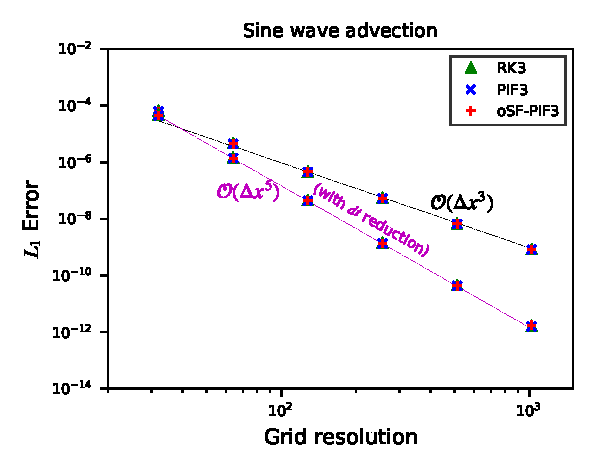
\includegraphics[width=0.85\textwidth]{fig/sine_over_dtReduction}
    \caption{Convergence test for the 1D sine wave advection problem.
        The errors are calculated
        in \( L_{1} \) sense against the initial density profile
        resolved on the computational grids refined
        from 32 to 1024 by a factor of 2.
        All numerical solutions follow the theoretical third-order convergence rate
        (the black-dotted line) when using the timesteps 
        computed from the Courant condition.
        Also plotted are the solutions of using reduced timesteps, which follows the
        fifth-order convergence rate represented in the pink-dotted line.
    }\label{fig:sine_wave}
\end{figure}

The simulation domain is defined on a one-dimensional box of \( [0, 1] \)
with the periodic boundary condition on both ends.
The density profile will propagate one period through the computational domain
and will return to its initial position at \( t = 1 \).
In return, any shape deformation of the density profile
from the initial density profile can be considered as a numerical error
associated with phase errors or numerical diffusions.
The accuracy of the numerical solutions is measured by computing \( L_{1} \) error
between the initial and the final density profiles.
The numerical experiment results from the sine wave advection test
on different number of grid points, \( N_{x} = 32, 64, 128, 256, 512, \) and \( 1024 \)
are depicted in~\cref{fig:sine_wave} for three different temporal methods, Rk3, PIF3, and oSF-PIF3.

There are two types of convergence rates demonstrated in~\cref{fig:sine_wave}.
In the first type, the numerical solutions of three different temporal methods
advanced with timesteps computed from the Courant condition with \( C_{\text{cfl}} = 0.7 \).
Interestingly, the numerical solutions from all three different temporal methods
show a third-order convergence rate, indicating that the leading error term from
third-order temporal methods dominates the spatial error from the fifth-order WENO-JS method.
These results are different from~\cref{fig:vortex_error_saturation},
calculating \( L_{1} \) error from the 2D nonlinear vortex advection case,
where the solution accuracy follows the spatial order at low-resolution regions
until the leading error of the solution is caught up by the temporal error
as computational grids get further refined to higher resolutions.
However, in this test case, the third-order temporal accuracy quickly takes control
throughout the entire range of the grid resolutions tested herein.
This solution behavior strongly supports the importance of
integrating spatially reconstructed solutions with a temporal scheme whose accuracy is
sufficiently high enough to be well comparable to that of the spatial solver.

In the second type of the convergence rate, on the other hand, the timesteps are restricted
in order to match up the lower third-order temporal accuracy with the higher fifth-order spatial accuracy.
Following the usual trick of timestep reduction in~\cite{mignone2010high},
the timestep \( \Delta t_{N} \) is manually adjusted on a grid size of \( N \)
to satisfy the equal rate of change between the spatial and temporal variations.
The restricted timestep is defined by,
\begin{equation}\label{eq:dt_reduction}
    {\Delta t_N} = {\Delta t_0} \Big( \frac{\Delta x_N}{\Delta x_0} \Big)^{\frac{5}{3}},
\end{equation}
where the sub-indices ``0'' and \( N \) refer to the time and grid scales
on a nominal coarse and fine resolution, respectively.
In the current configuration, \( \Delta x_{0} \) is the grid-scale of \( N_{x} = 32 \),
and \( \Delta t_{0} \) is the corresponding timestep subject to the Courant condition with \( C_{\text{cfl}} = 0.7 \).
With the timestep reduction, the overall leading error from the spatial and temporal methods
are matched with the fifth-order spatial accuracy of WENO5,
and the numerical solution of PIF3 and oSF-PIF3 follows the fifth-order convergence rate as expected.
In all test cases for linear advection problems, the oSF-PIF3 solutions behave
almost equally well with the solutions of the original PIF3 and RK3 both quantitatively and qualitatively.



\subsection{Nonlinear isentropic vortex advection}\label{subsec:vortex_weno}

The isentropic vortex advection problem~\cite{shu1998essentially} is one of the most popular benchmark tests
to measure the numerical method's accuracy and performance in the nonlinear case.
Although the problem is fully nonlinear, the exact solution always exists
in the form of its initial condition,
from which an isentropic vortex is advected through periodic boundaries in a 2D computational box.
The accuracy of a numerical method on a nonlinear problem
can be evaluated by comparing the final density profile with the initial condition.

The initial condition consists of a constant background mean flow with \( \rho = 1 \),
\( (u, v) = (1,1) \) and \( p =1 \) on the 2D computaional domain
with periodic boundary conditions.
The isentropic vortex is given by the velocity perturbations \( (\delta u, \delta v) \),
and the temperature perturbation \( \delta T \).
The perturbation terms are designed to set the constant entropy \( S \)
everywhere in the simulation domain, i.e., \( \delta S = 0 \).
The perturbations are given as,
\begin{equation}\label{eq:isentropic_vortex_initial}
    \left( \delta u, \delta v \right) = \frac{\epsilon}{2 \pi} e^{-\half \left( 1 - r^{2} \right)} (-y, x), \quad
    \delta T = - \frac{\left( \gamma - 1 \right) \epsilon^{2}}{8 \gamma \pi^{2}} e^{1 - r^{2}},
\end{equation}
where \( \epsilon = 5 \) is the vortex strength and \( r^{2} = x^{2} + y^{2} \).
The vortex is initially located at the domain center,
and it advects to the diagonal directions, then returns to its original position after one cycle.
The simulation domain size is doubled-up as \( [0, 20] \times [0, 20] \)
compared to the original setup in~\cite{shu1998essentially},
to prevent vortex-vortex couplings near the periodic boundaries
as reported in~\cite{spiegel2015survey}.

\begin{figure}
    \centering
    \begin{subfigure}{70mm}
        \centering
        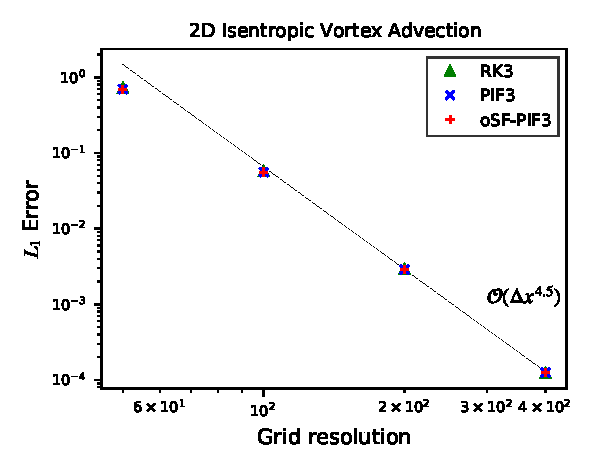
\includegraphics[width=0.95\textwidth]{fig/vortex_third}
    \end{subfigure}
    \begin{subfigure}{70mm}
        \centering
        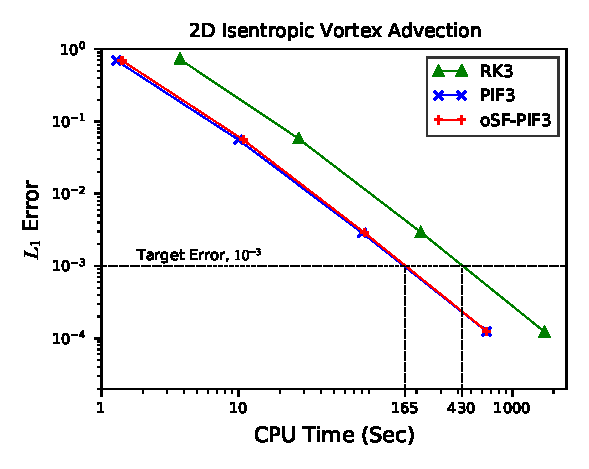
\includegraphics[width=0.95\textwidth]{fig/vortex_time_third}
    \end{subfigure}
    \caption{The \( L_{1} \) errors of the isentropic vortex advection test problem
        on different grid resolutions, \( N_{x} = N_{y} = 50, 100, 200, \) and \( 400 \).
        The three different third-order temporal schemes
        are used combined with WENO5 spatial method.
        The \( L_{1} \) errors
        with respect to the grid resolutions (\textbf{left});
        with respect to the computation time (\textbf{right}).
    }\label{fig:vortex_third}
\end{figure}

The results of the convergence test are depicted on the left panel in~\cref{fig:vortex_third}.
Three different temporal schemes, RK3, PIF3, and oSF-PIF3, show an excellent comparable match in
magnitudes and slopes of the \( L_{1} \) errors with varying grid resolution, \( N_{x} = N_{y} = 50, 100, 200, \) and \( 400 \).
One important finding in this figure is that there is no significant distinction
between PIF3 and oSF-PIF3 in accuracy and performance.
These results demonstrate that the original SF method
does not affect the solution accuracy and performance of the PIF method.

\begin{table}
    \centering
    \caption{The \( L_{1} \) errors, the rates of convergence,
        and the relative computation times for the vortex advection test.
        Here, the comparison between RK3 and oSF-PIF is only displayed,
        since the difference between oSF-PIF3 and PIF3 is indistinguishable.
        All the performance results (measured in seconds) are averaged
        over 10 simulation runs which are conducted on
        a Coffee Lake quad-core i7 Intel CPU with a
        clock speed of 2.7GHz, Turbo Boost up to 4.5GHz,
        utilizing four parallel threads.
    }\label{table:vortex_weno_third}
    \begin{adjustbox}{width=\textwidth}
        \begin{tabular}{@{}lcccclcccc@{}}
            \toprule
            \multirow{2}{*}{\( N_{x} = N_{y} \)} & \multicolumn{4}{c}{RK3} &  & \multicolumn{4}{c}{oSF-PIF3} \\
            \cmidrule(lr){2-5} \cmidrule(l){7-10}
            & \(L_{1}\) error & \(L_{1}\) order & CPU Time & Speedup &  &
            \(L_{1}\) error & \(L_{1}\) order & CPU Time & Speedup \\ \midrule
            50  & \num{7.22E-1} & \--- & \SI{3.73}{\second}    & 1.0 &  & \num{6.95E-1} & \--- & \SI{1.41}{\second} & 0.38 \\
            100 & \num{5.76E-2} & 3.65 & \SI{27.51}{\second}   & 1.0 &  & \num{5.58E-2} & 3.64 & \SI{10.82}{\second} & 0.39 \\
            200 & \num{2.94E-3} & 4.29 & \SI{214.44}{\second}  & 1.0 &  & \num{2.89E-3} & 4.27 & \SI{83.21}{\second} & 0.39 \\
            400 & \num{1.22E-4} & 4.59 & \SI{1727.71}{\second} & 1.0 &  & \num{1.26E-4} & 4.52 & \SI{652.18}{\second} & 0.38
        \end{tabular}
    \end{adjustbox}
\end{table}

The performance results of three different temporal schemes are presented
on the right panel of~\cref{fig:vortex_third} and summarized in~\cref{table:vortex_weno_third}.
Both the PIF3 and oSF-PIF3 methods perform more than two times faster than the multi-stage method, RK3.
It is worth noting that the original SF-PIF method, oSF-PIF, can be readily swappable
with an RK integrator in an existing code without too much effort,
leaving any existing spatial implementations intact.
Moreover, such a code transformation with oSF-PIF is more advantageous in simplicity
than the original PIF method because oSF-PIF replaces the analytic derivations of the Jacobian and Hessian terms
with the system-free approximations,
which have shown to be highly commensurate with
the analytical counterparts of the original PIF scheme.

Unlike the 1D linear sine advection test in~\cref{subsec:sine_wave},
the overall solution accuracy is not completely dominated by the third-order temporal discretizations,
which could reduce the overall convergence rate down to third-order as observed in the sine advection case.
Concurrently, the solution does not converge at full fifth-order either,
the rate due to the use of WENO5.
This can be explained as a nonlinear effect in which the lower third-order time integration schemes
slightly compromise the overall leading error term of the fifth-order spatial discretization.

\begin{figure}
    \centering
    \begin{subfigure}{70mm}
        \centering
        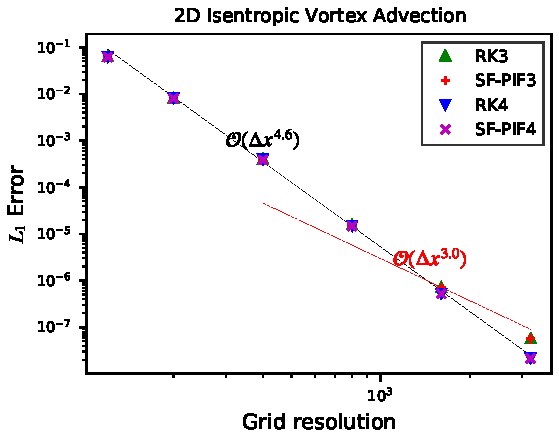
\includegraphics[width=0.95\textwidth]{fig/weno5_vortex_error_fourth}
    \end{subfigure}
    \begin{subfigure}{70mm}
        \centering
        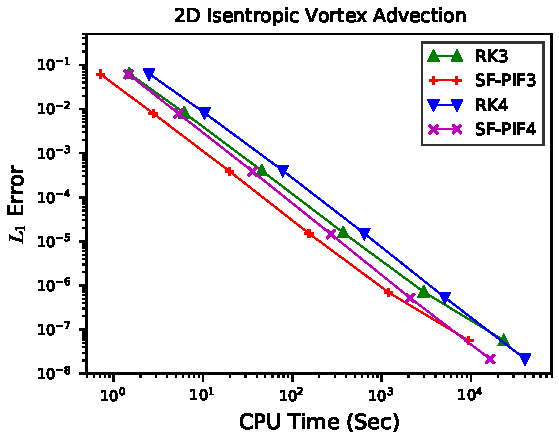
\includegraphics[width=0.95\textwidth]{fig/weno5_vortex_time_fourth}
    \end{subfigure}
    \caption{The \( L_{1} \) errors of the isentropic vortex advection test problem
        solved by third- and fourth-order temporal schemes combined with WENO5 spatial method.
        The \( L_{1} \) errors
        with respect to the grid resolutions (\textbf{left});
        with respect to the computation time (\textbf{right}).
    }\label{fig:vortex_fourth}
\end{figure}

However, the third-order temporal schemes gradually degrade the overall solution accuracy
on the fine grid resolutions. \cref{fig:vortex_fourth} illustrates the same convergence test results,
but in this case, containing more higher grid resolutions, \( N_{x} = N_{y} = 120, 200, 400, 800, 1600, \) and \( 3200 \).
Notice that the recursive SF-PIF method, SF-PIF3, and SF-PIF4 are used instead of the original SF-PIF method.
As expected, all temporal methods follow the convergence line of order \( \sim \mathcal{O}(\dx^{4.5}) \),
which is nearly the same as WENO's fifth-order spatial accuracy, equivalently in~\cref{fig:vortex_third}.
However, at the critical grid resolution, \( N_{x} = N_{y} = 1600 \),
the third-order temporal schemes of RK3 and SF-PIF3 start to compromise the overall solution accuracy.
This behavior can be explained that the spatial errors from the fifth-order WENO method
are dominant on the grid resolutions up to \( N_{x} = N_{y} = 1600 \),
after which the truncation errors associated with the third-order temporal methods
become dominant over the error of the fifth-order spatial solver, WENO5.
This result emphasizes the importance of high-order temporal methods in fine grid resolution:
a high-order spatial method does require a \textit{comparably} high-order temporal method
to maintain the overall quality of the solutions,
mainly when adding more grid resolutions to resolve finer scales more accurately.
Otherwise, lower-order accuracy from the temporal solver can potentially degrade
the solution accuracy, contradicting the intended motivation.

\begin{table}
    \centering
    \caption{The \( L_{1} \) errors, the rates of convergence,
        and the computation times for the vortex advection test
        solved using RK3 and SF-PIF3 methods (\textbf{top});
        using RK4 and SF-PIF4 methods (\textbf{bottom}).
        All simulation runs are equipped with WENO5 spatial method,
        performed on the four 20-cores
        Cascade Lake Intel Xeon processors, utilized 64 parallel threads.
        CPU times are measured in seconds, averaged over 10 individual runs.
    }\label{table:vortex_weno_fourth}
    \begin{adjustbox}{width=\textwidth}
        \begin{tabular}{@{}ccccclcccc@{}}
            \toprule
            \multirow{2}{*}{\( N_{x} = N_{y} \)} & \multicolumn{4}{c}{RK3} &  & \multicolumn{4}{c}{SF-PIF3} \\
            \cmidrule(lr){2-5} \cmidrule(l){7-10}
            & \(L_{1}\) error & \(L_{1}\) order & CPU Time & Speedup &  &
            \(L_{1}\) error & \(L_{1}\) order & CPU Time & Speedup \\ \midrule
            120  & \num{6.31E-2} & \--- & \SI{1.50}{\second}      & 1.0 &  & \num{6.16E-2} & \--- & \SI{0.71}{\second}    & 0.48 \\
            200  & \num{8.20E-3} & 4.00 & \SI{6.17}{\second}      & 1.0 &  & \num{7.96E-3} & 4.00 & \SI{2.77}{\second}    & 0.45 \\
            400  & \num{4.02E-4} & 4.35 & \SI{45.44}{\second}     & 1.0 &  & \num{3.86E-4} & 4.37 & \SI{19.89}{\second}   & 0.44 \\
            800  & \num{1.57E-5} & 4.68 & \SI{372.47}{\second}    & 1.0 &  & \num{1.51E-5} & 4.68 & \SI{153.92}{\second}  & 0.41 \\
            1600 & \num{7.18E-7} & 4.45 & \SI{2957.26}{\second}   & 1.0 &  & \num{6.95E-7} & 4.44 & \SI{1203.10}{\second} & 0.41 \\
            3200 & \num{5.72E-8} & 3.65 & \SI{23274.37}{\second}  & 1.0 &  & \num{5.60E-8} & 3.63 & \SI{9494.65}{\second} & 0.41 \\
        \end{tabular}
    \end{adjustbox}
    \begin{adjustbox}{width=\textwidth}
        \begin{tabular}{@{}ccccclcccc@{}}
            \toprule
            \multirow{2}{*}{\( N_{x} = N_{y} \)} & \multicolumn{4}{c}{RK4} &  & \multicolumn{4}{c}{SF-PIF4} \\
            \cmidrule(lr){2-5} \cmidrule(l){7-10}
            & \(L_{1}\) error & \(L_{1}\) order & CPU Time & Speedup &  &
            \(L_{1}\) error & \(L_{1}\) order & CPU Time & Speedup \\ \midrule
            120  & \num{6.30E-2} & \--- & \SI{2.50}{\second}       & 1.0 &  & \num{6.14E-2} & \--- & \SI{1.47}{\second}     & 0.59 \\
            200  & \num{8.15E-3} & 4.00 & \SI{10.42}{\second}      & 1.0 &  & \num{7.91E-3} & 4.01 & \SI{5.33}{\second}     & 0.51 \\
            400  & \num{4.01E-4} & 4.35 & \SI{78.47}{\second}      & 1.0 &  & \num{3.85E-4} & 4.36 & \SI{35.89}{\second}    & 0.46 \\
            800  & \num{1.51E-5} & 4.73 & \SI{641.50}{\second}     & 1.0 &  & \num{1.46E-5} & 4.72 & \SI{270.94}{\second}   & 0.42 \\
            1600 & \num{5.33E-7} & 4.82 & \SI{5115.47}{\second}    & 1.0 &  & \num{5.21E-7} & 4.81 & \SI{2091.20}{\second}  & 0.41 \\
            3200 & \num{2.17E-8} & 4.62 & \SI{40195.034}{\second}  & 1.0 &  & \num{2.15E-8} & 4.60 & \SI{16377.73}{\second} & 0.41 \\
        \end{tabular}
    \end{adjustbox}
\end{table}

The performance results of recursive SF-PIF methods can be found
on the right panel of~\cref{fig:vortex_fourth} and \cref{table:vortex_weno_fourth}.
As shown in the right panel of \cref{fig:vortex_fourth},
the SF-PIF3 method is the fastest method in reaching any given target \( L_{1} \) error threshold until \( N_{x} = 1600 \).
However, on any grid resolutions finer than the critical resolution, \( N_{x} = 1600 \),
SF-PIF3's \( L_{1} \) error drops to the third-order convergence rate,
which ultimately crosses the straight convergence line of SF-PIF4.
SF-PIF3's error will remain larger than the errors from the fourth-order temporal methods
as long as the convergence rate follows the pattern at the high-resolution trail.

On the other hand, it is distinctively superior to see that SF-PIF4's solution
reaches any fixed target error in a \textit{faster} CPU time than the third-order RK3's solution
while keeping the numerical errors as low as RK4 results at all grid resolution tested herein.
Remark that \cref{table:vortex_weno_fourth} shows quantitatively that
the SF-PIF4 method performs \textit{faster} than the RK3 method,
producing more accurate solutions at any grid resolution.







\subsection{Sod shock tube problem}\label{subsec:sod}

The Sod's shock tube problem~\cite{sod1978survey} is the one of the most famous 1D hydrodynamics
test problems for testing a numerical scheme's capability to handle discontinuities and shocks.
The initial condition is given as,
\begin{equation}\label{eq:sod_init}
    \left( \rho, u, p \right) = \begin{cases}
        \left( 1, 0, 1 \right) & \text{for } x \le 0.5, \\
        \left( 0.125, 0, 0.1 \right) & \text{for } x > 0.5,
    \end{cases}
\end{equation}
in a simulation box of \( [0, 1] \), with outflow boundary conditions
on both ends at \( x = 0 \) and \( x = 1 \).
This benchmark problem is an excellent practice to
test if the PIF and oSF-PIF methods can be capture the shock discontinuities
appropriately.

\begin{figure}
    \centering
    \begin{subfigure}{0.49\textwidth}
        \centering
        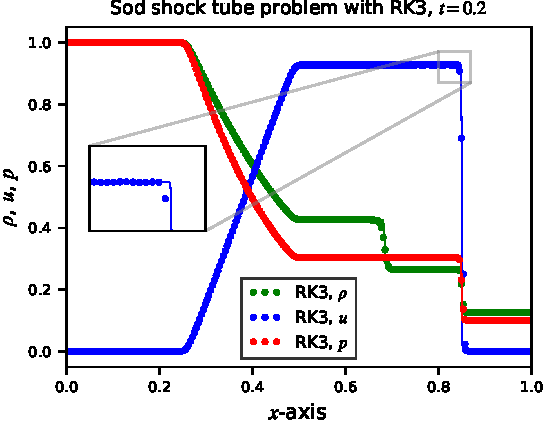
\includegraphics[width=\textwidth]{fig/sod_rk3}
        \caption{}\label{subfig:sod_rk3}
    \end{subfigure}
    \begin{subfigure}{0.49\textwidth}
        \centering
        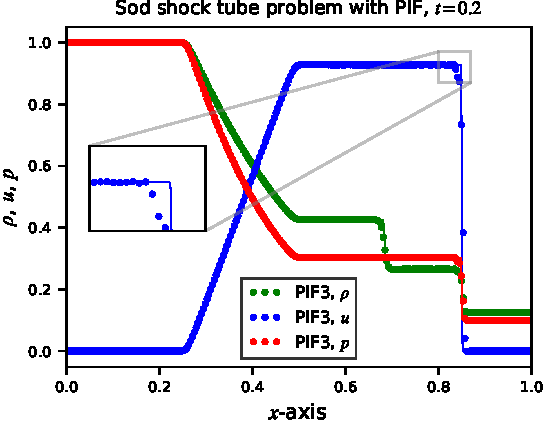
\includegraphics[width=\textwidth]{fig/sod_pif3}
        \caption{}\label{subfig:sod_pif3}
    \end{subfigure}
    \begin{subfigure}{0.49\textwidth}
        \centering
        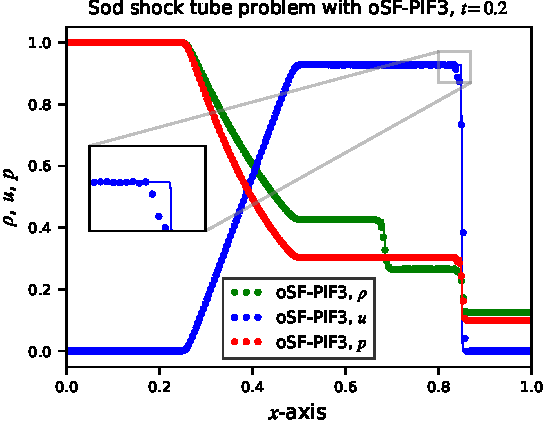
\includegraphics[width=\textwidth]{fig/sod_osf3}
        \caption{}\label{subfig:sod_osf3}
    \end{subfigure}
    \begin{subfigure}{0.49\textwidth}
        \centering
        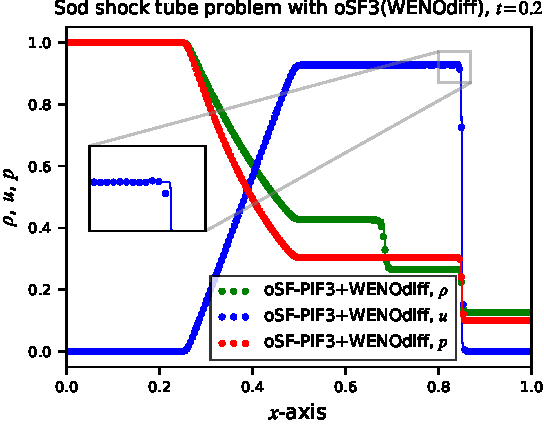
\includegraphics[width=\textwidth]{fig/sod_osf3_wenodiff}
        \caption{}\label{subfig:sod_osf3_wenodiff}
    \end{subfigure}
    \caption{Sod's shock tube problem at \( t = 0.2 \).
        The reference solutions are over-plotted
        as solid lines in each panel, which are resolved on a grid resolution of \( N_{x} = 1024 \)
        with RK3. The symbols in each panel represent the solution resolved on
        \( N_{x} = 256 \) grid cells with
        (\protect\subref{subfig:sod_rk3}) RK3,
        (\protect\subref{subfig:sod_pif3}) PIF3, and (\protect\subref{subfig:sod_osf3}) oSF-PIF3\@.
        (\protect\subref{subfig:sod_osf3_wenodiff}), the solution is resolved
        with oSF-PIF3 method combining with a new WENO-\textit{like} numerical differentiate operator,
        described as in~\crefrange{eq:pif_wenodiff_subs}{eq:pif_wenodiff_linear_weights}.
    }\label{fig:sod_third}
\end{figure}

The numerical solutions with the grid size of \( N_{x} = 256 \) at \( t = 0.2 \) are plotted
as symbols in each panel of~\cref{fig:sod_third}.
The solid lines on each panel represent the reference solution resolved on a more finer grid size,
\( N_{x} = 1024 \), by using WENO5+RK3.
The results resolved with recursive SF-PIF3 methods are omitted in this figure,
since the differences between SF-PIF3 and oSF-PIF3 are indistinguishable.

As illustrated in~\cref{subfig:sod_pif3} and~\cref{subfig:sod_osf3},
oSF-PIF3 method produce almost identical results of PIF3,
agreeing with the reference solutions and RK3's solutions in~\cref{subfig:sod_rk3}.
However, both in PIF3 and oSF-PIF3 methods,
there is a slight oscillation in the x-velocity immediately behind the shock front.
This small oscillation is originated from the use of
the conventional central differencing formulae in~\cref{eq:pif_central_dfdx}
for both oSF-PIF3 and PIF3.

The WENO-\textit{like} differencing strategy in~\crefrange{eq:pif_wenodiff_subs}{eq:pif_wenodiff_linear_weights}
can resolve this oscillation. As displayed in~\cref{subfig:sod_osf3_wenodiff},
the interchanging central differencing to WENO-differencing helps
to improve the performance of oSF-PIF3 at the shock,
suppressing the post-shock oscillations observed in~\cref{subfig:sod_pif3} and~\cref{subfig:sod_osf3}.
With this small fix, the oSF-PIF3 results are almost identical to the RK3 results in~\cref{subfig:sod_rk3}.
Computationally, the WENO-\textit{like} differencing adds extra floating-point operations,
which consequently slows down oSF-PIF's and SF-PIF's overall performance.
For this reason, the WENO-\textit{like} discretization was employed only
on the Sod's shock-tube test as a guide,
while it was opt-out on the rest of the test problems in this dissertation
where any unphysical has not been observed shock/discontinuity oscillations.


\subsection{Implosion test}\label{subsec:implosion}

The next problem to consider is the implosion test problem
introduced by Hui et al.~\cite{hui1999unified}.
An unsteady flow configuration is given as an initial condition which launches
a converging shock wave towards the domain center.
Following a more straightforward version by Liska and Wendroff~\cite{liska2003comparison},
the only right upper quadrant
of the original setup in~\cite{hui1999unified} is taken
as the simulation domain.
In this setup, the simulation is initialized on a region of a 2D square box,
\( \left[ 0, 0.3 \right] \times \left[ 0, 0.3 \right] \),
enclosed with reflecting walls,
in which case a converging shock wave is launched toward the lower-left corner
at $(x,y)=(0,0)$.
The initial shock wave bounces at the reflecting walls and produces a double Mach
reflection along two edges of $x=0$ and $y=0$.
Consequently, two jets are formed along the edges, moving toward the origin $(x,y)=(0,0)$ and collide
with each other. This two-jet collision then ejects a newly-formed jet into the diagonal direction
$x=y$. Reflecting shocks continuously interact with the diagonal jet, turning it into
a long and narrow shape over time. The observed structures of filaments and fingers
along with the diagonal jet and at its base are progressively intensified by the
Ritchmyer-Meshkov instability, a level of which depends sensitively on
numerical dissipation.

The shape of the jet is the key view point of
the implosion test since it is a good indicator of
a numerical method's symmetric property and numerical dissipation.
If the numerical scheme fails to maintain a high level of symmetry,
the jet will eventually be derailed off-diagonally and deformed over time.
Besides, an excess amount of numerical dissipation will
turn the jet into a less narrow and less elongated shape along the diagonal.

\begin{figure}
    \centering
    \begin{subfigure}{70mm}
        \centering
        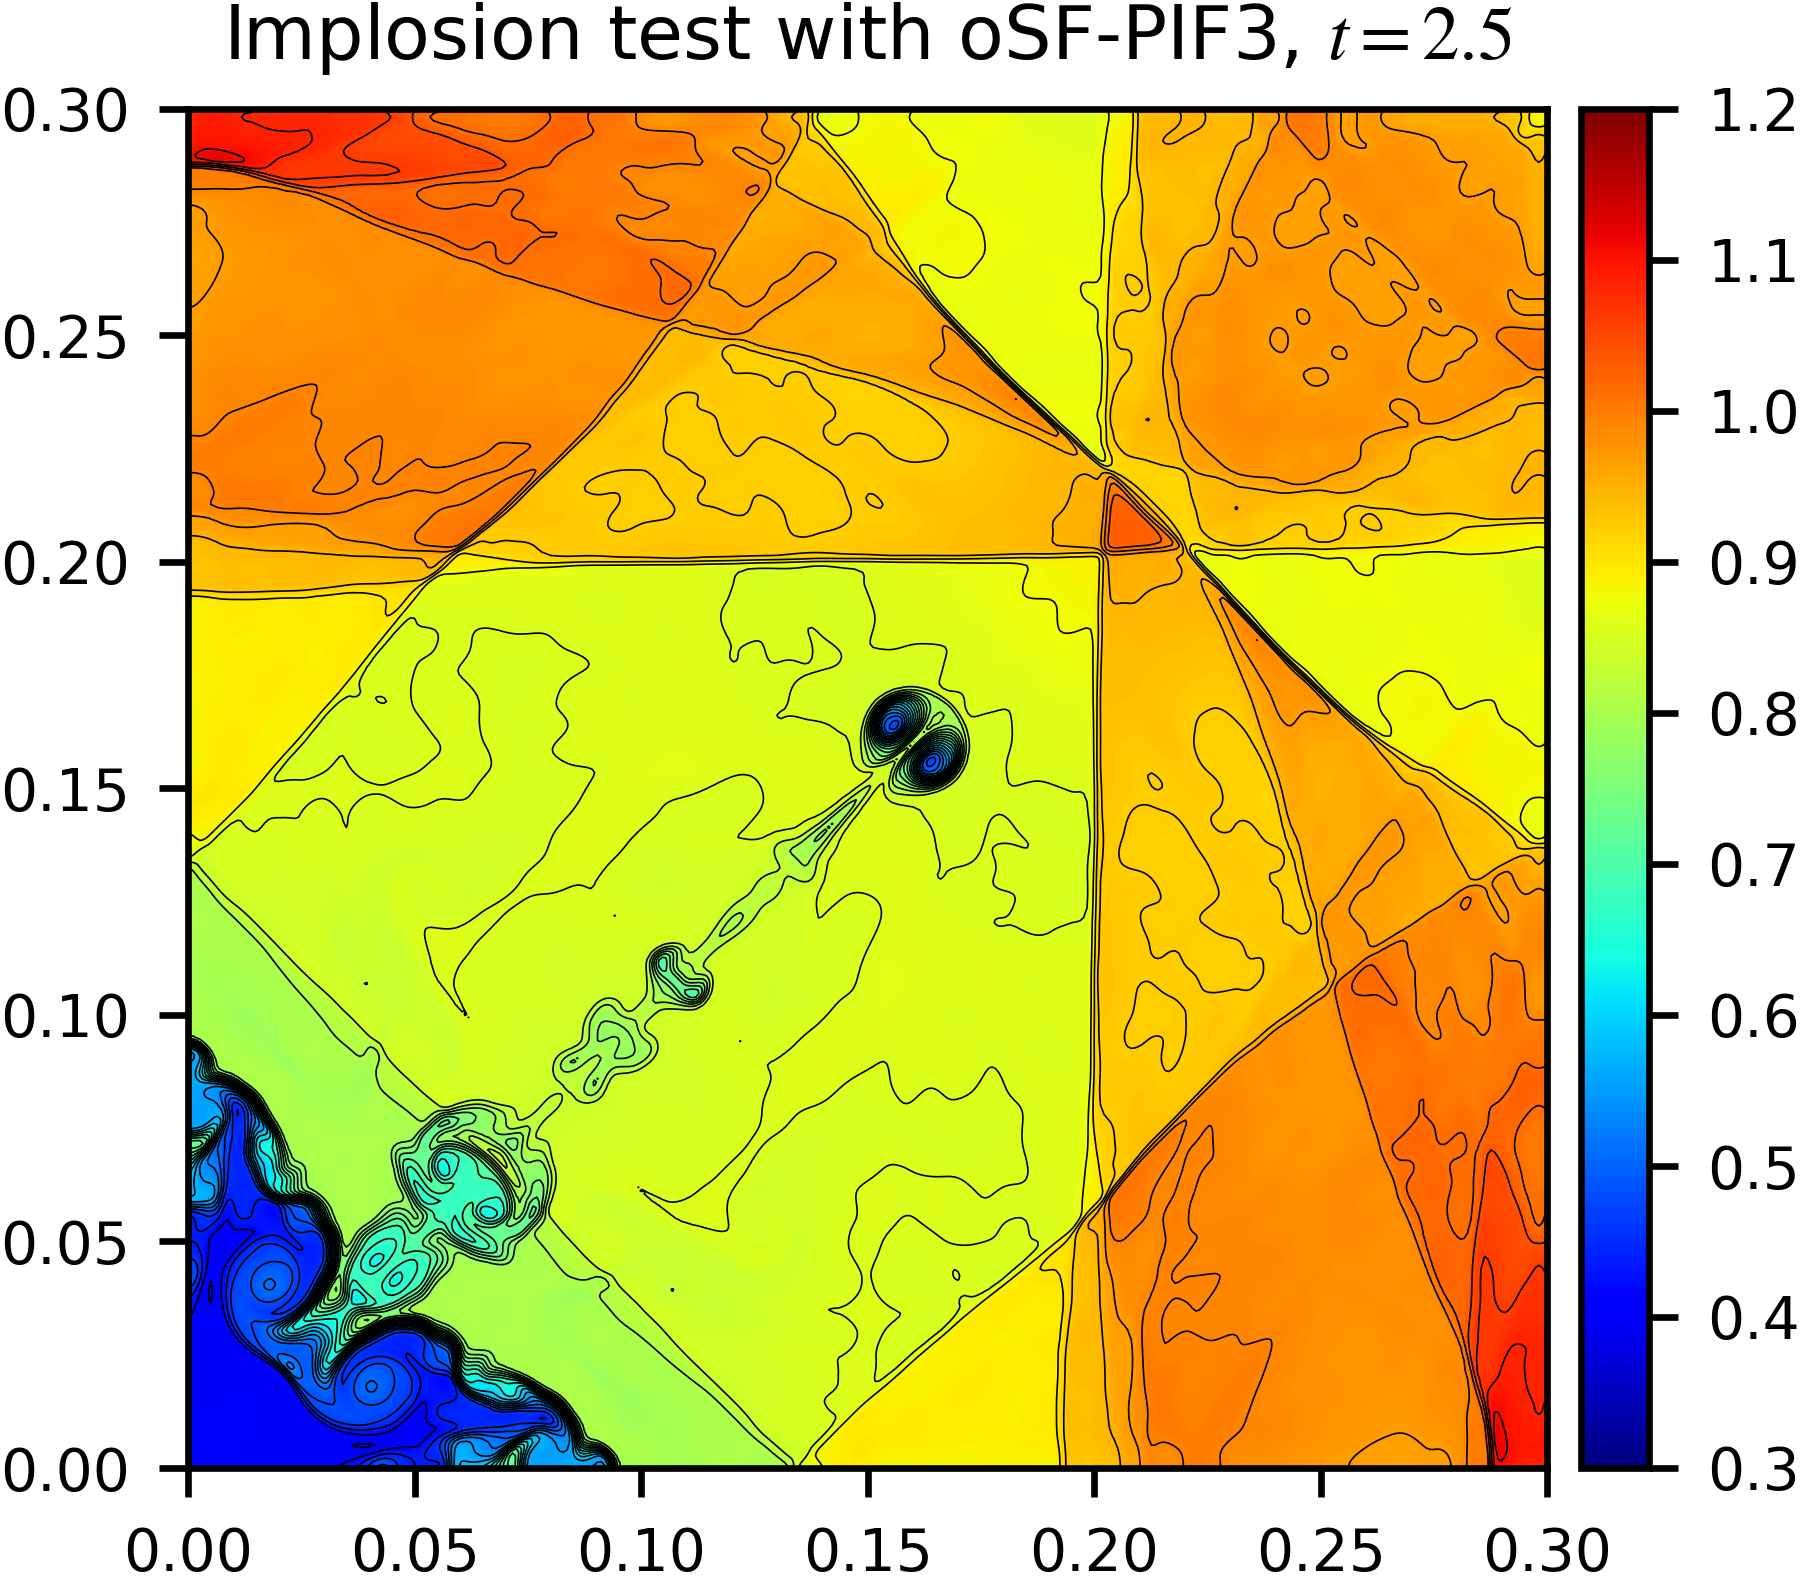
\includegraphics[width=0.95\textwidth]{fig/implosion_osf3.png}
    \end{subfigure}
    \begin{subfigure}{70mm}
        \centering
        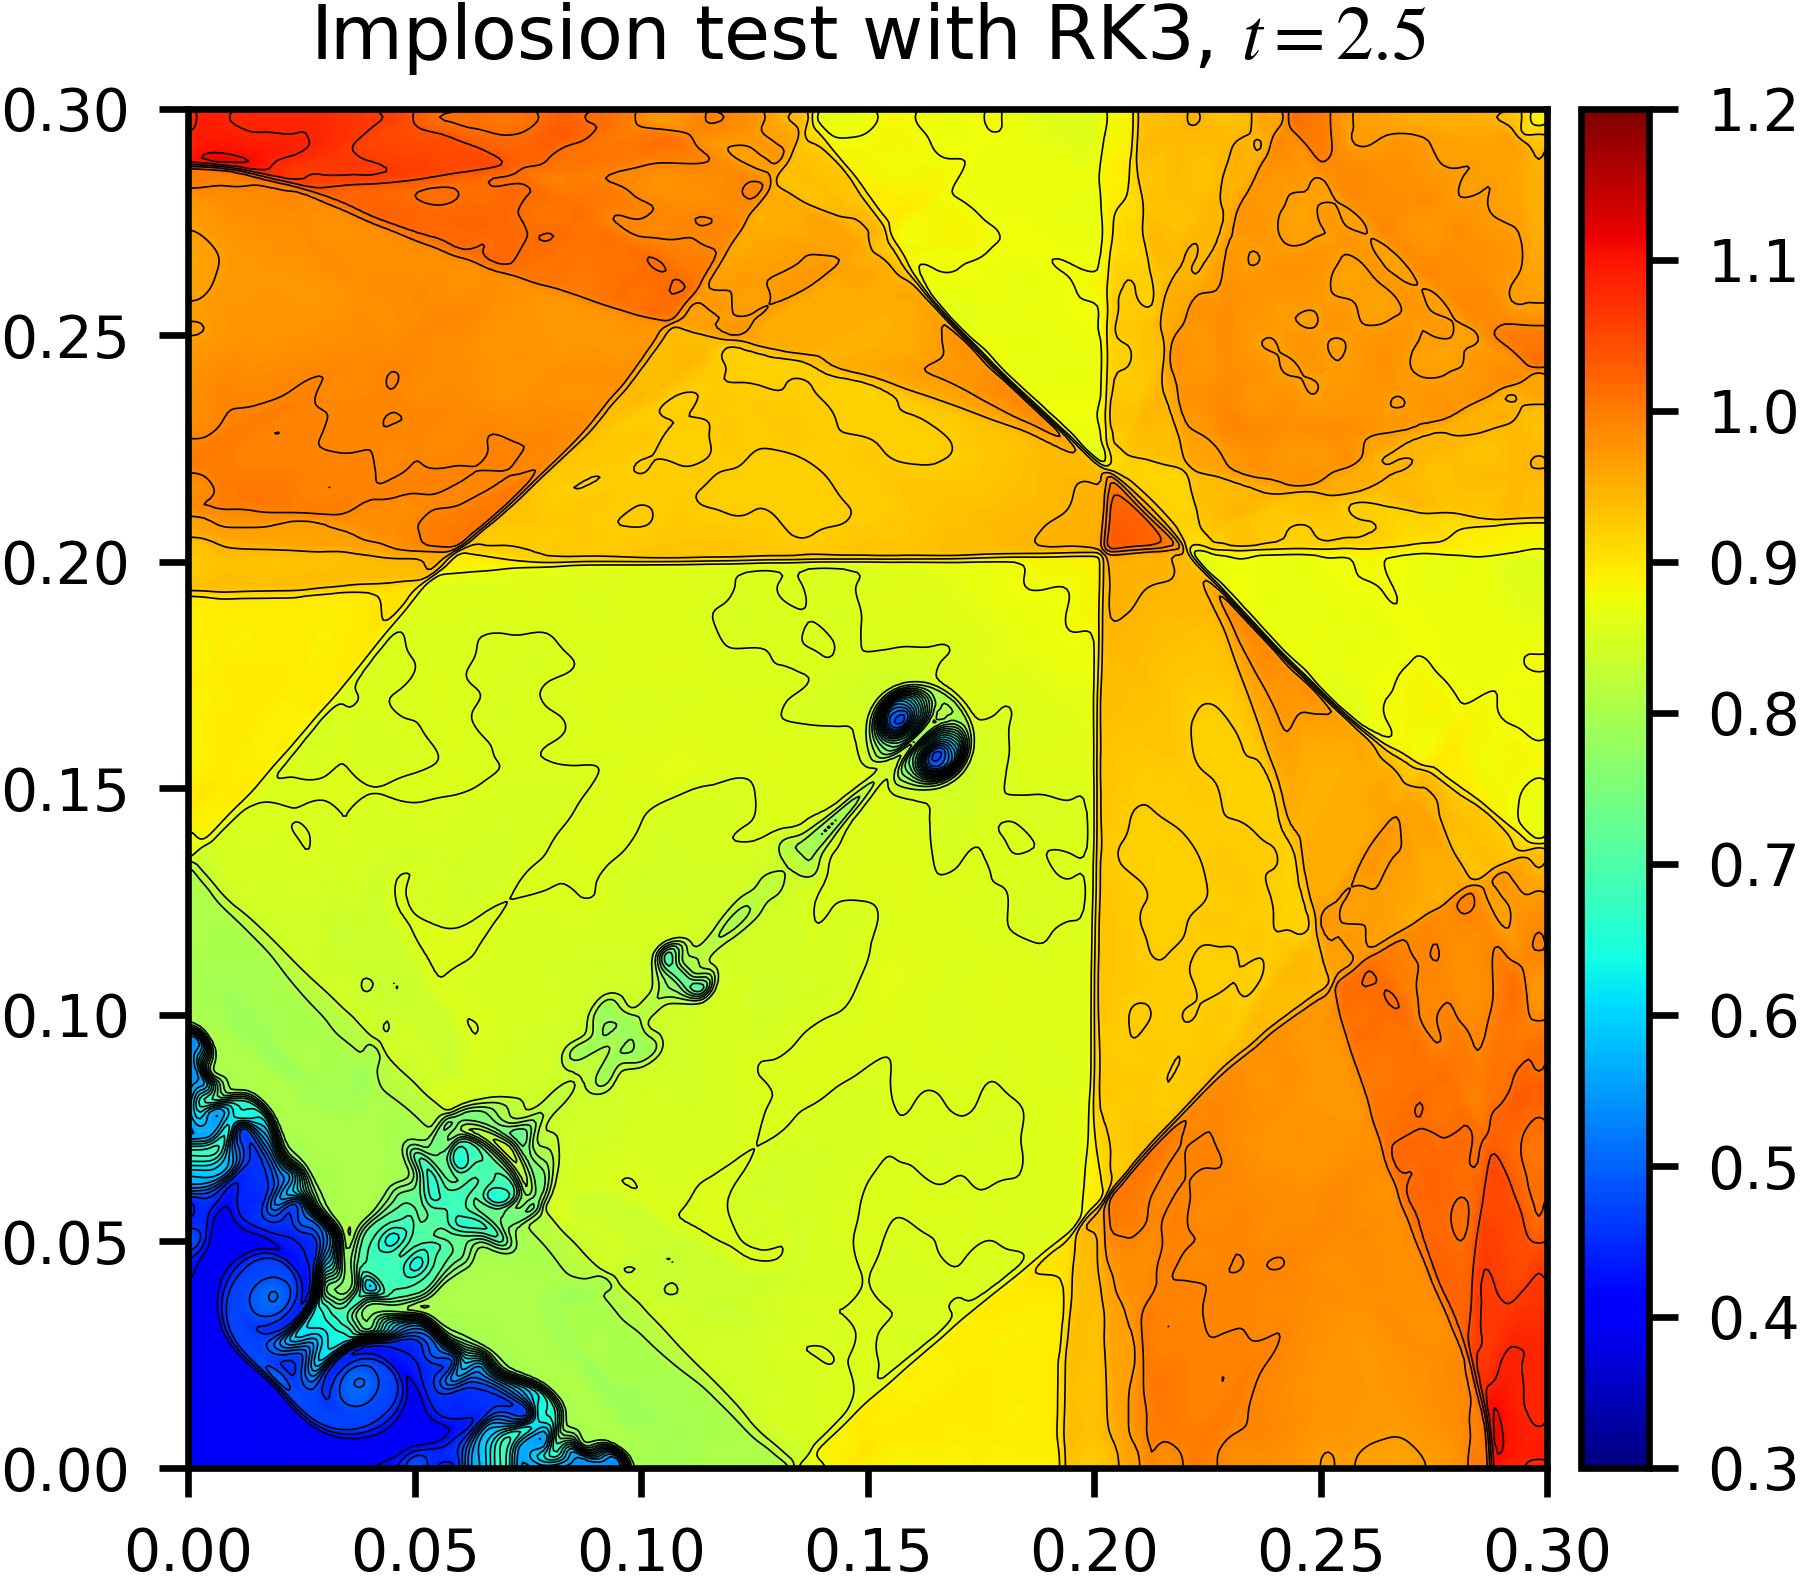
\includegraphics[width=0.95\textwidth]{fig/implosion_rk3.png}
    \end{subfigure}
    \caption{The density profile of the implosion test
        with oSF-PIF3 (left) and with RK3 (right).
        The color map ranges from \( 0.3 \) to \( 1.2 \), and
        40 evenly-spaced contour lines are over-plotted with
        the same range.
    }\label{fig:implosion}
\end{figure}

The density maps of the implosion test performed on
\( 400 \times 400 \) grid resolution at \( t = 2.5 \) are displayed in~\cref{fig:implosion}.
The result with oSF-PIF3 is on the left panel in \cref{fig:implosion} and RK3 on the right.
These results can also be directly compared with
Fig.~4.7 in~\cite{liska2003comparison} and Fig.~17 in~\cite{stone2008athena}.
The results of oSF-PIF3 (as well as RK3) present
the well-maintained symmetric jet along the diagonal direction
at a sufficient level.
At the same time, the shape of the diagonal jet using oSF-PIF3 matches
well with the shape using RK3,
and hence is sufficient to demonstrate that the numerical dissipation in oSF-PIF3
is well-managed compared with RK3.


\subsection{Shallow water equations}\label{subsec:shallow}

One of the essential features of the SF-PIF methods is that the SF-PIF methods
can be applicable to any other system without changing the high-order parts of the simulation codes.
As an example of the system independence feature,
the simulation result by changing the system of equations to the 2D shallow water equations (SWE)
without a source term is presented in this section.
In SWE, the conservative variables and the flux functions are defined by,
\begin{equation}\label{eq:swe_gov}
    \bU = \begin{bmatrix}
        h \\
        h u \\
        h v
    \end{bmatrix},\quad
    \bF (\bU) = \begin{bmatrix}
        h u \\
        h u^{2} + \frac{1}{2} g h^{2} \\
        h u v
    \end{bmatrix}, \quad
    \bG (\bU) = \begin{bmatrix}
        h v \\
        h u v \\
        h v^{2} + \frac{1}{2} g h^{2}
    \end{bmatrix}.
\end{equation}
Here, \( h \) is the vertical depth of the fluid,
\( \mathbf{v} = \left( u, v \right)  \) is a vector of 
vertically-averaged velocity components in $x$- and $y$-directions.
Denoted as \( g \) is a gravitational acceleration in the negative vertical 
$z$-direction, which is averaged out in the derivation of the shallow water equations.

The sole purpose of presenting the new system of equations above
is to demonstrate the flexibility of SF-PIF schemes,
in that the system-free approach allows an easy code implementation
without the need for other analytical derivations of new
Jacobian-\textit{like} terms of the new governing system.
By virtue of the system-independent property of the SF-PIF methods,
the process of changing from the 2D Euler code to the 2D SWE code is
no more than switching the governing equations
without touching anything on the high-order numerical parts.
This process is much simpler than other Lax-Wendroff type schemes (PIF, for example),
where each governing system should re-calculate the Jacobian-\textit{like} terms.

The well-known circular dam-breaking problem~\cite{alcrudo1993high,toro2001shock,delis2005numerical}
is conducted to validate the numerical capability of the SF-PIF method in SWE\@.
Initially, a volume of still water is confined
in the virtual (i.e., invisible) cylindrical 
wall with a radius of 11 meters (m),
located at the center of simulation domain,
\( \left[ \SI{50}{\meter} \times \SI{50}{\meter} \right] \)
resolved on a $100 \times 100$ grid resolution.
The depth of the water inside of the wall is
\( \SI{10}{\meter} \) and \( \SI{1}{\meter} \) outside.
This configuration would be considered as an
SWE version of 2D Riemann problem.
Explicitly, the initial condition is given as,
\begin{equation}\label{eq:swe-init}
    \left(h, u, v \right) = \begin{cases}
        \left(\SI{10}{\meter}, 0, 0 \right) & \text{for } r \le \SI{11}{\meter}, \\
        \left(\SI{1}{\meter}, 0, 0 \right) & \text{for } r > \SI{11}{\meter}, \\
    \end{cases}
\end{equation}
where \( r \) is the distance from the center of domain,
\( r = \sqrt{\left( x - \SI{25}{\meter} \right)^{2} + \left( y - \SI{25}{\meter} \right)^{2} } \).
The outflow boundary condition is applied for both directions,
and the gravitational acceleration is \( g = \SI{9.81}{\meter\per\square\second}\).
Again, the Courant number is set to \( C_{\text{cfl}} = 0.4 \).

\begin{figure}
    \centering
    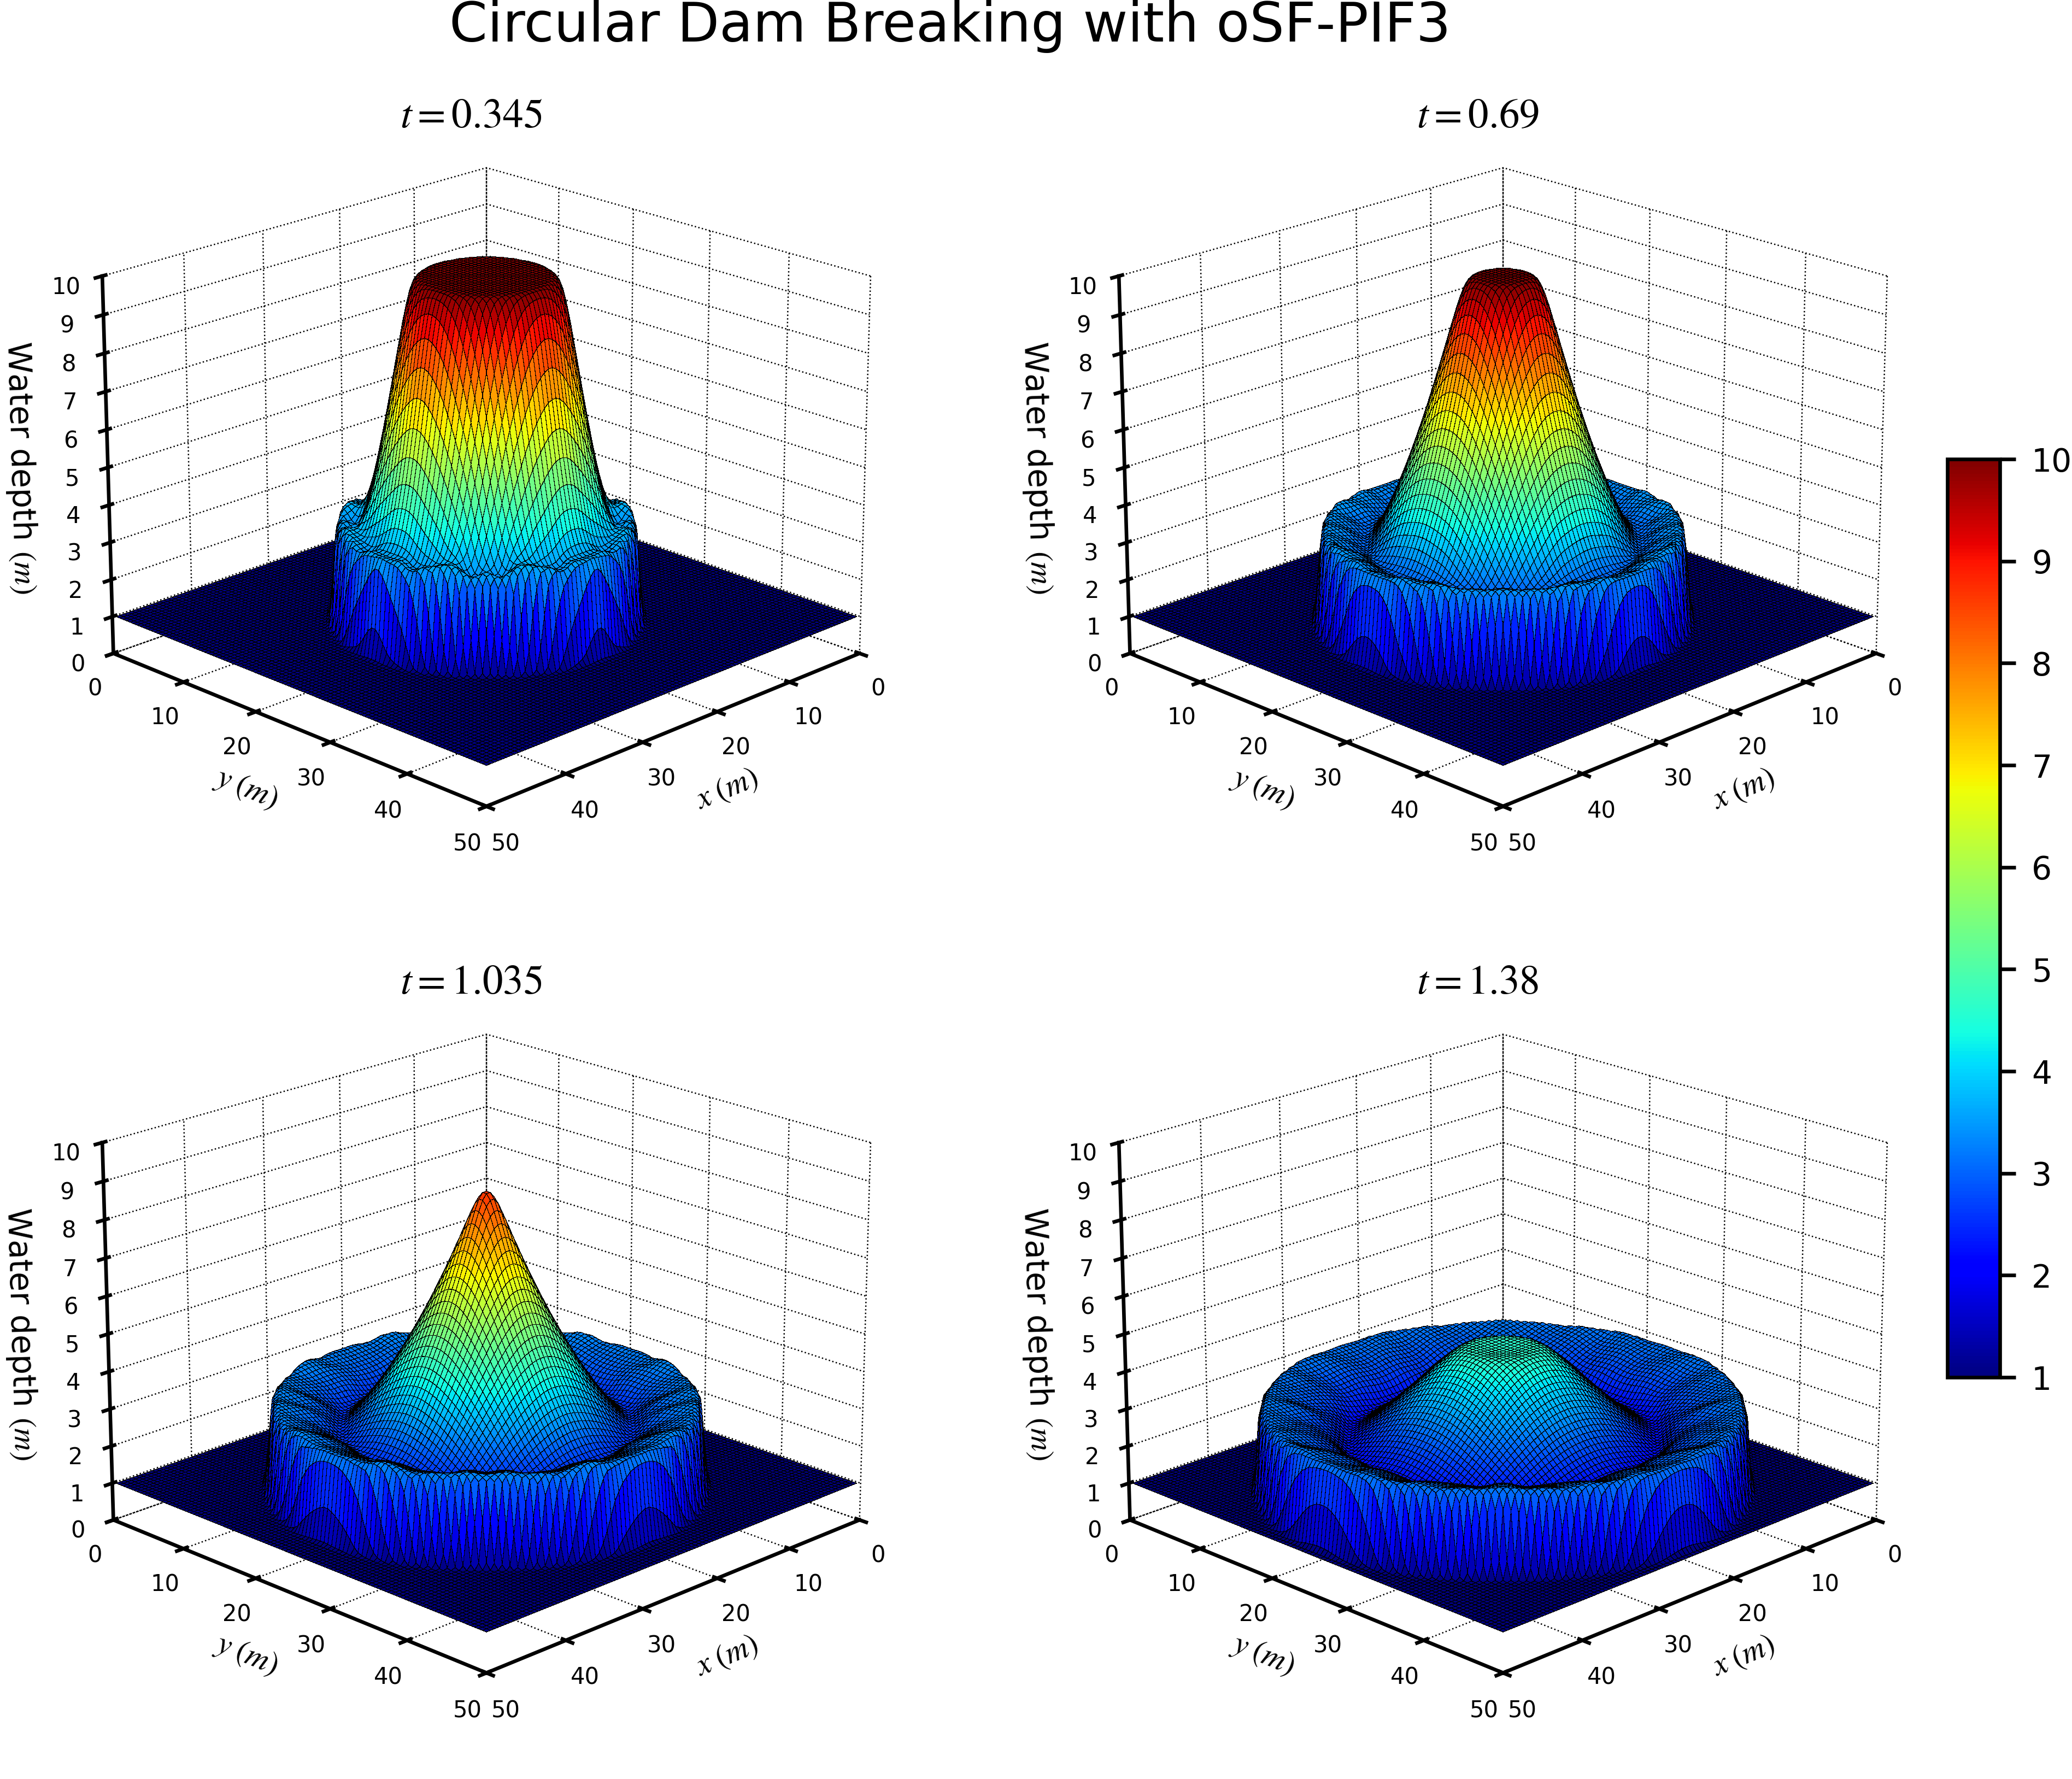
\includegraphics[width=\textwidth]{fig/swe_circ_osf3_all.png}
    \caption{Snapshots of the circular dam breaking simulation
        at four different times, \( t = 0.345, 0.69, 1.035, \) and $1.38$ seconds.
        A volume of water in rest is initially confined
        in a cylindrical dam of a radius $r=11$ m and a height $h=10$ m.
        The simulation starts with an instantaneous removal of the cylindrical wall
        located at the center of the domain
        \( \left[ \SI{50}{\meter} \times \SI{50}{\meter} \right] \)
        resolved on a grid resolution of $100 \times 100$.
        The gravitational force is exerted on the steady water,
        which triggers the onset of the gravitational collapse of the entire volume of water,
        making the circular splash in the outer rim as well as the ripple effects
        in the central region that move radially outward in time.
    }\label{fig:swe_circ}
\end{figure}

The results of the simulation with the oSF-PIF3 method are presented in~\cref{fig:swe_circ}.
The figure represents well-comparable numerical solutions
with the results using the same configuration
reported in~\cite{alcrudo1993high,toro2001shock,delis2005numerical}.
As shown in \cref{fig:swe_circ}, the overall spherical symmetry and the sharp profile
at the wavefront are well-maintained in each snapshot
at four different times, \( t = 0.345, 0.69, 1.035, \) and \( 1.38 \).



\section{SF-PIF method with WENO-JS}\label{sec:result_wenojs}

The previous section demonstrates that the original SF-PIF and recursive SF-PIF methods,
combined with the traditional WENO method,
generate the highly accurate and stable solution in faster computational time
compared to the SSP-RK methods.
This section provides numerical test results from additional benchmark problems,
both in 2D and 3D, with the presence of strong shock.
All simulations are performed with third-order and fourth-order \textit{recursive} SF-PIF methods
coupled with the traditional fifth-order WENO method described in~\cref{subsec:weno}.
2D simulations are carried out on high grid resolutions
to emphasize the numerical effects of the temporal solver, as discussed in~\cref{subsec:vortex_weno}.

\subsection{The Shu-Osher problem (rotated \(\ang{45}\))}\label{subsec:shu45_weno}

The Shu-Osher problem~\cite{shu1989efficient} is a well-known benchmark problem
that describes the interactions between a Mach 3 shock and a smooth density profile.
Initially, a Mach 3 shock wave travels to the right through a sinusoidally perturbed
density profile. As the shock wave propagates along the perturbed region,
the profile gets compressed, resulting in a frequency-doubled region behind the shock. 
As the shock wave moves further to the right,
the doubled-frequency region returns to its original frequency, at which point
it becomes a sequence of sharp profile instead of smooth sine wave
due to the shock-steepening.

In this section, the Shu-Osher problem is performed in 2D by inclining the shock wave direction
by an angle of \(\theta = \ang{45} \),
adopting the idea of Kawai~\cite{kawai2013divergence},
where the initial conditions are repeated multiple times along the direction of the
wave propagation so that the problem may be executed with periodic boundary conditions.
Explicitly, the initial condition is given as,
\begin{equation}\label{eq:shu45_gov}
    \begin{split}
        &\bU(x_{\parallel}, t=0) = \begin{cases}
            \bU_{L} & \text{for } x_{\parallel} \le 1, \quad 11 < x_{\parallel} \le 21, \quad 31 < x_{\parallel} \le 40, \\
            \bU_{R} & \text{for } 1 < x_{\parallel} \le 11, \quad 21 < x_{\parallel} \le 31,
        \end{cases}\\
        &\text{where } \bU_{L} = \begin{bmatrix}
            \rho = 3.857143 \\
            u = 2.629369\cos(\pi/4) \\
            v = 2.629369\sin(\pi/4) \\
            p = 10.33333
        \end{bmatrix},\quad
        \bU_{R} = \begin{bmatrix}
            \rho = 1 + 0.2\sin(5 x_{\parallel}) \\
            u = 0 \\
            v = 0 \\
            p = 1
        \end{bmatrix}.
    \end{split}
\end{equation}

\begin{figure}
    \centering
    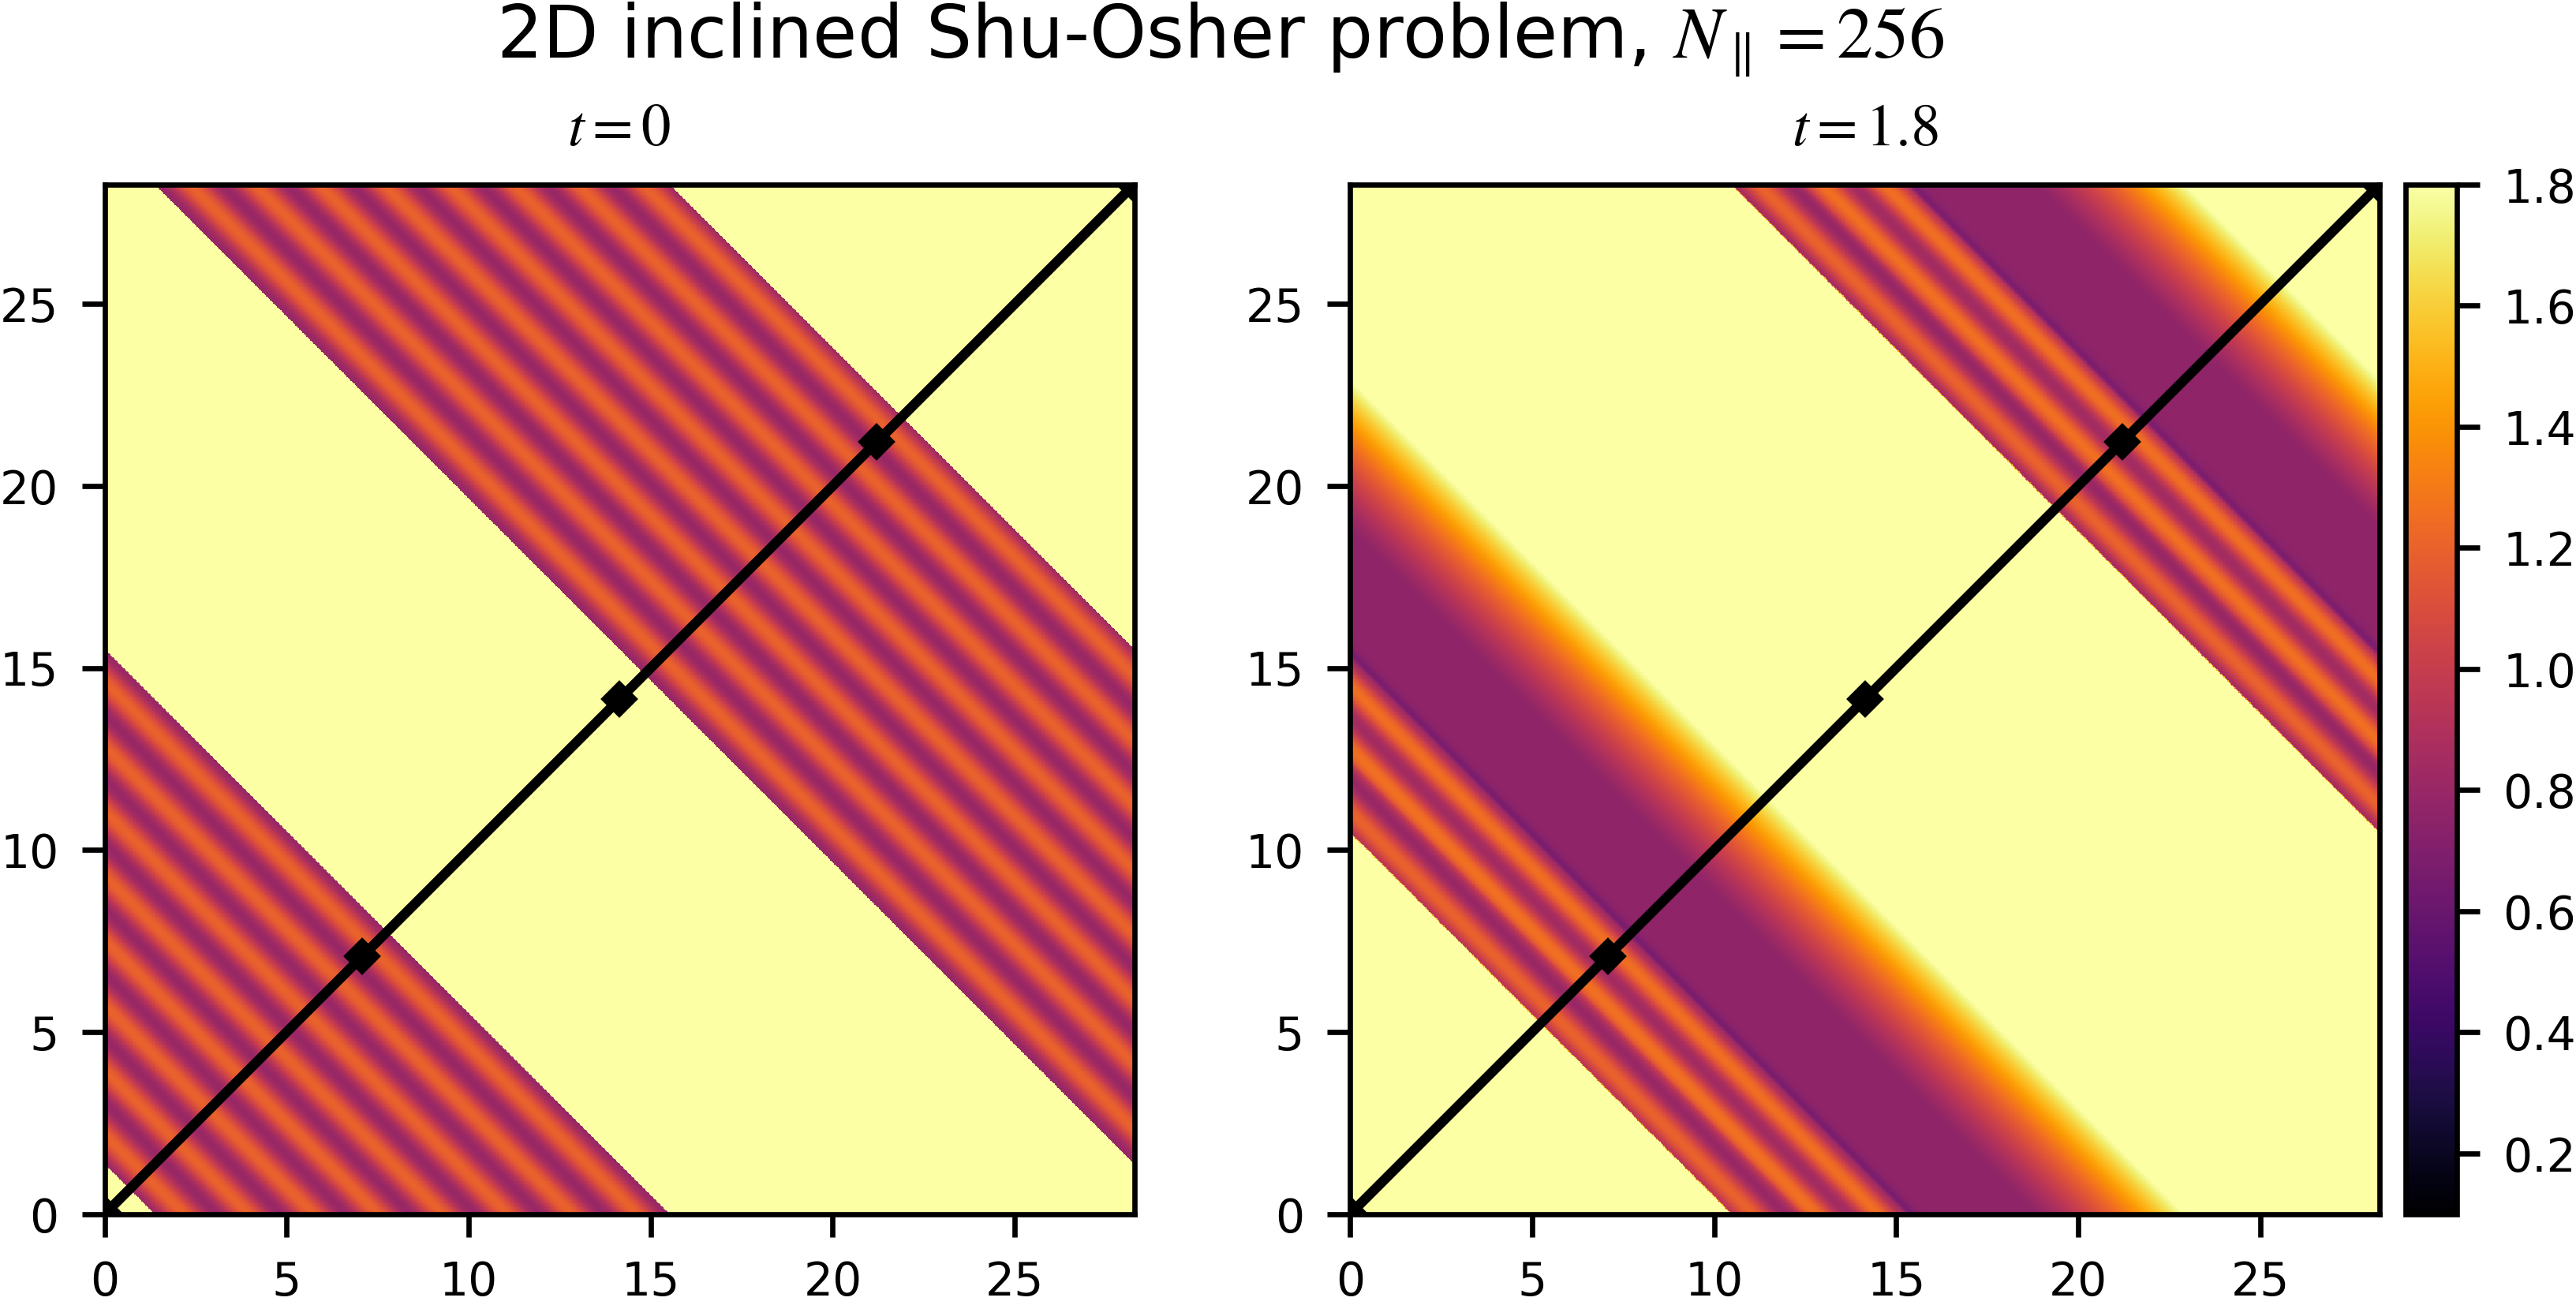
\includegraphics[width=0.95\textwidth]{fig/shu45_2d_snapshot.png}
    \caption{2D density maps of inclined 2D Shu-Osher test problem
        at \( t=0 \) and \( t=1.8 \). The test was performed on a 2D simulation box
        of \(1024 \times 1024 \) resolution with the SF-PIF4 method.
        The solid black line represents the shock propagating direction, \( x_{\parallel} \),
        and squares divide the line in each quartile.
    }\label{fig:shu45_cmap}
\end{figure}

\( x_{\parallel} = x \cos{\theta} + y \sin{\theta} \) is the direction
parallel to the wave propagation and the simulation domain is a periodic box of
\( [0, 20/\cos{\theta}] \times [0, 20/\sin{\theta}] \).
With this configuration, the 1D test problem, Shu-Osher test,
can be performed on the diagonal direction of 2D periodic box.
The same 1D solution is expected by following the diagonal direction, \( x_{\parallel} \),
and taking only the bottom-left quarter of the diagonal axis.
Therefore, the number of data points of this result profiles
would be a quarter of the 2D grid resolution,
i.e., \( N_{\parallel} = N_{x}/4 = N_{y}/4 \).
The 2D density map of the initial and final conditions are plotted in~\cref{fig:shu45_cmap}.

\begin{figure}
    \centering
    \begin{subfigure}{70mm}
        \centering
        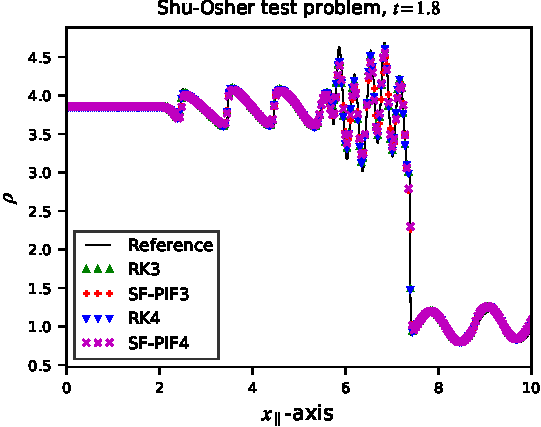
\includegraphics[width=0.95\textwidth]{fig/shu45_weno5_256}
    \end{subfigure}
    \begin{subfigure}{70mm}
        \centering
        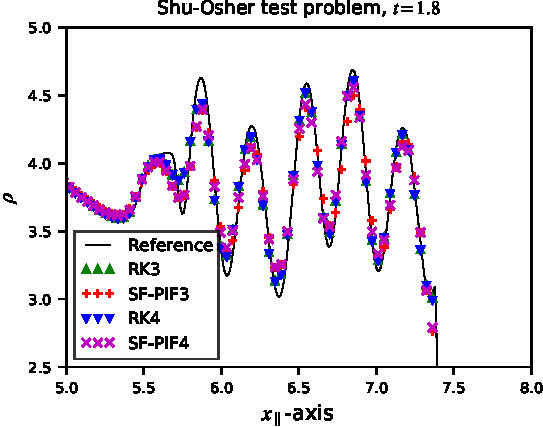
\includegraphics[width=0.95\textwidth]{fig/shu45_weno5_256_zoomed}
    \end{subfigure}
    \caption{One dimensional density profiles along the \( x_{\parallel} \) direction 
        of the inclined Shu-Osher problem at \( t = 1.8 \).
        The solid line represents the reference solution,
        solved by RK4 with 1024 data points
        in the diagonal axis, i.e., \( N_{\parallel} = 1024 \).
        All other solutions, represented by the symbols, are resolved on an
        \( N_{\parallel} = 256 \) grid resolution in the diagonal axis.
        The detailed view of the high-frequency region is shown
        on the right panel.
    }\label{fig:shu45}
\end{figure}

The density profiles of the bottom-left quarter of the diagonal axis \( x_{\parallel} \)
are given in~\cref{fig:shu45}. All tests are performed on a box of resolution \( N_{x} = N_{y} = 1024 \),
so the effective resolution of each profile is \( N_{\parallel} = 256 \),
except for the reference solution, which performed on a finer grid, \( N_{\parallel} = 1024 \).
The four different temporal methods, RK3, RK4, SF-PIF3, and SF-PIF4 produce
reasonably acceptable solution profiles capturing the high-frequency amplitudes
fairly well in the frequency-doubled region.
Generally, RK methods capture the amplitudes marginally better,
but in the left-most part of the double-frequency region, \( x \approx 5.8 \),
SF-PIF methods capture the highest peak of the amplitude better than
the RK methods near the transition between the frequency 
doubling and the shock steepened perturbations.




\subsection{2D Riemann problem: Configuration 3}\label{subsec:2drp_c3_weno}

The two-dimensional Riemann problem is a widespread benchmark problem to test
the methods' ability to capture the complex fluid structures in 2D.
This specific setup and other types of configurations have been
extensively studied in~\cite{zhang1990conjecture, schulz1993classification, schulz1993numerical}
and have been adopted as prevalent benchmark test problems.
This dissertation follows the initial condition of Configuration 3
described in~\cite{don2016hybrid,lee2017piecewise,lee2021single,lee2021recursive}.

The simulation domain is set on \( 1600 \times 1600 \) grid resolution,
which is generally considered as a very high resolution in 2D simulation.
This grid resolution choice is made based on the observation in~\cref{subsec:vortex_weno}
to ensure that the temporal errors are comparable to or dominant over the spatial errors;
thereby, the temporal error dominant results are anticipated that allows
to see the different behaviors of four different temporal solvers.

\begin{figure}
    \centering
    \begin{subfigure}{140mm}
        \centering
        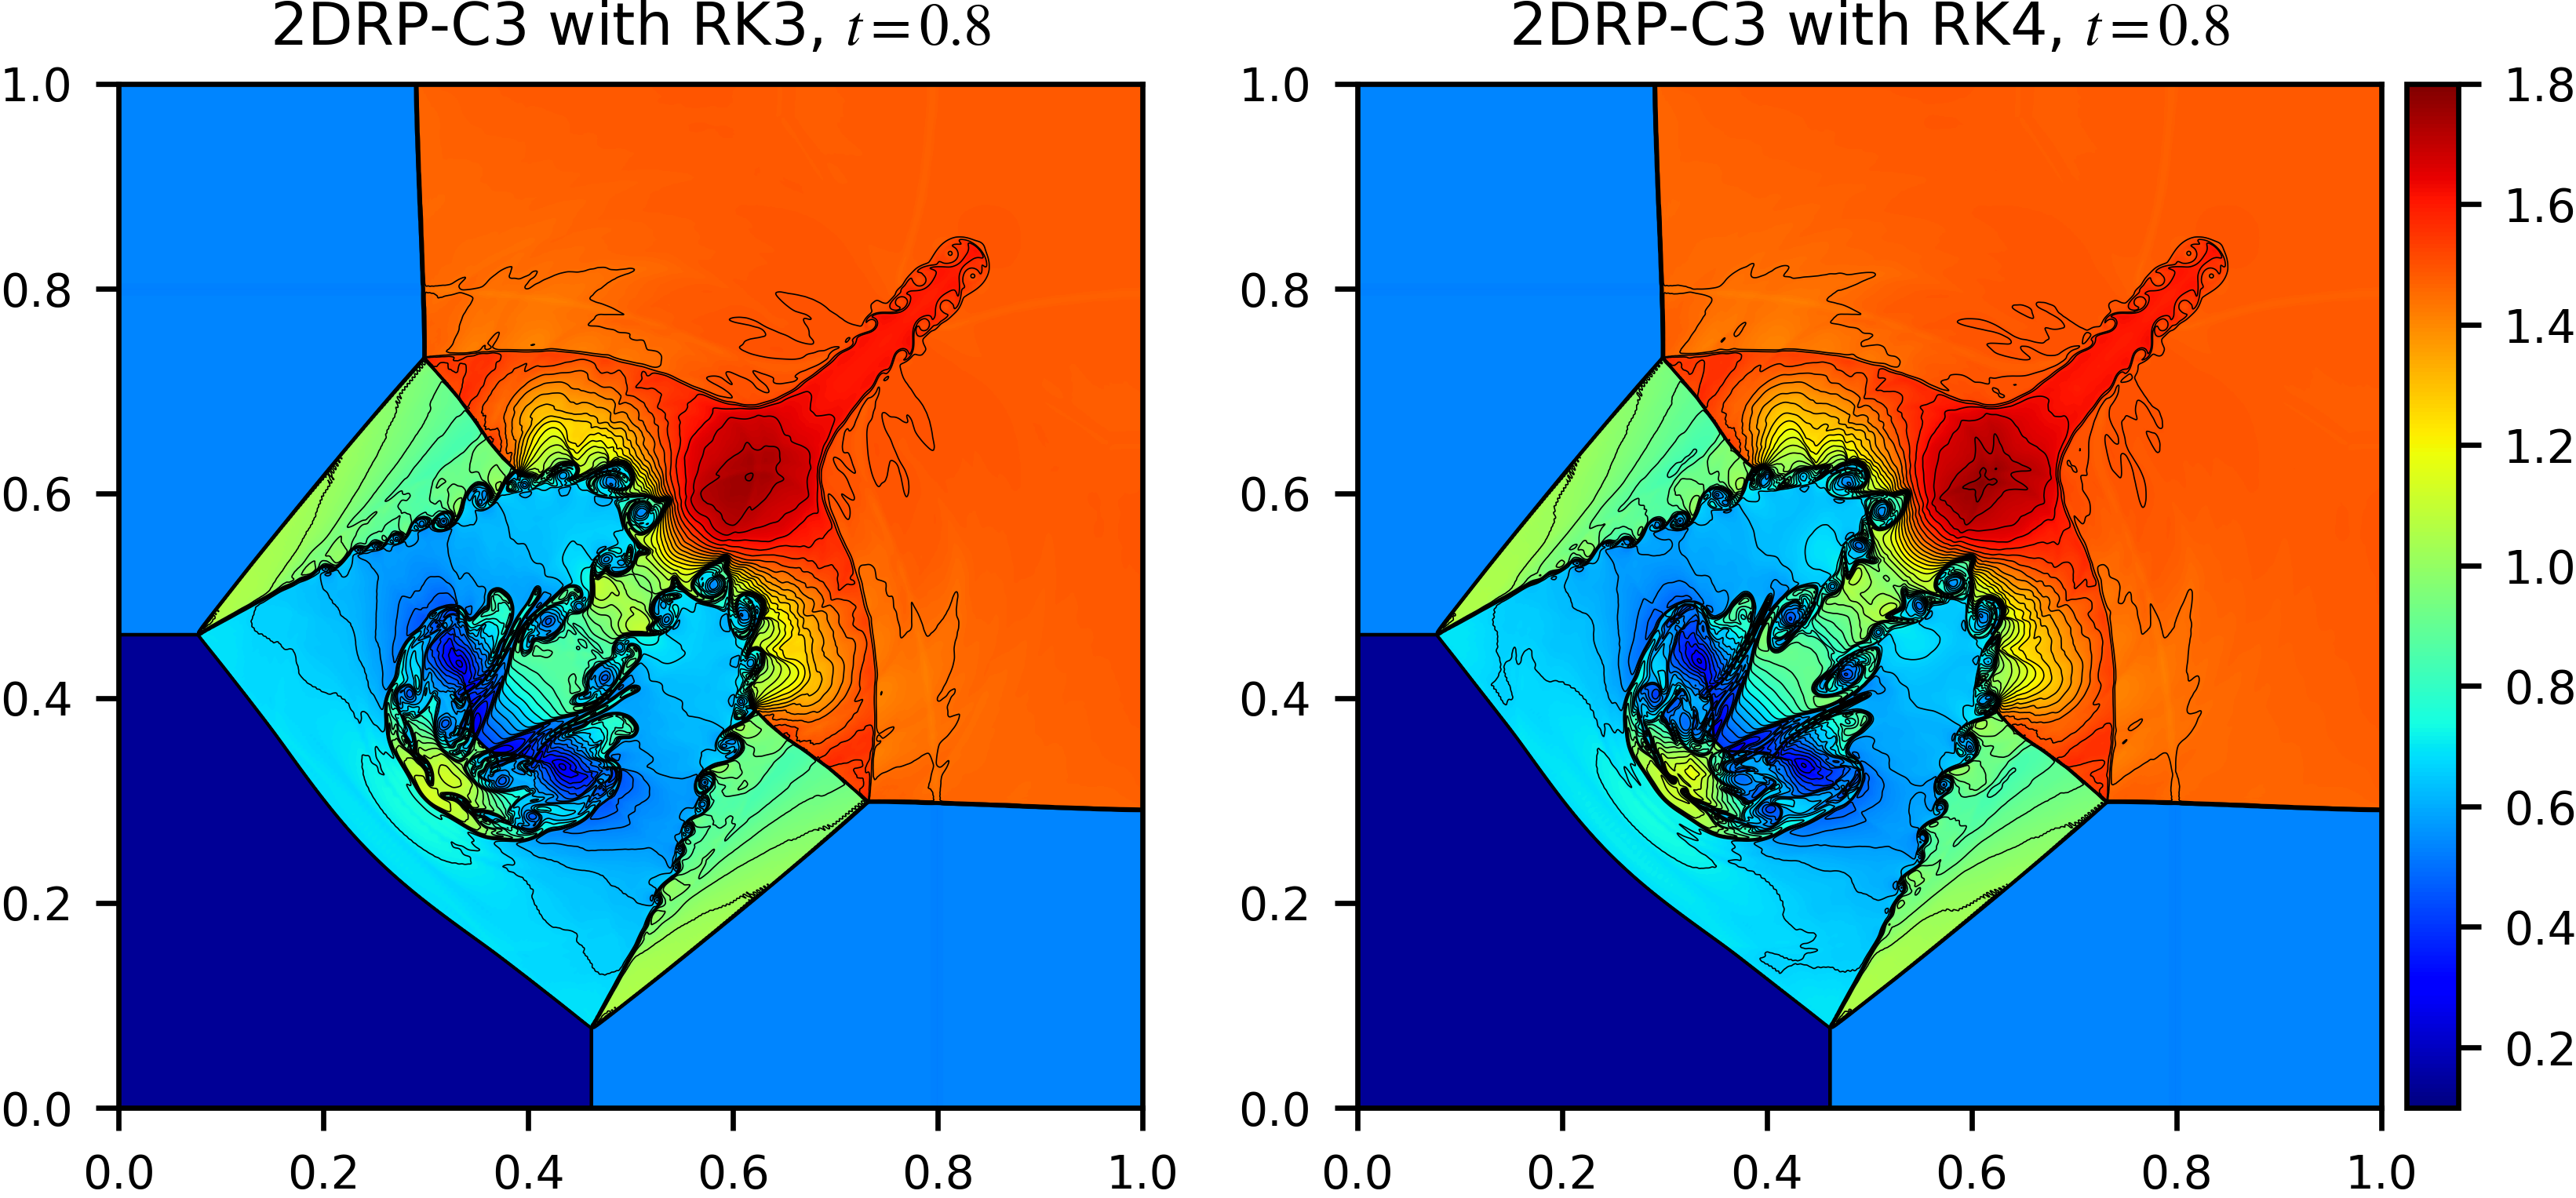
\includegraphics[width=0.9\textwidth]{fig/2drp_c3_weno5_rk_1600.png}
    \end{subfigure}
    \begin{subfigure}{140mm}
        \centering
        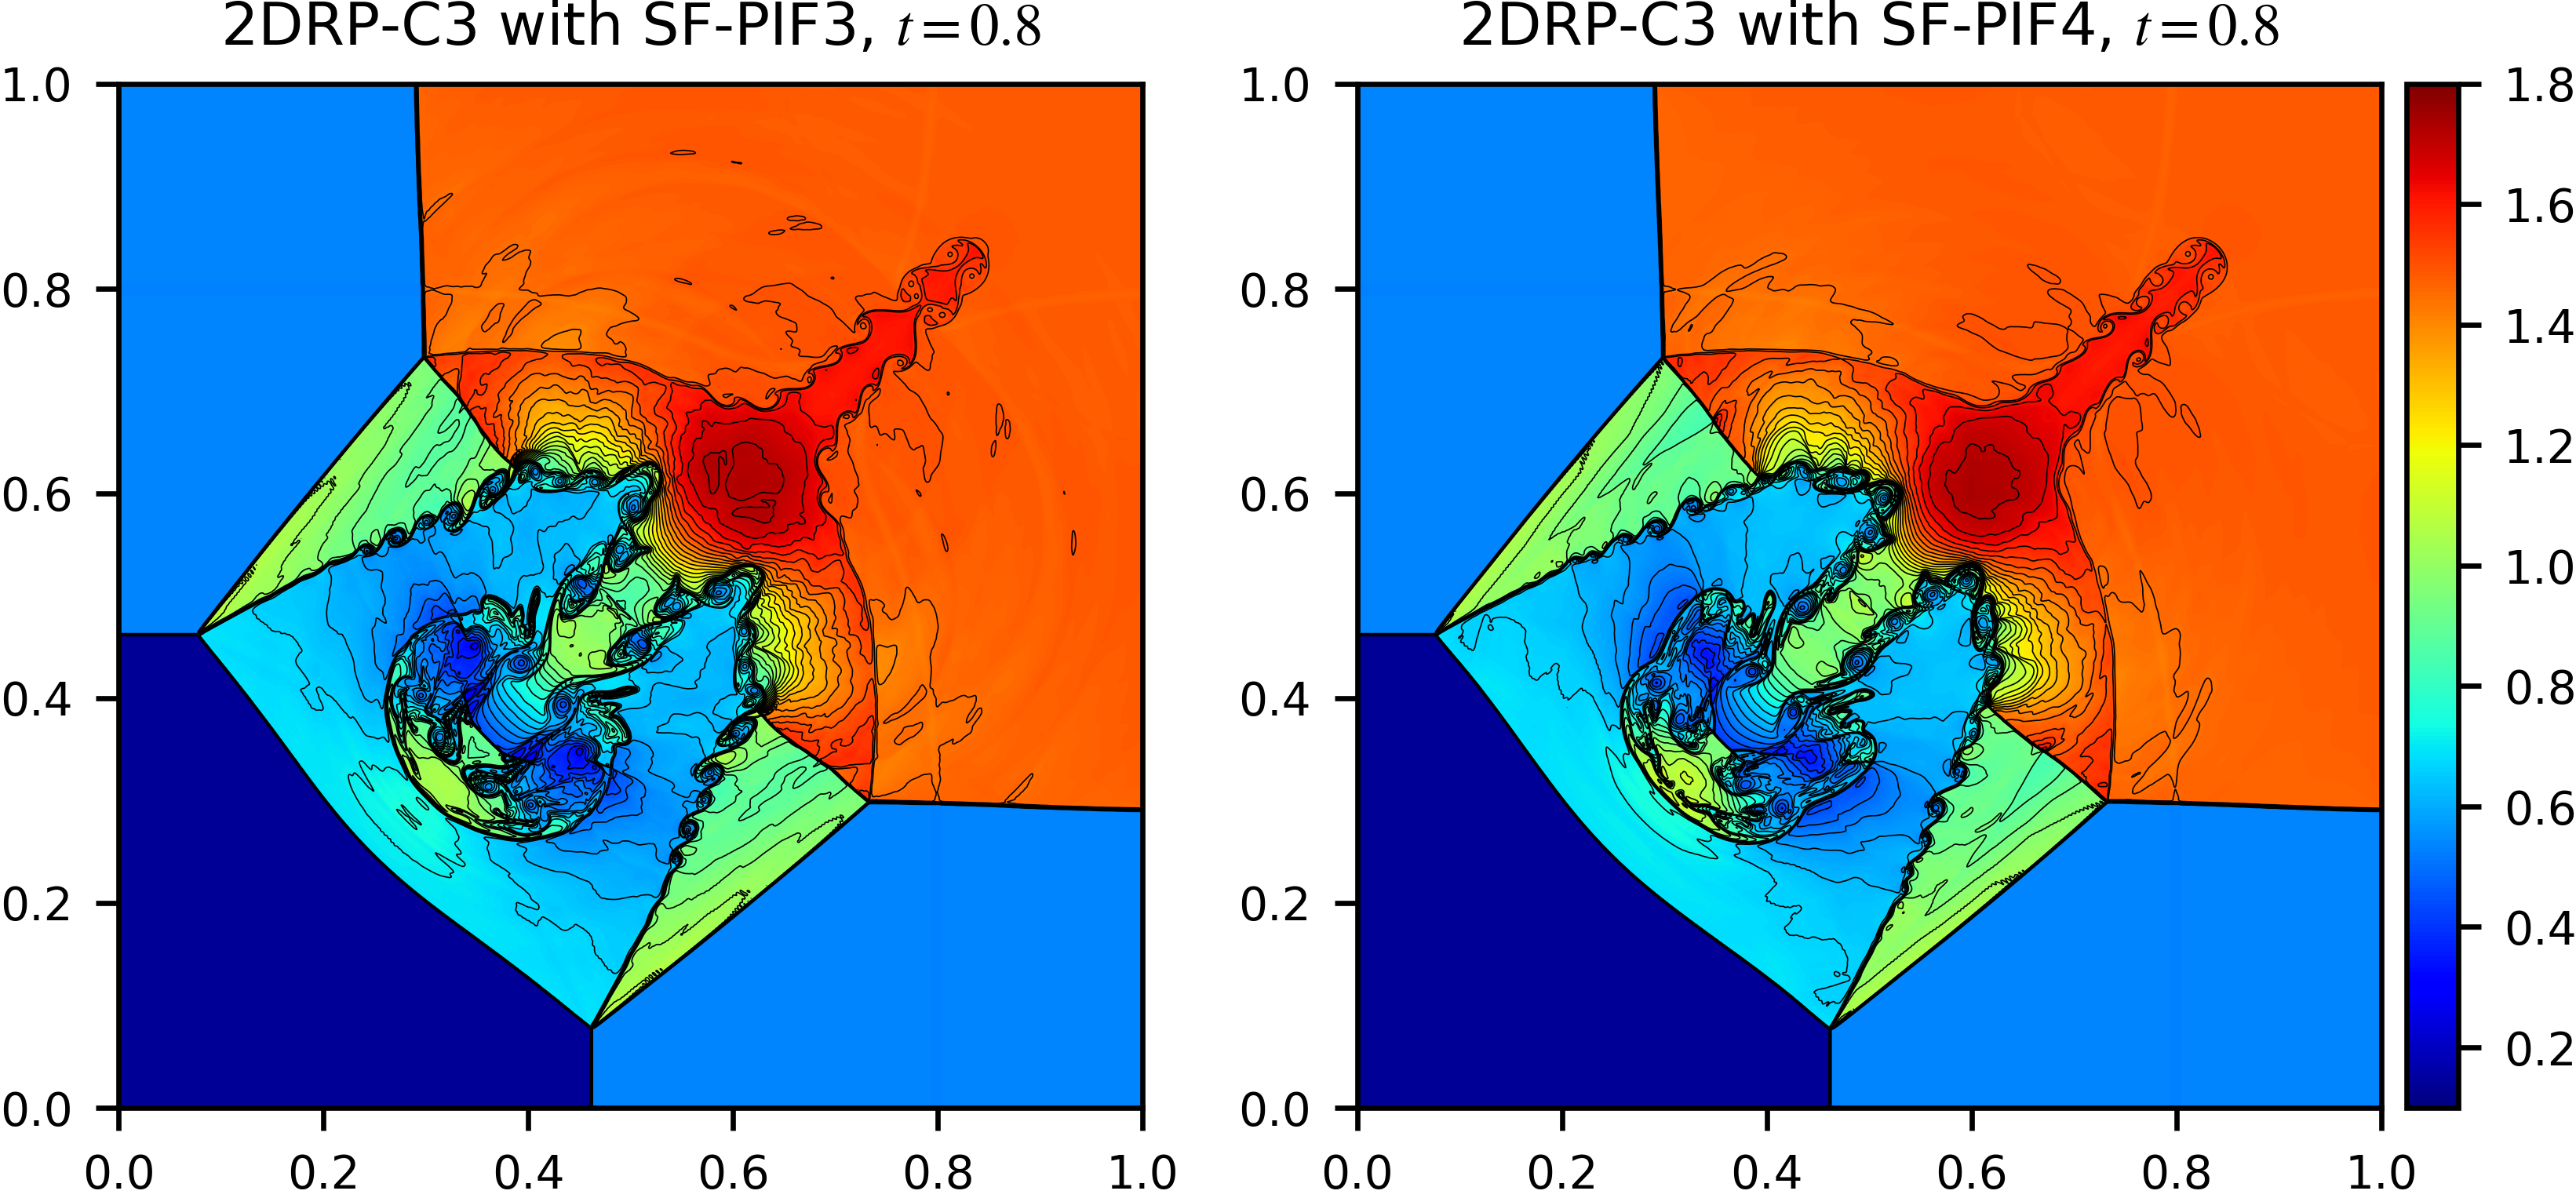
\includegraphics[width=0.9\textwidth]{fig/2drp_c3_weno5_sfPIF_1600.png}
    \end{subfigure}
    \caption{The density maps of Configuration 3 at \( t = 0.8 \).
        \textbf{Left column:} The solutions using RK3 (top) and SF-PIF3 (bottom).
        \textbf{Right column:} The solutions using RK4 (top) and SF-PIF4 (bottom).
        Forty levels of black contour lines are over-plotted in each figure
        with the same range of the color map.
        All simulations are performed on a \( 1600 \times 1600 \) grid resolution.
        }\label{fig:2drp_c3}
\end{figure}

The results at \( t = 0.8 \) are shown in~\cref{fig:2drp_c3}.
The pseudo-colors represent the density map ranging between \( [0.1, 1.8] \), and
40 contour lines within the same range are over-plotted as solid black lines.

As illustrated in the figures, all four different temporal schemes produce well-known,
acceptable results, keeping the assumed diagonal symmetry exceptionally well on this high resolution.
This problem is highly nonlinear, involving formations of the upward-moving jet,
the downward-moving mushroom-jet, secondary Kelvin-Helmholtz instabilities exhibited
as the small-scale vortical rollups along the slip lines and along the stems of the two jets.
Therefore, it is a non-trivial task to address if a method under consideration is
\textit{better} or \textit{worse} based on the number of such rollups in the simulations
without a systemic comparison analysis requiring extensive, careful validation and verification tests
that are beyond the scope of this dissertation.
At best, such quantification can only provide
proof of intrinsic information about the amount of numerical dissipation of each method.
From this perspective, one concludes that the two SF-PIF solutions produce
the equivalent amount of vortical rollups compared with the corresponding RK solutions,
although their different shapes on the downward jets,
confirming the validity of the recursive SF-PIF methods
on the presence of the shocks in 2D simulations.





\subsection{Double Mach reflection}\label{subsec:dmr_weno}

The double Mach reflection (DMR) test problem was firstly introduced by
Woodward and colella~\cite{woodward1984numerical}.
At initial, a planar shock is located at the left side of the domain
with a \( \ang{30} \) to the reflecting bottom surface.
As the shock propagates to the right, the bottom wall
continuously bounces off the shock wave and creates a round reflected shock.
The initial condition is the same as the original setup in~\cite{woodward1984numerical},
except for the doubled the \( y \)-domain size following~\cite{kemm2016proper}
to prevent numerical artifacts from the top boundary interaction with the
secondary shock wave and the slip line.

\begin{figure}
    \centering
    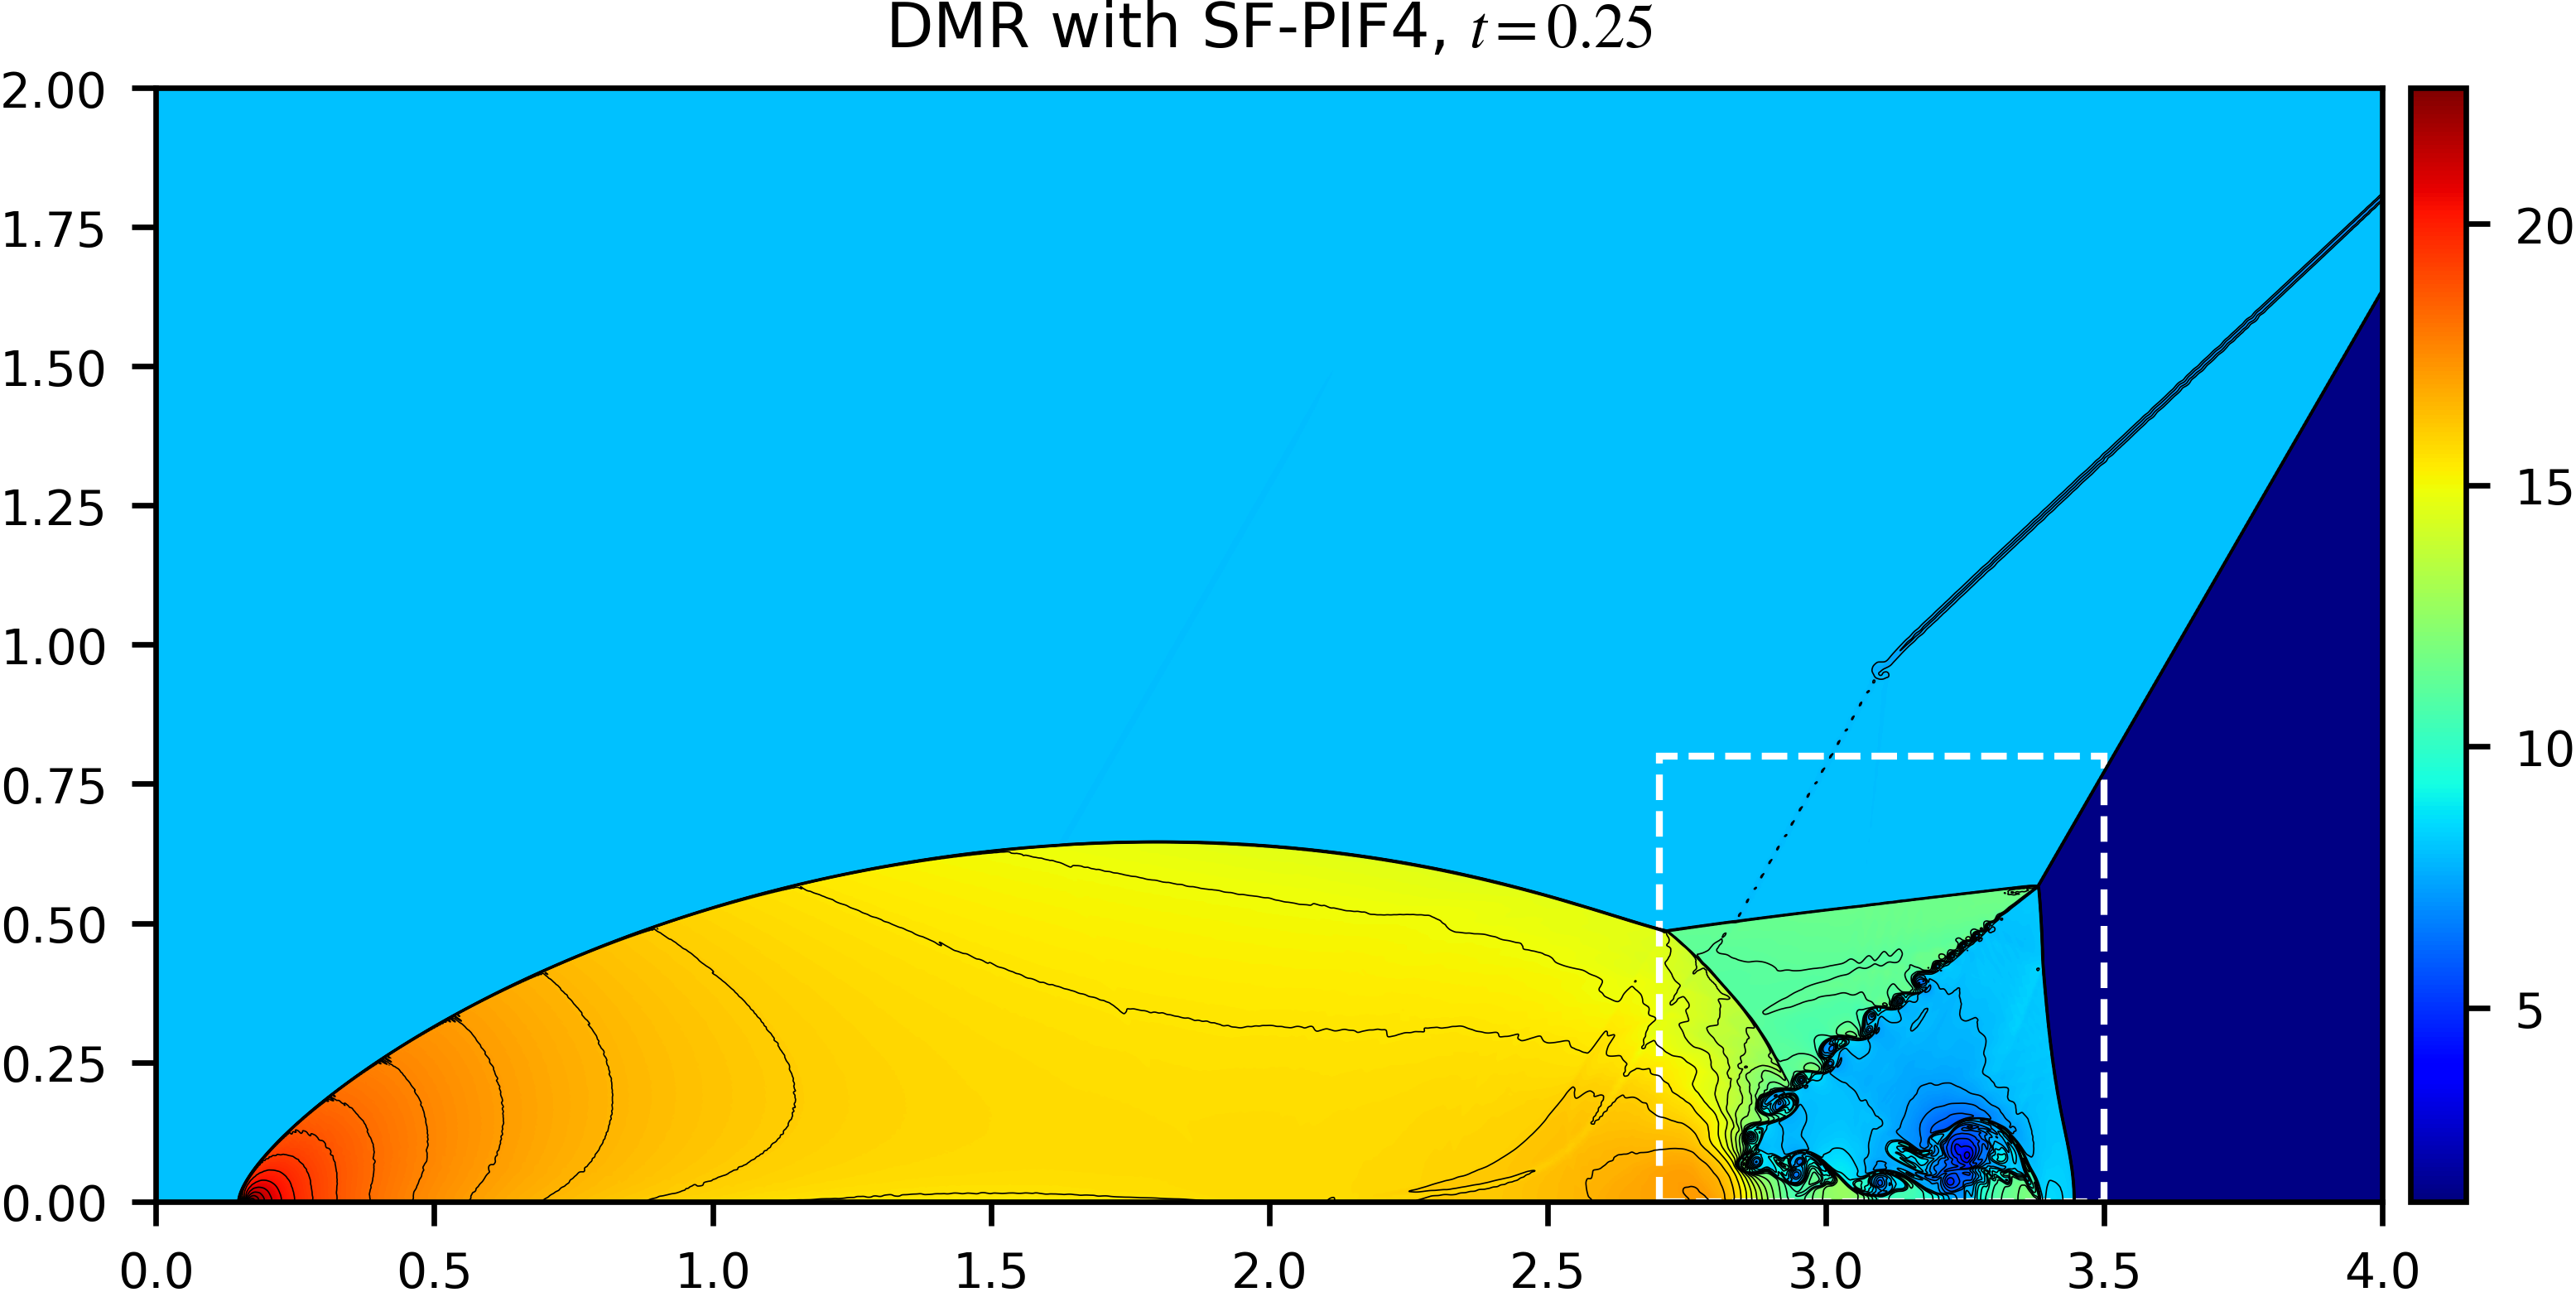
\includegraphics[width=0.85\textwidth]{fig/dmr_overview_sf4.png}
    \caption{The solution density profile of Double Mach reflection test
        solved with SF-PIF4 method on a \( 4096 \times 2048 \) grid resolution.
        The solid black curves represent the forty levels of contour lines
        ranging within the same range of the colormap.
        The white-dotted rectangle is the
        main point of interest in this simulation,
        where the jet and the primary triple point are formed.
        More detailed view of the rectangle region
        with different temporal solvers are plotted in~\cref{fig:dmr}.
    }\label{fig:dmr_overview}
\end{figure}

As the solution evolves, two contact discontinuities and two Mach stems are formed,
as well as a jet along the bottom surface. The formation of the jet is similar
to the formation of the two jets in implosion test (\cref{subsec:implosion}),
the collision of which led to the upward moving diagonal jet.
The solution density profiles resolved with the SF-PIF4 method
is portrayed in~\cref{fig:dmr_overview}.

\begin{figure}
    \centering
    \begin{subfigure}{140mm}
        \centering
        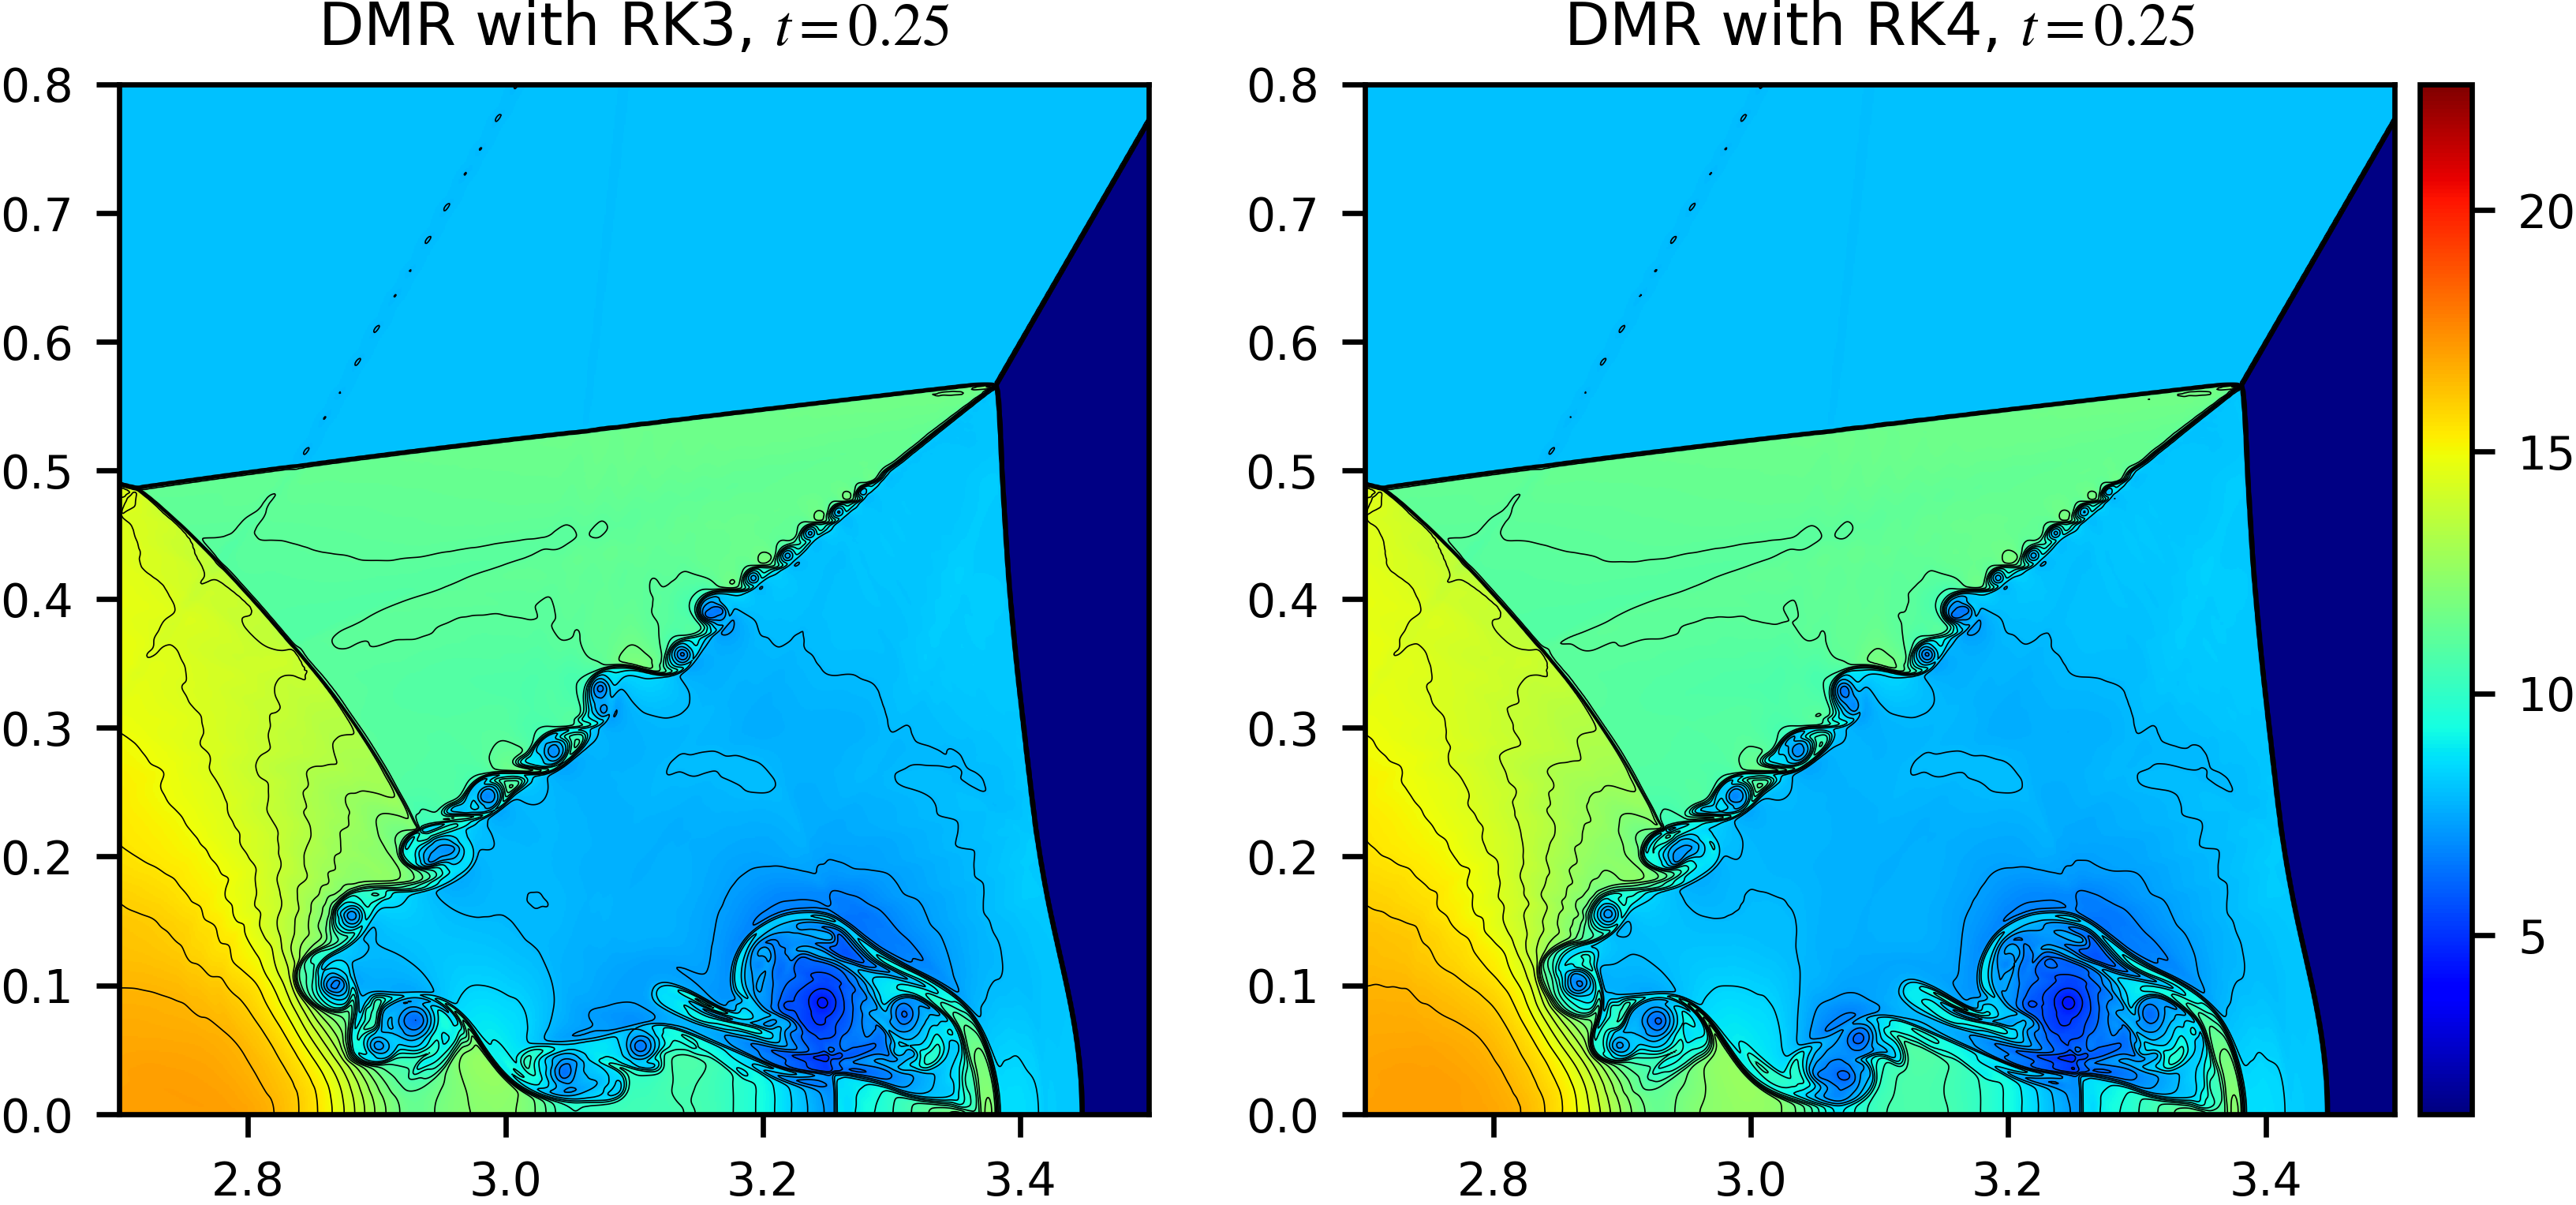
\includegraphics[width=0.95\textwidth]{fig/dmr_weno5_rk_4096y2.png}
    \end{subfigure}
    \begin{subfigure}{140mm}
        \centering
        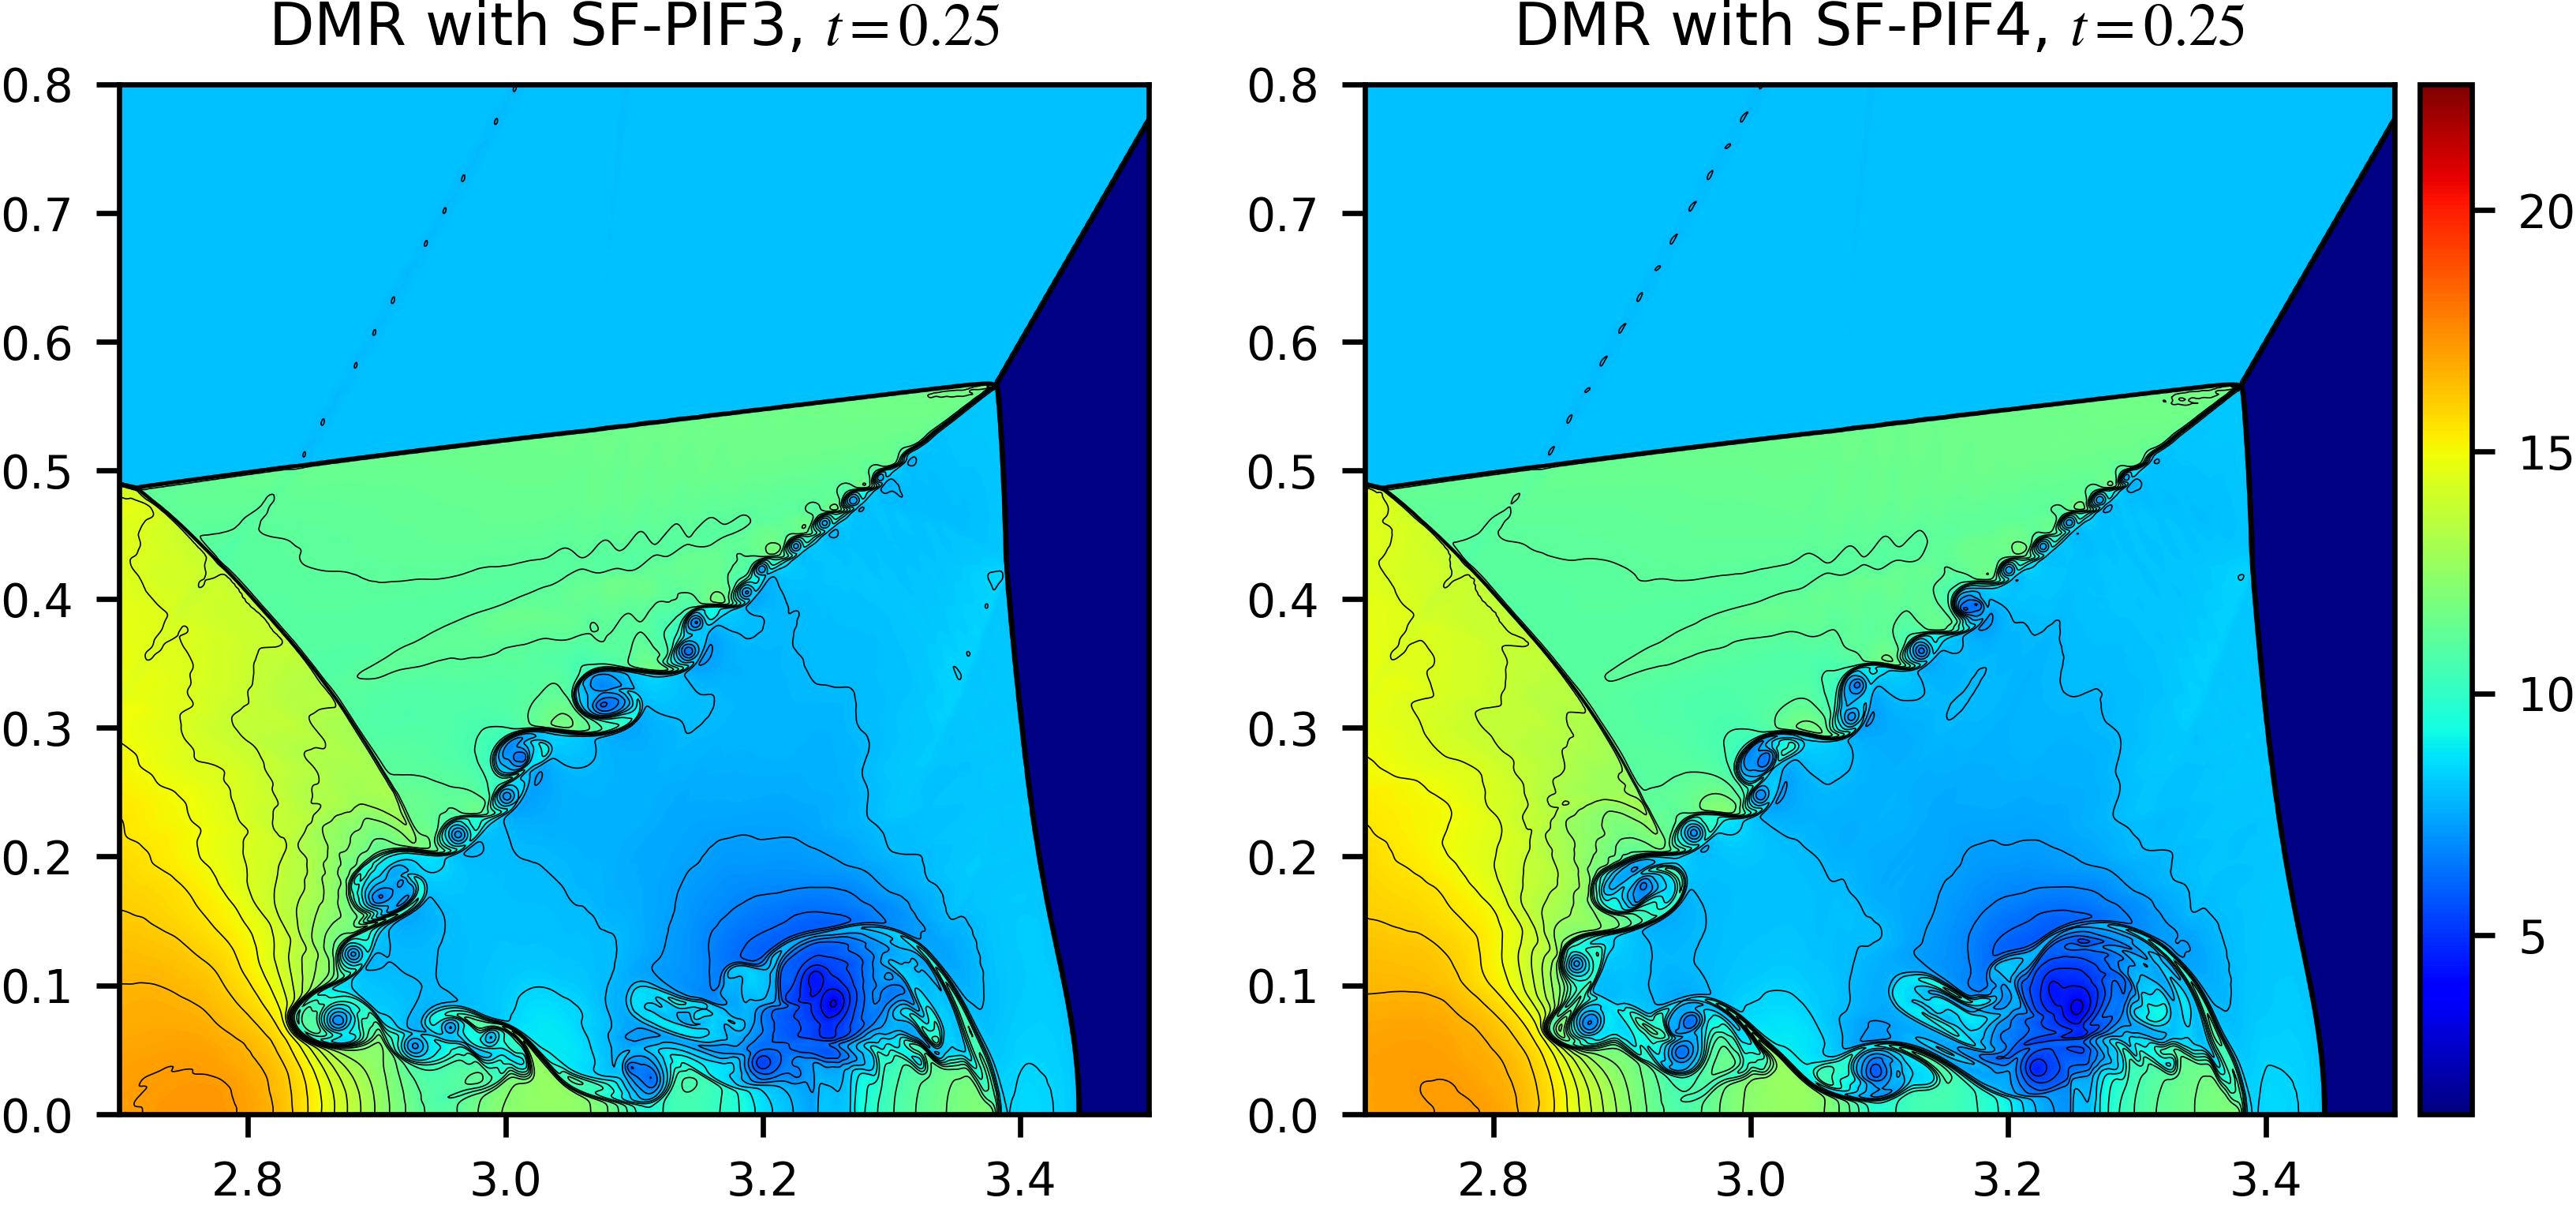
\includegraphics[width=0.95\textwidth]{fig/dmr_weno5_sf_4096y2.png}
    \end{subfigure}
    \caption{The density map of the double Mach reflection test at \( t = 0.25 \)
        zoomed-in near the jet. Forty levels of contour lines are over-plotted
        in solid black curves with the same range of the color map.
        All simulation results are performed on a
        \( 4096 \times 2048 \) grid resolution.
        \textbf{Left column:} The solutions using RK3 (top) and SF-PIF3 (bottom).
        \textbf{Right column:} The solutions using  RK4 (top) and SF-PIF4 (bottom).
    }\label{fig:dmr}
\end{figure}

\cref{fig:dmr} shows the zoomed-in views of the main point of interest in the DMR problem,
the vicinity of the jet and the primary triple point, resolved with four different temporal solvers.
Again, the results from the third- and fourth-order SF-PIF methods
produce well-acceptable results compared to the corresponding RK methods.
There are minor differences in the shape of Kelvin-Helmholtz instabilities along the
primary slip line and the bottom jet,
but the overall dynamics of the two SF-PIF solutions match well with the RK solutions,
validating the fidelity of the proposed SF-PIF methods in the presence of a strong shock.



\subsection{3D Riemann problem}\label{subsec:3drp}

The 3D Riemann problem is the 3D extension of the 2D Riemann problem described in~\cref{subsec:2drp_c3_weno},
introduced by Balsara~\cite{balsara2015three}.
Initially, each octant of the computational domain,
\( [-1, 1] \times [-1, 1] \times [-1, 1]\),
has constant initial conditions,
each of which will carry out 2D Riemann problem
including the diagonal plane of the 3D computational cubic.

\begin{figure}
    \centering
    \begin{subfigure}{140mm}
        \centering
        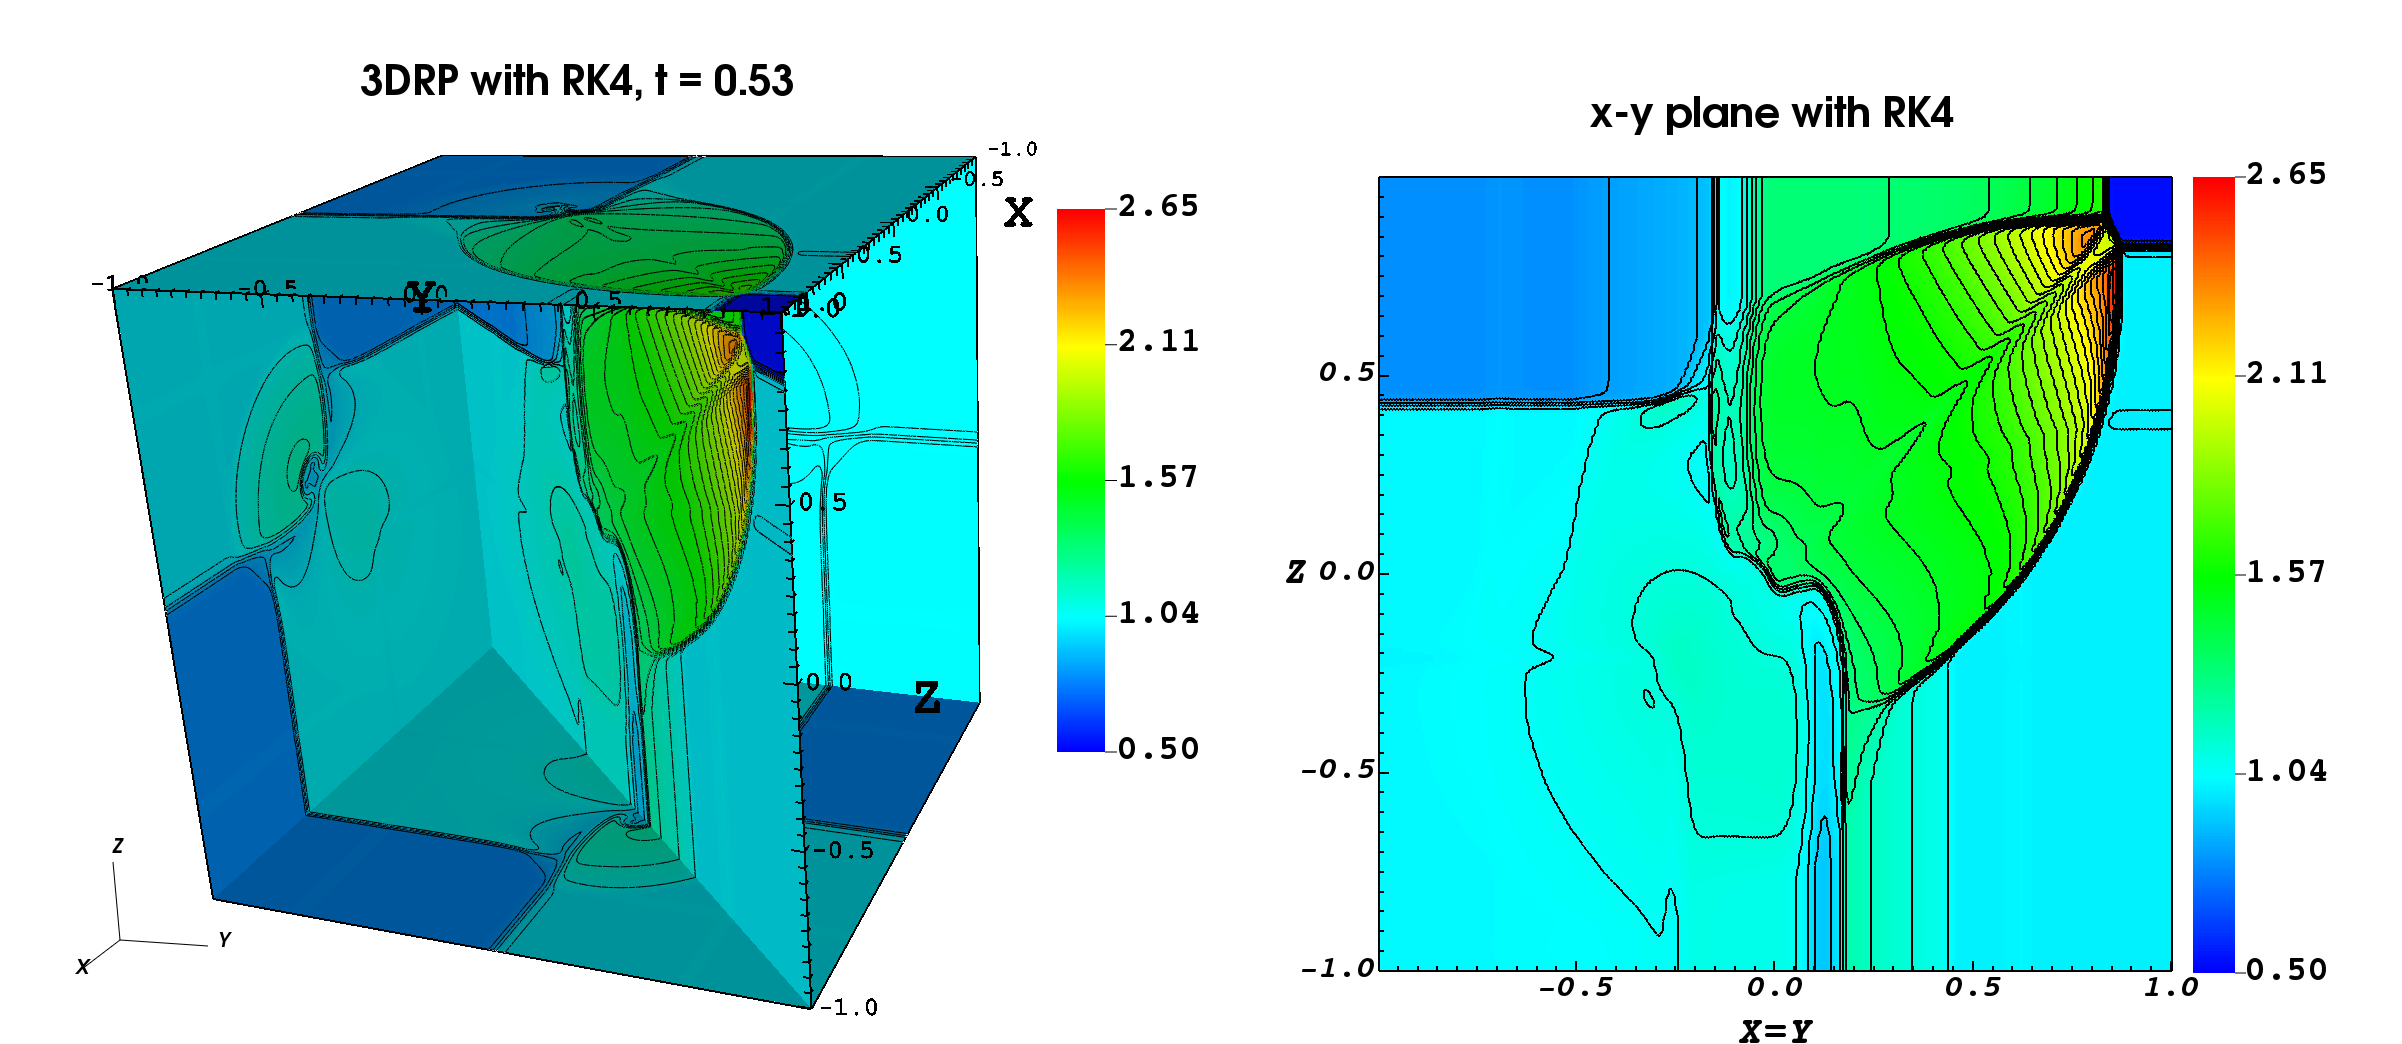
\includegraphics[width=0.95\textwidth]{fig/3drp_all_rk4.png}
    \end{subfigure}
    \begin{subfigure}{140mm}
        \centering
        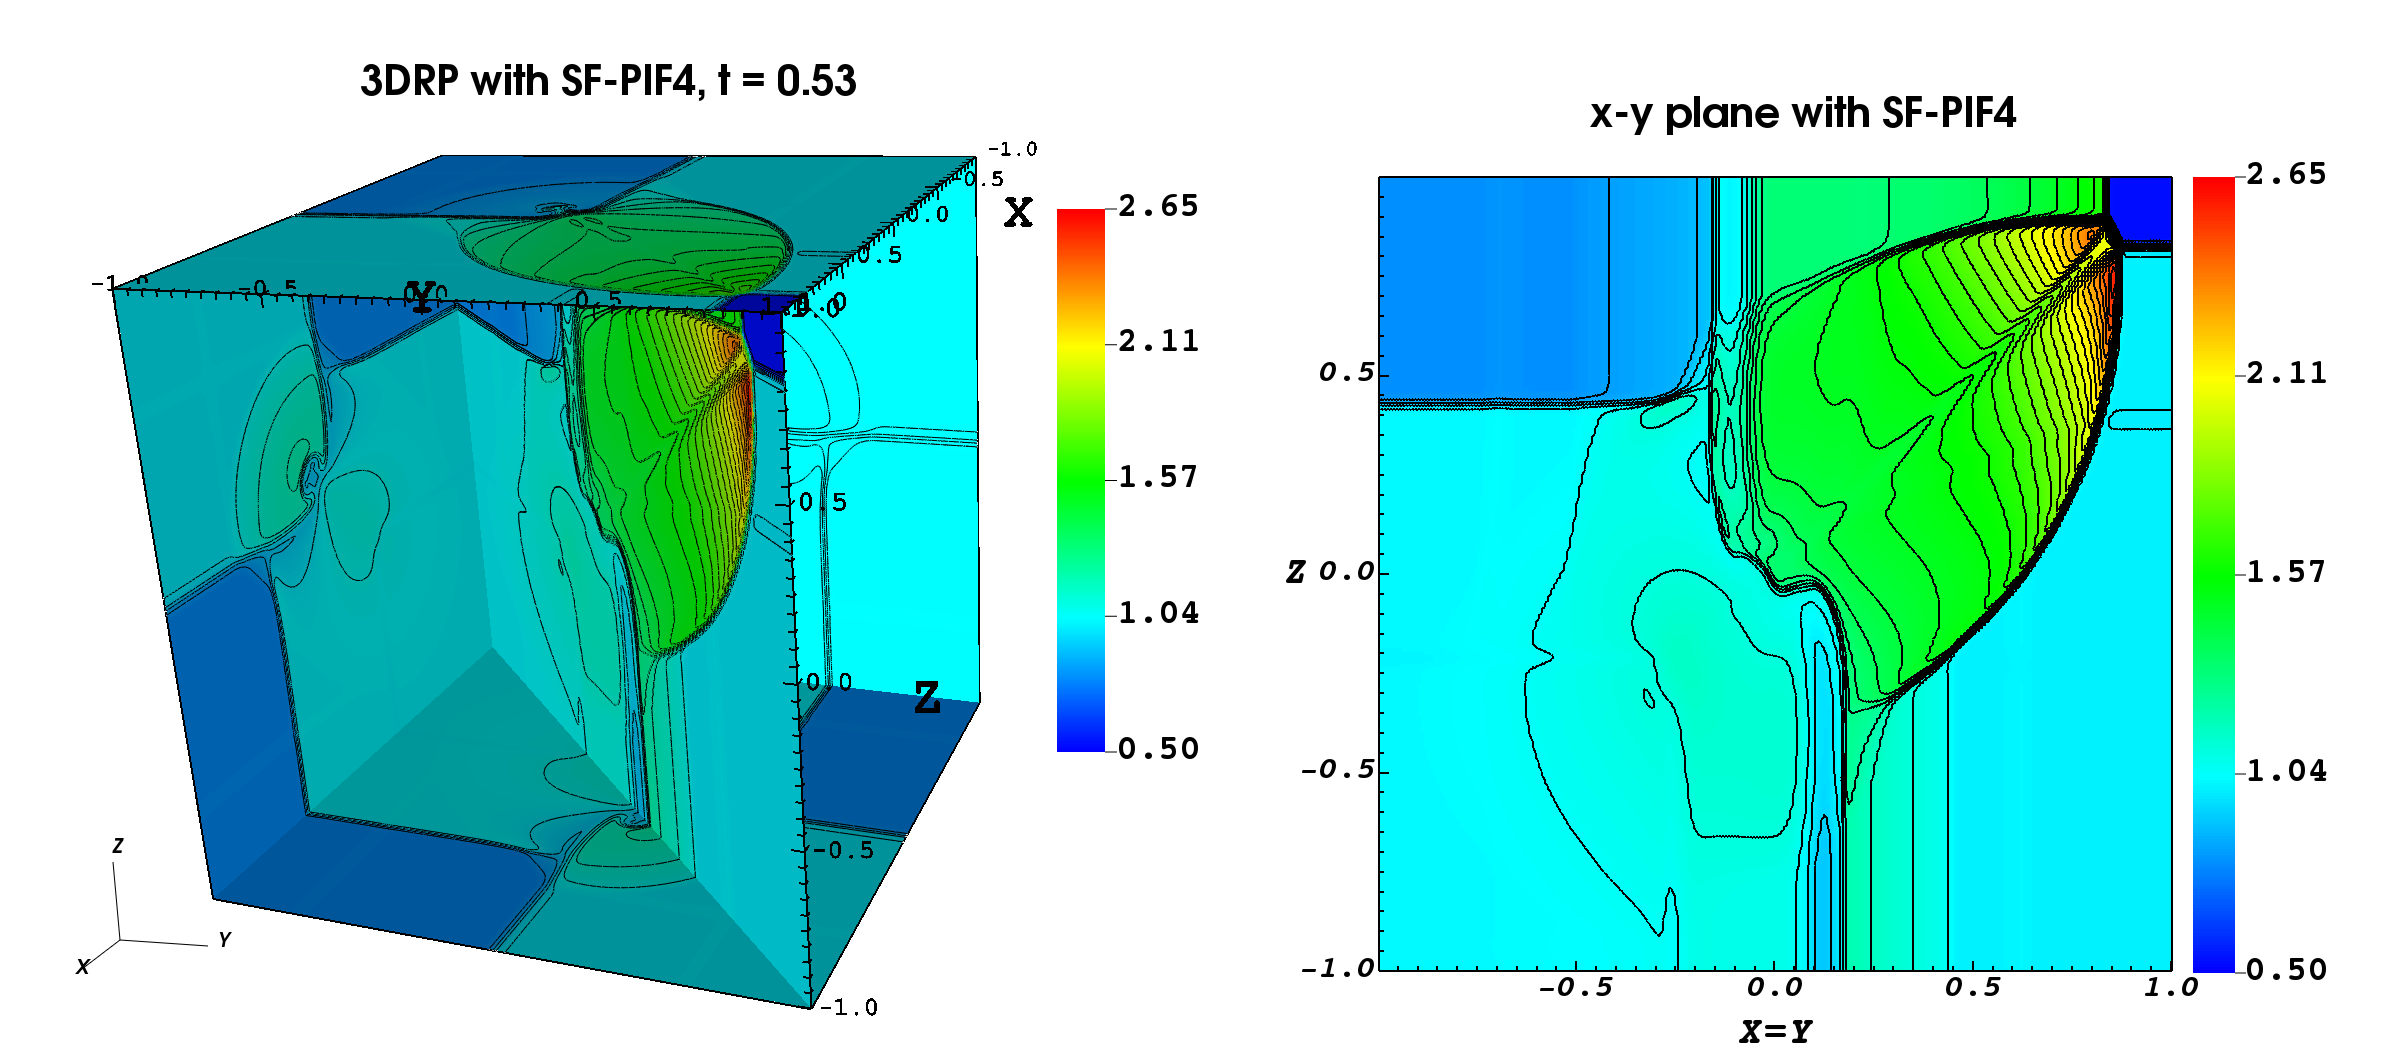
\includegraphics[width=0.95\textwidth]{fig/3drp_all_sf4.png}
    \end{subfigure}
    \caption{The density maps of the 3D Riemann problem test at \( t = 0.53 \).
        Forty contour lines are over-plotted.
        The left panels show each face's geometrical views, while 
        the right panels show
        the detailed picture of the diagonal planes.
        All simulations are performed on a \( 256 \times 256 \times 256 \) grid resolution,
        solved with RK4 (\textbf{top}) and SF-PIF4 (\textbf{bottom}) solvers.
        The Courant condition, \( C_{\text{cfl}} = 0.3 \) is used for
        calculating the timestep.
    }\label{fig:3drp}
\end{figure}

The results of 3D Riemann problem solved with RK4 and SF-PIF4 are
illustrated in~\cref{fig:3drp}. The solutions were resolved on a
\( 256 \times 256 \times 256 \) grid resolution.
The pseudo-color map ranges between \( [0.5, 2.65] \),
and 40 levels of contour lines are over-plotted using the same range.
As depicted in~\cref{fig:3drp}, each surface of 3D computational domain
evolves different 2D Riemann problems, including the diagonal plane which is
separately plotted on the left panel.
The recursive SF-PIF4 method is able to capture all the important features as much as the RK4 result,
confirming the validity of the SF-PIF4 method in 3D simulation with strong shocks.

\begin{table}
    \centering
    \caption{Performance results for the 3DRP test problem.
        All performance results (measured in seconds) are averaged over
        five simulation runs conducted on 16 nodes.% of \textit{lux} cluster.
        Each node has 2 \( \times \) 20-core Intel Xeon Gold 6248 (Cascade Lake) CPUs,
        and the simulation utilized 512 parallel threads for each run.
    }\label{table:3drp}
    \begin{adjustbox}{width=\textwidth}
        \begin{tabular}{@{}cccccccccccc@{}}
            \toprule
            \multirow{2}{*}{Grid Resolution} & \multicolumn{2}{l}{RK3} &  & \multicolumn{2}{l}{SF-PIF3}
                    & & \multicolumn{2}{l}{RK4} & & \multicolumn{2}{l}{SF-PIF4} \\
            \cmidrule(lr){2-3} \cmidrule(l){5-6} \cmidrule(l){8-9} \cmidrule(l){11-12}
            & CPU Time & Speedup &  & CPU Time & Speedup & & CPU Time & Speedup & & CPU Time & Speedup\\
            \midrule
            \( 64 \times 64 \times 64 \)   & \SI{1.79}{\second} & 1.0 &  & \SI{1.09}{\second} & 0.61 & &
                \SI{2.95}{\second} & 1.64 &  & \SI{2.67}{\second} & 1.49 \\
            \( 128 \times 128 \times 128 \) & \SI{15.62}{\second} & 1.0 &  & \SI{7.63}{\second} & 0.49 & &
                \SI{25.88}{\second} & 1.66 &  & \SI{18.97}{\second} & 1.21 \\
            \( 256 \times 256 \times 256 \) & \SI{191.00}{\second}   & 1.0 &  & \SI{82.02}{\second} & 0.43 & &
                \SI{321.34}{\second} & 1.68 &  & \SI{201.40}{\second} & 1.05 \\
            \( 512 \times 512 \times 512 \) & \SI{2679.85}{\second}  & 1.0 &  & \SI{1173.54}{\second} & 0.44 & &
                \SI{4507.88}{\second} & 1.68 &  & \SI{2817.78}{\second} & 1.05 \\
        \end{tabular}
    \end{adjustbox}
\end{table}

\cref{table:3drp} shows the performance results for the 3D Riemann problem test
on four grid resolutions.
As shown in the table, the SF-PIF4 method demonstrates nearly the same performance
as the \textit{third}-order RK method, especially in high-resolution cases.
It is important to note that the performance gains from the SF-PIF methods
are more compensated on the high-resolution grids,
which are indispensable for high fidelity physical simulation studies.

\section{SF-PIF method with GP-WENO}\label{sec:result_gpweno}

As mentioned in~\cref{chap:sfpif}, the SF-PIF method is an entirely independent temporal solver,
which does not require any modification in the spatial high-order part of the simulation codes
alike RK methods.
As the purpose of demonstrating the portability of the SF-PIF method,
this section will conduct several test problems using GP-WENO
(instead of the conventional WENO as in the previous sections) described in~\cref{subsec:gp}
as a spatial high-order reconstruction method
combining with SF-PIF methods for time integration strategy.

\subsection{Hyperparameters}\label{subsec:hyper_params_gpweno}

Unlike the polynomial-based reconstruction schemes,
the GP method lacks any analytical considerations of the behavior of numerical errors
with respect to the grid resolutions.
This is further complicated by the use of nonlinear weighting in the GP-WENO method,
which is necessary to capture the discontinuities appropriately.
Consequently, direct numerical experiments
should be conducted to predict the numerical errors from the GP-WENO method.

The GP-WENO method has two hyperparameters that need to be tuned,
the length hyperparameter \( \ell \)
and the shock-capturing hyperparameter \( \sigma \).
The numerical errors from the 2D vortex advection problem
with varying hyperparameters are illustrated in~\cref{fig:gp_hp_cmap}.
The simulations are conducted on \( 400 \times 400 \) grid resolutions,
resolved with SF-PIF3 temporal solver
with the same setup in~\cref{subsec:vortex_weno}.
As dotted white lines represent,
the minimum error has been found with \( \ell = \sigma = 1\)
for this systematic test.

\begin{figure}
    \centering
    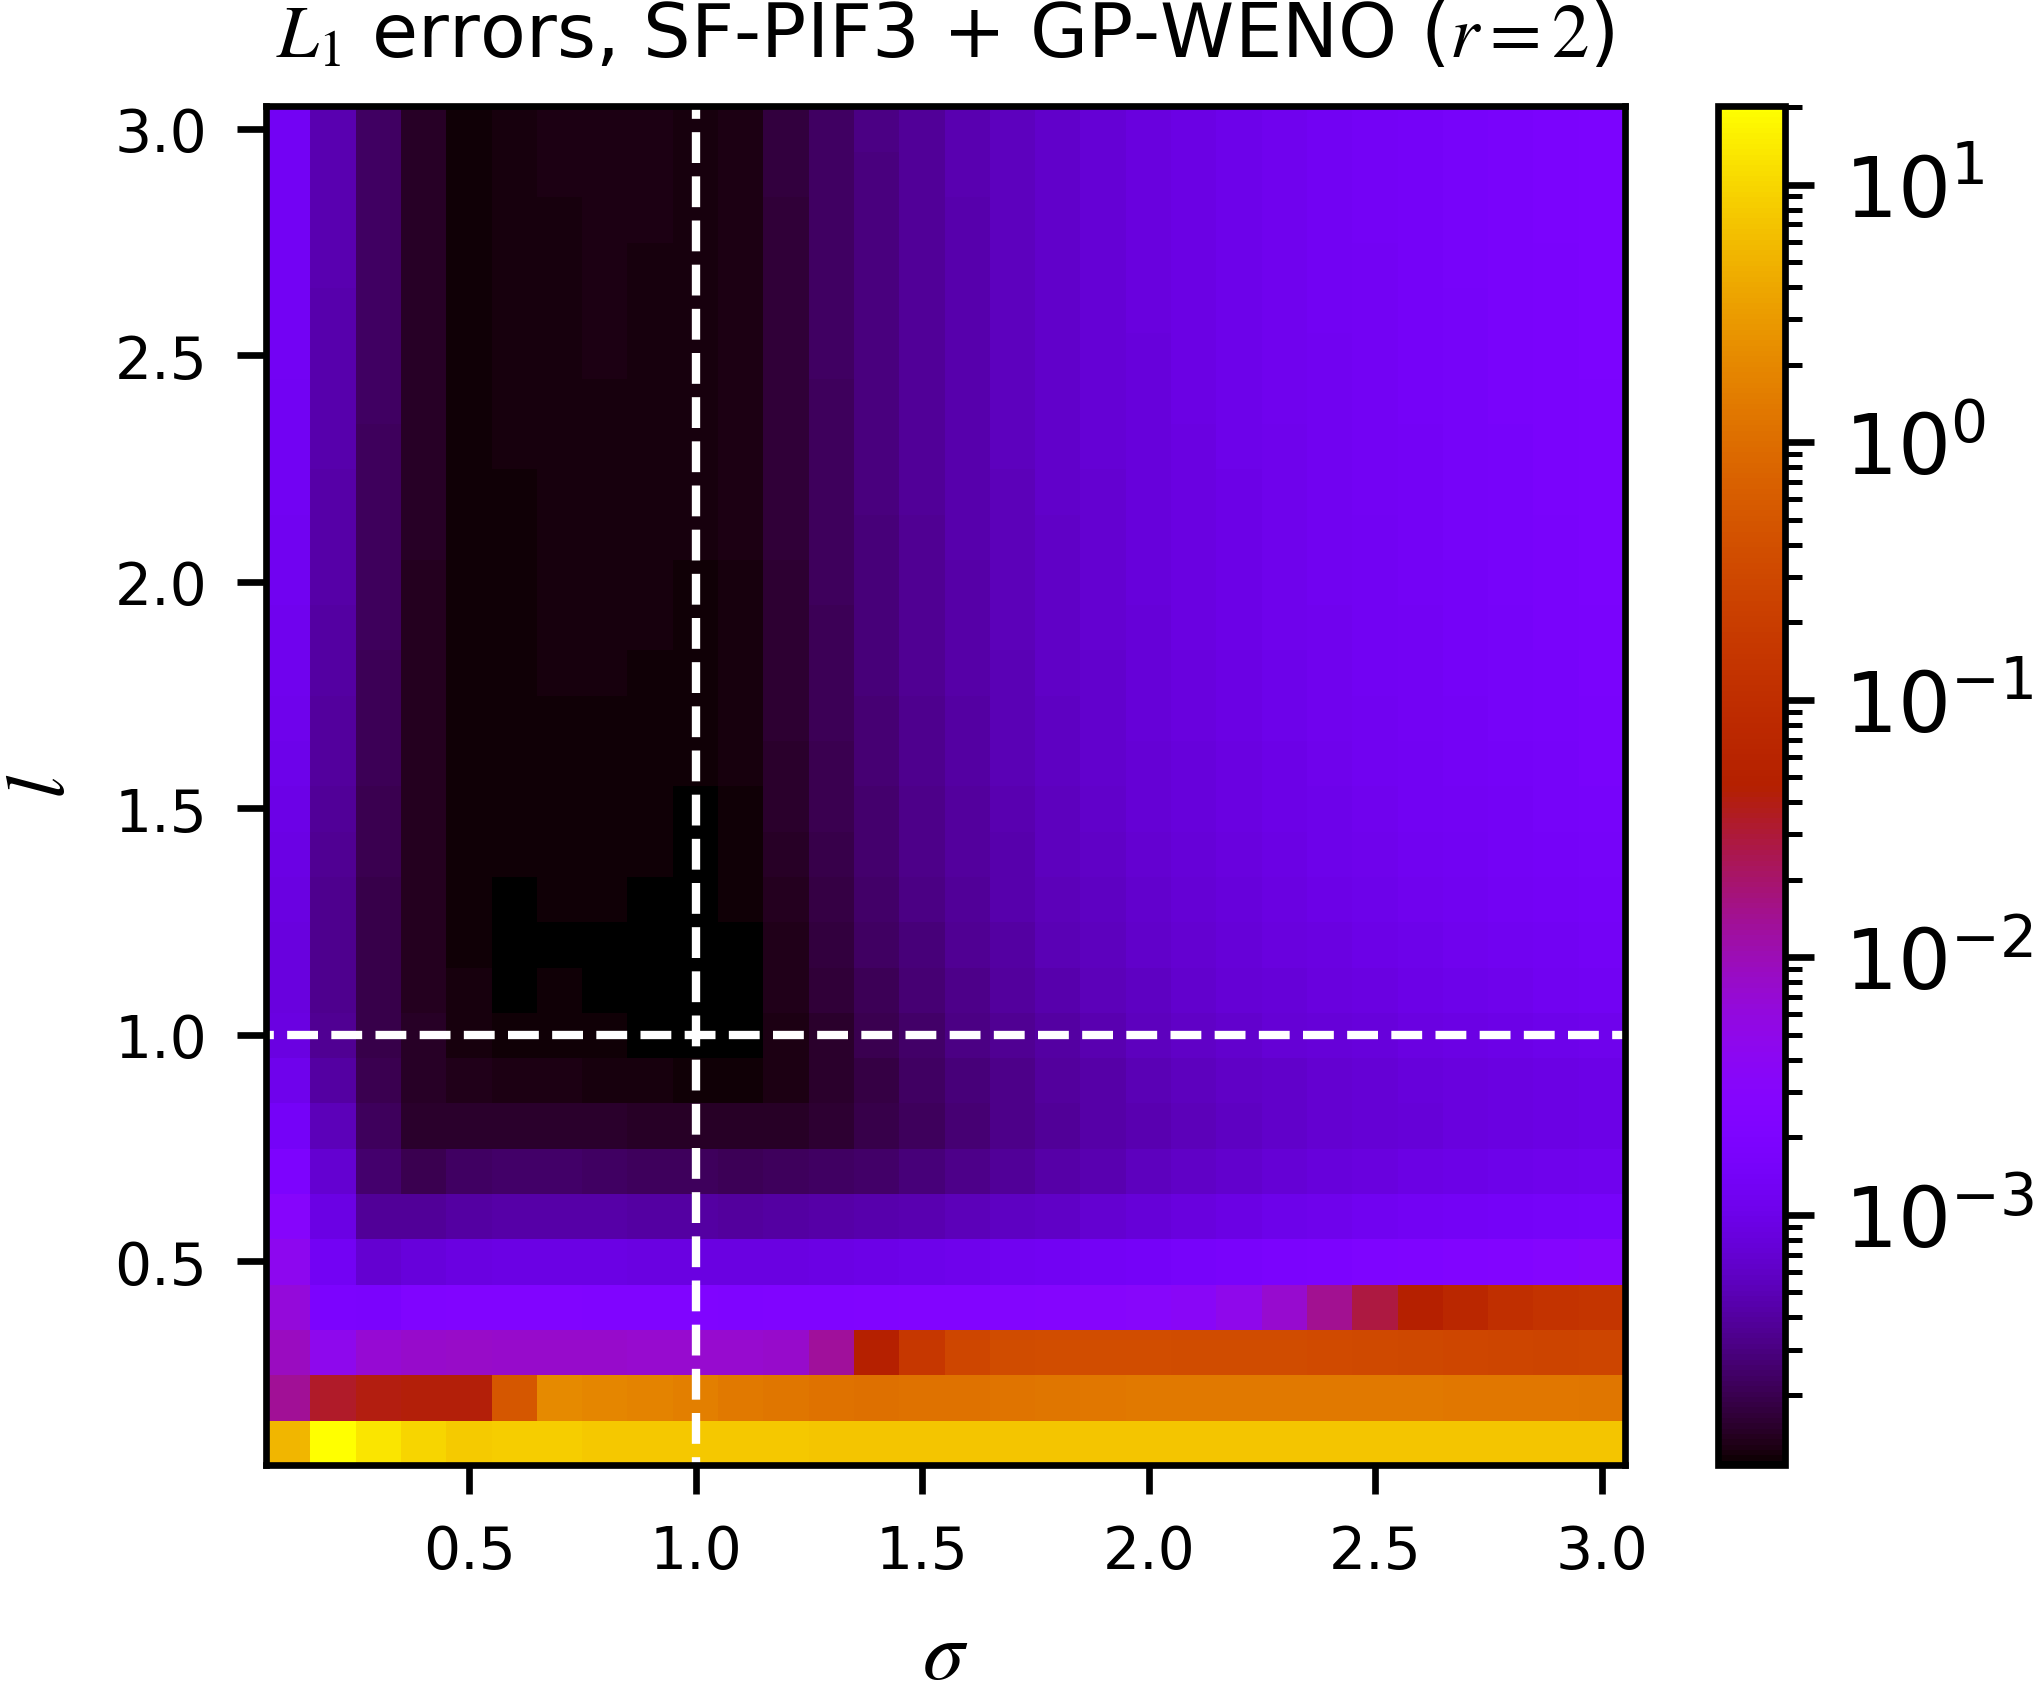
\includegraphics[width=0.85\textwidth]{fig/hp_cmap_gp2_sf3.png}
    \caption{The \( L_{1} \) errors of vortex advection problem solved by
        GP-WENO and SF-PIF3 on a \( 400 \times 400 \) grid resolution.
        The radius of GP-WENO stencil is \( r=2 \), which is the same
        stencil size of the fifth-order WENO method.
        Using other temporal solvers produces the same pattern,
        and omitted in this study.
        The white dotted-lines are represent the
        hyperparameters of minimum error.
    }\label{fig:gp_hp_cmap}
\end{figure}

\begin{figure}
    \centering
    \begin{subfigure}{70mm}
        \centering
        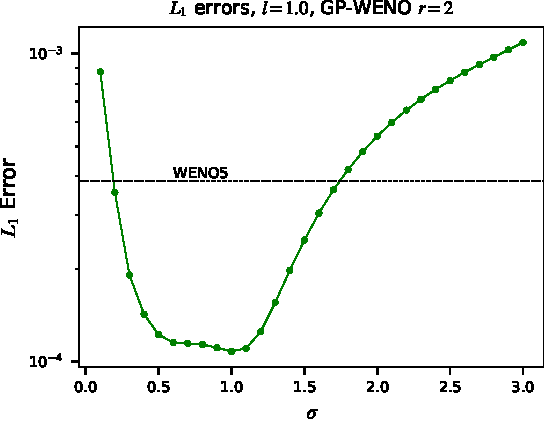
\includegraphics[width=0.95\textwidth]{fig/hp_best_ell_gp2_sf3}
    \end{subfigure}
    \begin{subfigure}{70mm}
        \centering
        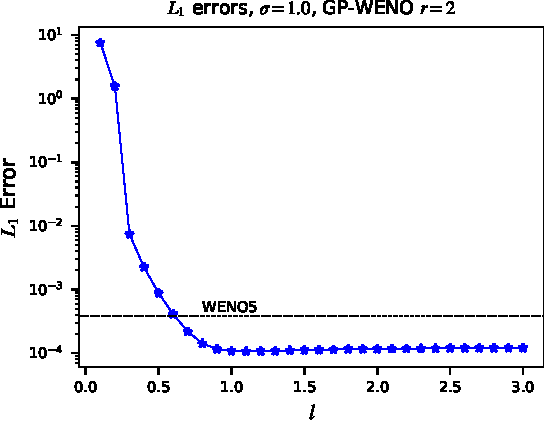
\includegraphics[width=0.95\textwidth]{fig/hp_best_sig_gp2_sf3}
    \end{subfigure}
    \caption{The slices of~\cref{fig:gp_hp_cmap} at the minimum error.
        The horizontal dotted line is the target error obtained from WENO method
        with same configurations.
    }\label{fig:gp_hp_best}
\end{figure}

\cref{fig:gp_hp_best} shows the slice plots by following the dotted lines
in~\cref{fig:gp_hp_cmap}, showing the \( L_{1} \) errors
with the best choice of \( \ell \) and \( \sigma \).
Surprisingly, the shock-capturing hyperparameter \( \sigma \) affects the solution accuracy,
even though the solution is entirely smooth.
Theoretically speaking, the vortex advection test is a nonlinear smooth problem,
and \( \sigma \) only plays a role in the presence of a shock discontinuity;
thus, it has to have the same errors across all sigma values.
The different errors with varying sigma in the smooth problem are the indication
of numerical errors in calculating nonlinear weights of GP-WENO\@.
This could be arisen from calculating the linear weights,
(i.e., solving the overdetermined system~\cref{eq:gp_weno_overdetermined_matrix})
or calculating smoothness indicators in~\cref{eq:gp_smoothness_ind},
which requires further studies.
Nonetheless, since the numerical solvers are involved in calculating
both the linear weights and smoothness indicators,
e.g., the least square method and QR algorithm,
numerical errors are inevitable in GP-WENO nonlinear weights.

Notwithstanding the fact that the GP-WENO method with \( \sigma = 1 \)
has the smallest amount of \( L_{1} \) errors
from the previous tests, however,
another numerical tests argue that the large \( \sigma \) values
degrade the solution accuracy in high-resolution simulation.

\begin{figure}
    \centering
    \begin{subfigure}{70mm}
        \centering
        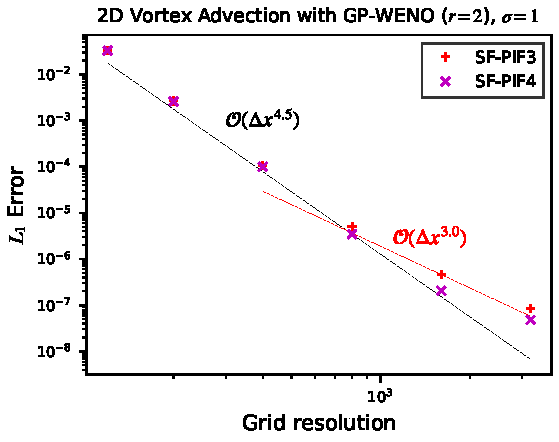
\includegraphics[width=0.95\textwidth]{fig/gp2_vortex_error_sigma1}
    \end{subfigure}
    \begin{subfigure}{70mm}
        \centering
        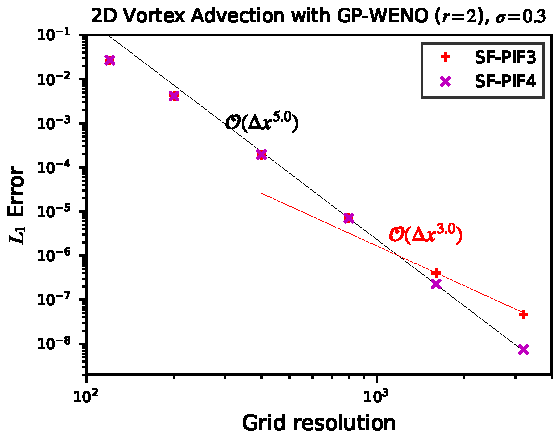
\includegraphics[width=0.95\textwidth]{fig/gp2_vortex_error_sigma03}
    \end{subfigure}
    \caption{The convergence rate of GP-WENO method with \( r=2 \) obtained by solving
        2D isentropic vortex advection problem on varying grid resolutions.
        Two temporal methods, SF-PIF3 and SF-PIF4 are used for integrating the solution,
        and the behavior of third-order and fourth-order temporal schemes
        is identical to the results from~\cref{subsec:vortex_weno}.
        The GP length hyperparameters, \( \ell = 1 \) is used for both tests,
        and the shock-capturing hyperparameter
        \textbf{Left:} \( \sigma = 1 \), and \textbf{Right:} \( \sigma = 0.3 \)
        are used.
        The tests with \( \sigma = 1 \) on the left panel have smaller absolute \( L_{1} \) error,
        but failed to maintaining the convergence rate on high-resolution grids.
        On the other hand, tests with \( \sigma = 0.3 \) demonstrate consistent
        convergence rate on all grid configurations.
    }\label{fig:gp_vortex_convergence}
\end{figure}

\cref{fig:gp_vortex_convergence} shows that the GP-WENO method's hyperparameter \( \sigma \)
affects the convergence rate significantly.
As shown in the left panel of~\cref{fig:gp_vortex_convergence},
the GP-WENO method with the choice of \( \sigma = 1 \) can not retain
the expected order of convergence rate
in high-resolution regimes
both with SF-PIF3 and SF-PIF4 methods.
On the other hand, the choice of \( \sigma = 0.3 \) on the right panel of~\cref{fig:gp_vortex_convergence}
shows similar performance results as in the discussions of~\cref{subsec:vortex_weno},
although the absolute magnitudes of \( L_{1} \) errors are slightly larger than
the case of \( \sigma = 1 \).

\begin{table}
    \centering
    \caption{The \( L_{1} \) errors, the rates of convergence,
        and the computation times for the vortex advection test
        solved using GP-WENO method with radius of \( r = 2 \).
        The hyperparameters, \( \ell = 1 \) and \( \sigma = 0.3 \)
        are used for all simulation based on the results of~\cref{fig:gp_vortex_convergence}.
        The ``Speedup'' columns represent the relative speed-ups
        compared to the WENO5 method with corresponding temporal solveers.
        All simulation runs are
        performed on the four 20-cores
        Cascade Lake Intel Xeon processors, utilized 64 parallel threads.
        CPU times are measured in seconds, averaged over 10 individual runs.
    }\label{table:vortex_gp2}
    \begin{adjustbox}{width=\textwidth}
        \begin{tabular}{@{}ccccclcccc@{}}
            \toprule
            \multirow{2}{*}{\( N_{x} = N_{y} \)} & \multicolumn{4}{c}{GP-WENO + SF-PIF3} &  & \multicolumn{4}{c}{GP-WENO + SF-PIF4} \\
            \cmidrule(lr){2-5} \cmidrule(l){7-10}
            & \(L_{1}\) error & \(L_{1}\) order & CPU Time & Speedup &  &
            \(L_{1}\) error & \(L_{1}\) order & CPU Time & Speedup \\ \midrule
            120  & \num{2.68E-2} & \--- & \SI{0.67}{\second}      & 0.95 &  & \num{2.67E-2} & \--- & \SI{1.36}{\second}     & 0.92 \\
            200  & \num{4.16E-3} & 3.65 & \SI{2.43}{\second}      & 0.88 &  & \num{4.17E-3} & 3.66 & \SI{4.97}{\second}     & 0.93 \\
            400  & \num{1.91E-4} & 4.44 & \SI{16.86}{\second}     & 0.85 &  & \num{1.94E-4} & 4.42 & \SI{33.39}{\second}    & 0.93 \\
            800  & \num{7.12E-5} & 4.75 & \SI{133.79}{\second}    & 0.87 &  & \num{7.07E-6} & 4.78 & \SI{252.08}{\second}   & 0.93 \\
            1600 & \num{4.05E-7} & 4.14 & \SI{1061.26}{\second}   & 0.88 &  & \num{2.28E-7} & 4.95 & \SI{1944.68}{\second}  & 0.93 \\
            3200 & \num{4.71E-8} & 3.10 & \SI{8375.05}{\second}   & 0.89 &  & \num{7.48E-9} & 4.93 & \SI{15514.25}{\second} & 0.95 \\
        \end{tabular}
    \end{adjustbox}
\end{table}

The detailed numerics of the GP-WENO's convergence tests are summarized in~\cref{table:vortex_gp2}.
The all simulation runs are performed with the same configurations of WENO5 tests in~\cref{table:vortex_weno_fourth};
thus, the ``Speedup'' columns portray the relative speed-ups of GP-WENO method
compared to the conventional fifth-order WENO method.
The GP-WENO method with appropriately selected hyperparameters
produces less \( L_{1} \) errors and better convergence rate
with the high-order temporal method, SF-PIF4.
On the other hand, the GP-WENO method coupled with the relatively low-order temporal solver, SF-PIF3,
experiences the convergence rate degradation more faster than the WENO5.







\subsection{Strong shock vortex interaction}\label{subsec:shock_vortex}

In order to test GP-WENO's numerical capability to capturing
a complex flow patterns with both smooth regions and discontinuous shock waves,
the strong shock vortex interaction test~\cite{cheng2019two,galbraith5th} is considered.
Initially, a Mach 1.5 stationary shock is present at \( x = 0.5 \),
and the vortex is located at the center of \( (x_{c}, y_{c}) = (0.25, 0.5) \).
As the simulation evolves, the vortex moves with the background flow,
which is traveling toward to a stationary shock.
Consequently, the vortex penetrates the stationary shock,
evolving complex fluid structures of the ``squeezed'' vortex.
The computational domain is a 2D rectangle box of \( [0,2]\times[0,1] \)
with an inflow boundary on the left and an outflow boundary on the right.
Bottom and top boundaries are reflected walls.

\begin{figure}
    \centering
    \begin{subfigure}{120mm}
        \centering
        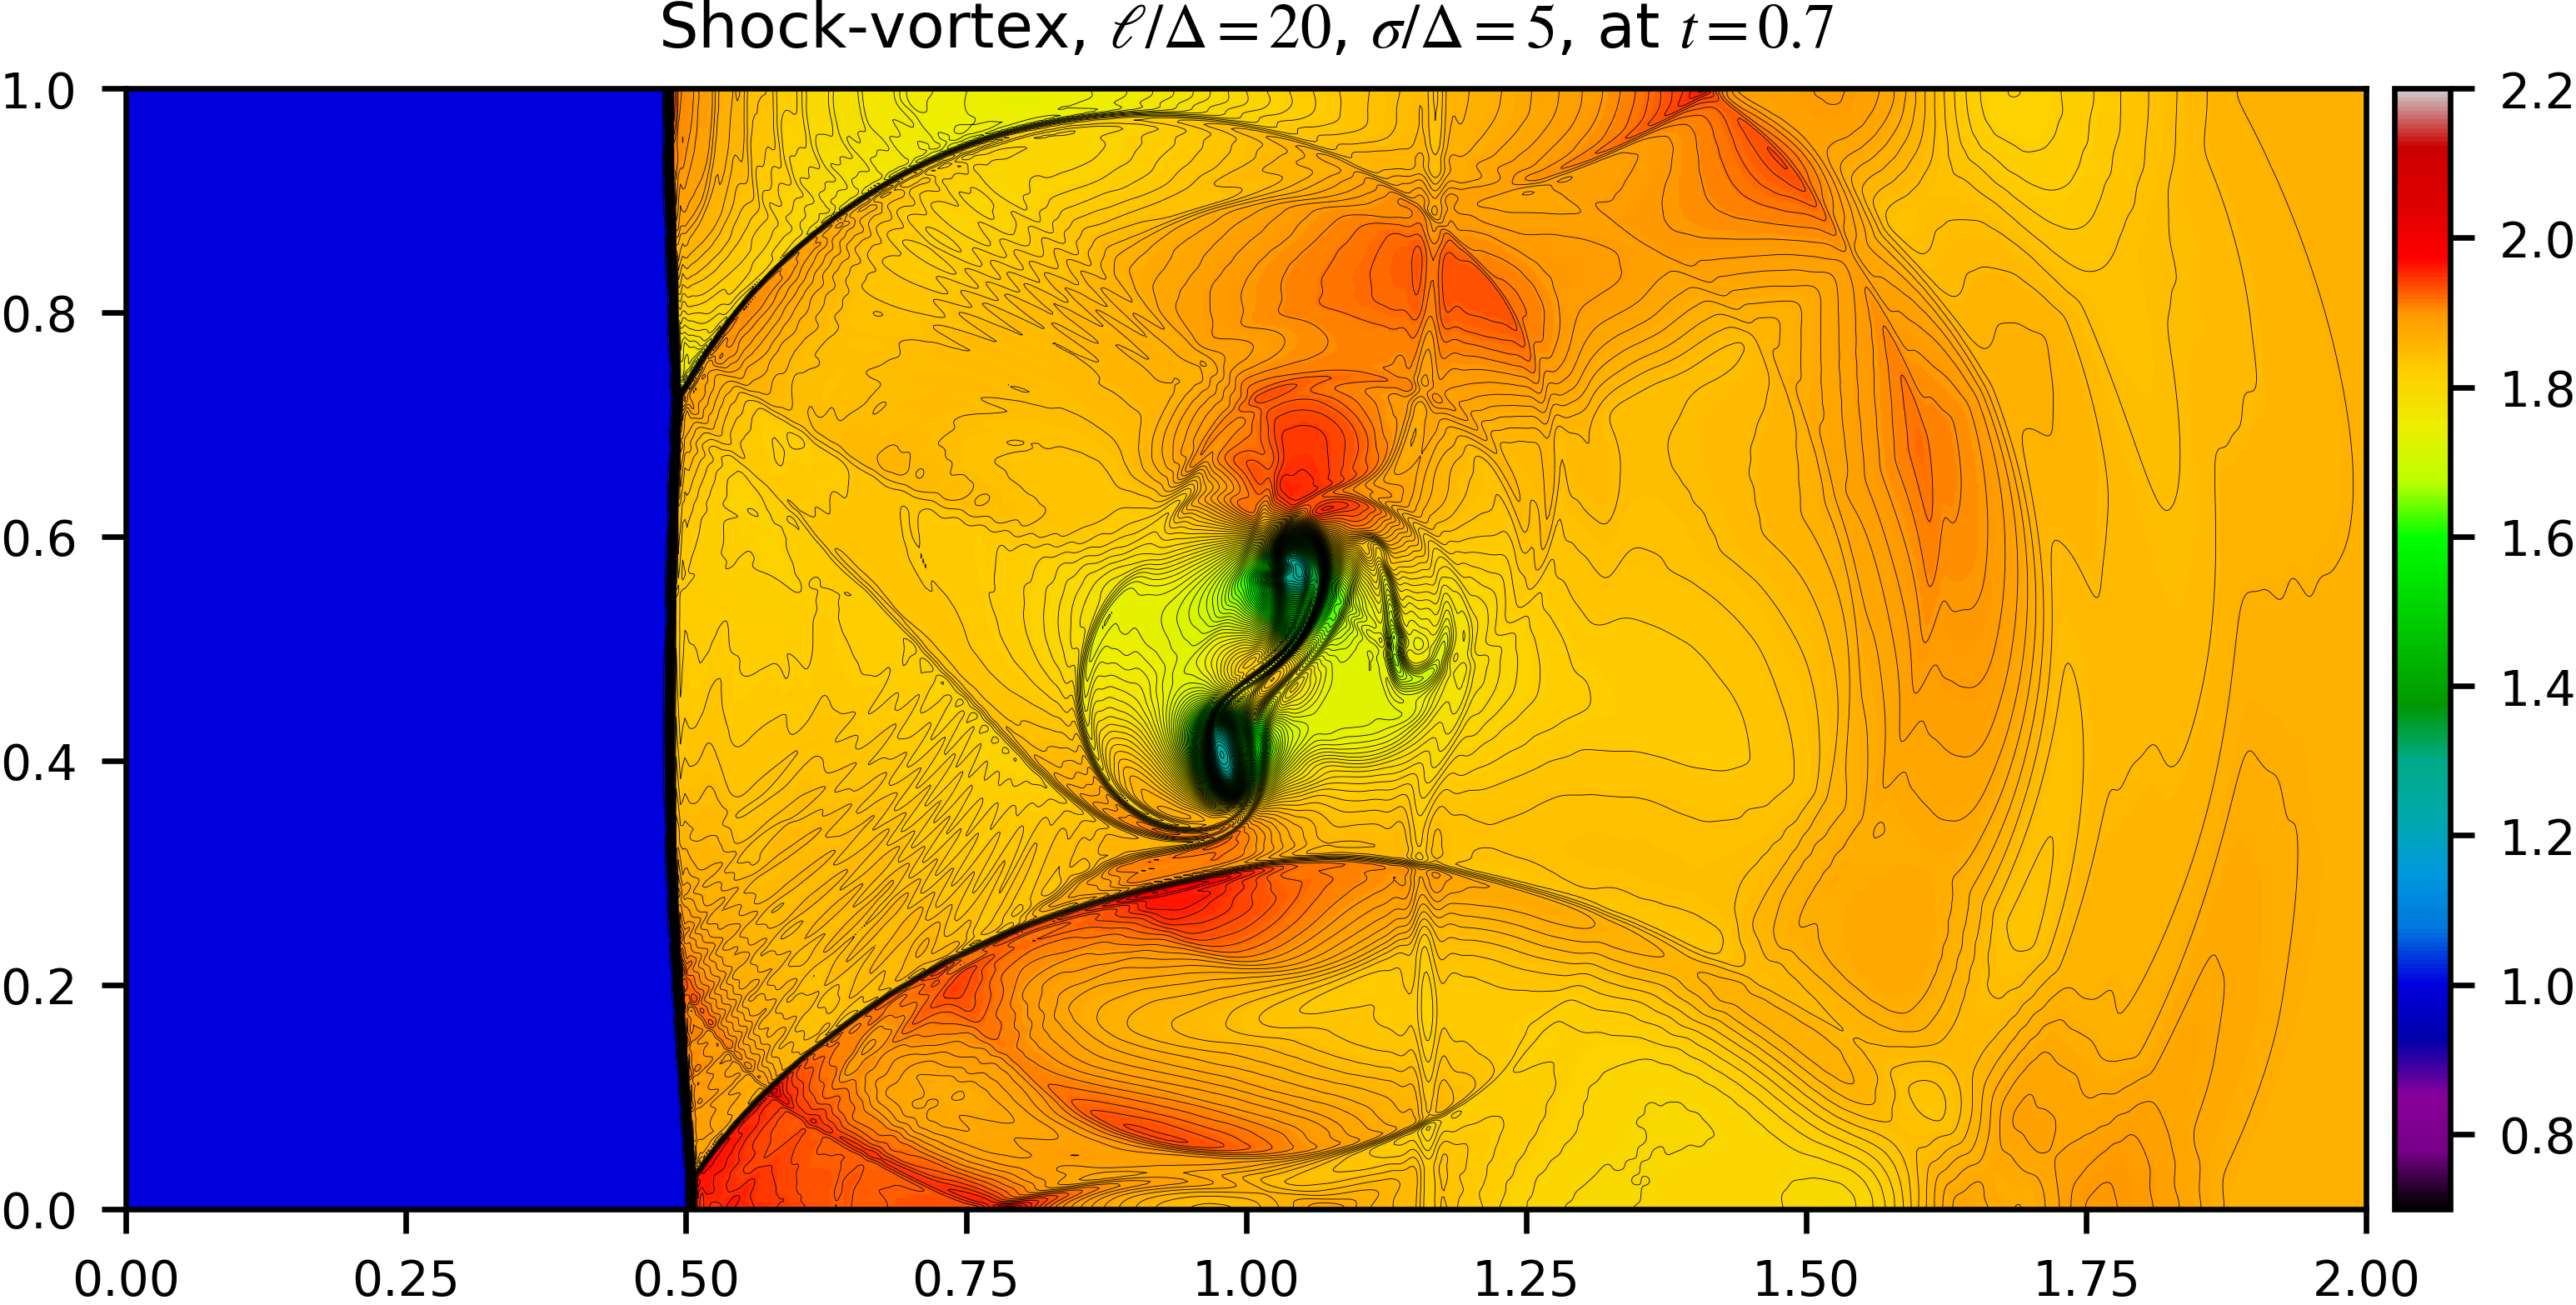
\includegraphics[width=0.95\textwidth]{fig/shockvortex_gp_ed20_sd5.png}
    \end{subfigure}
    \begin{subfigure}{120mm}
        \centering
        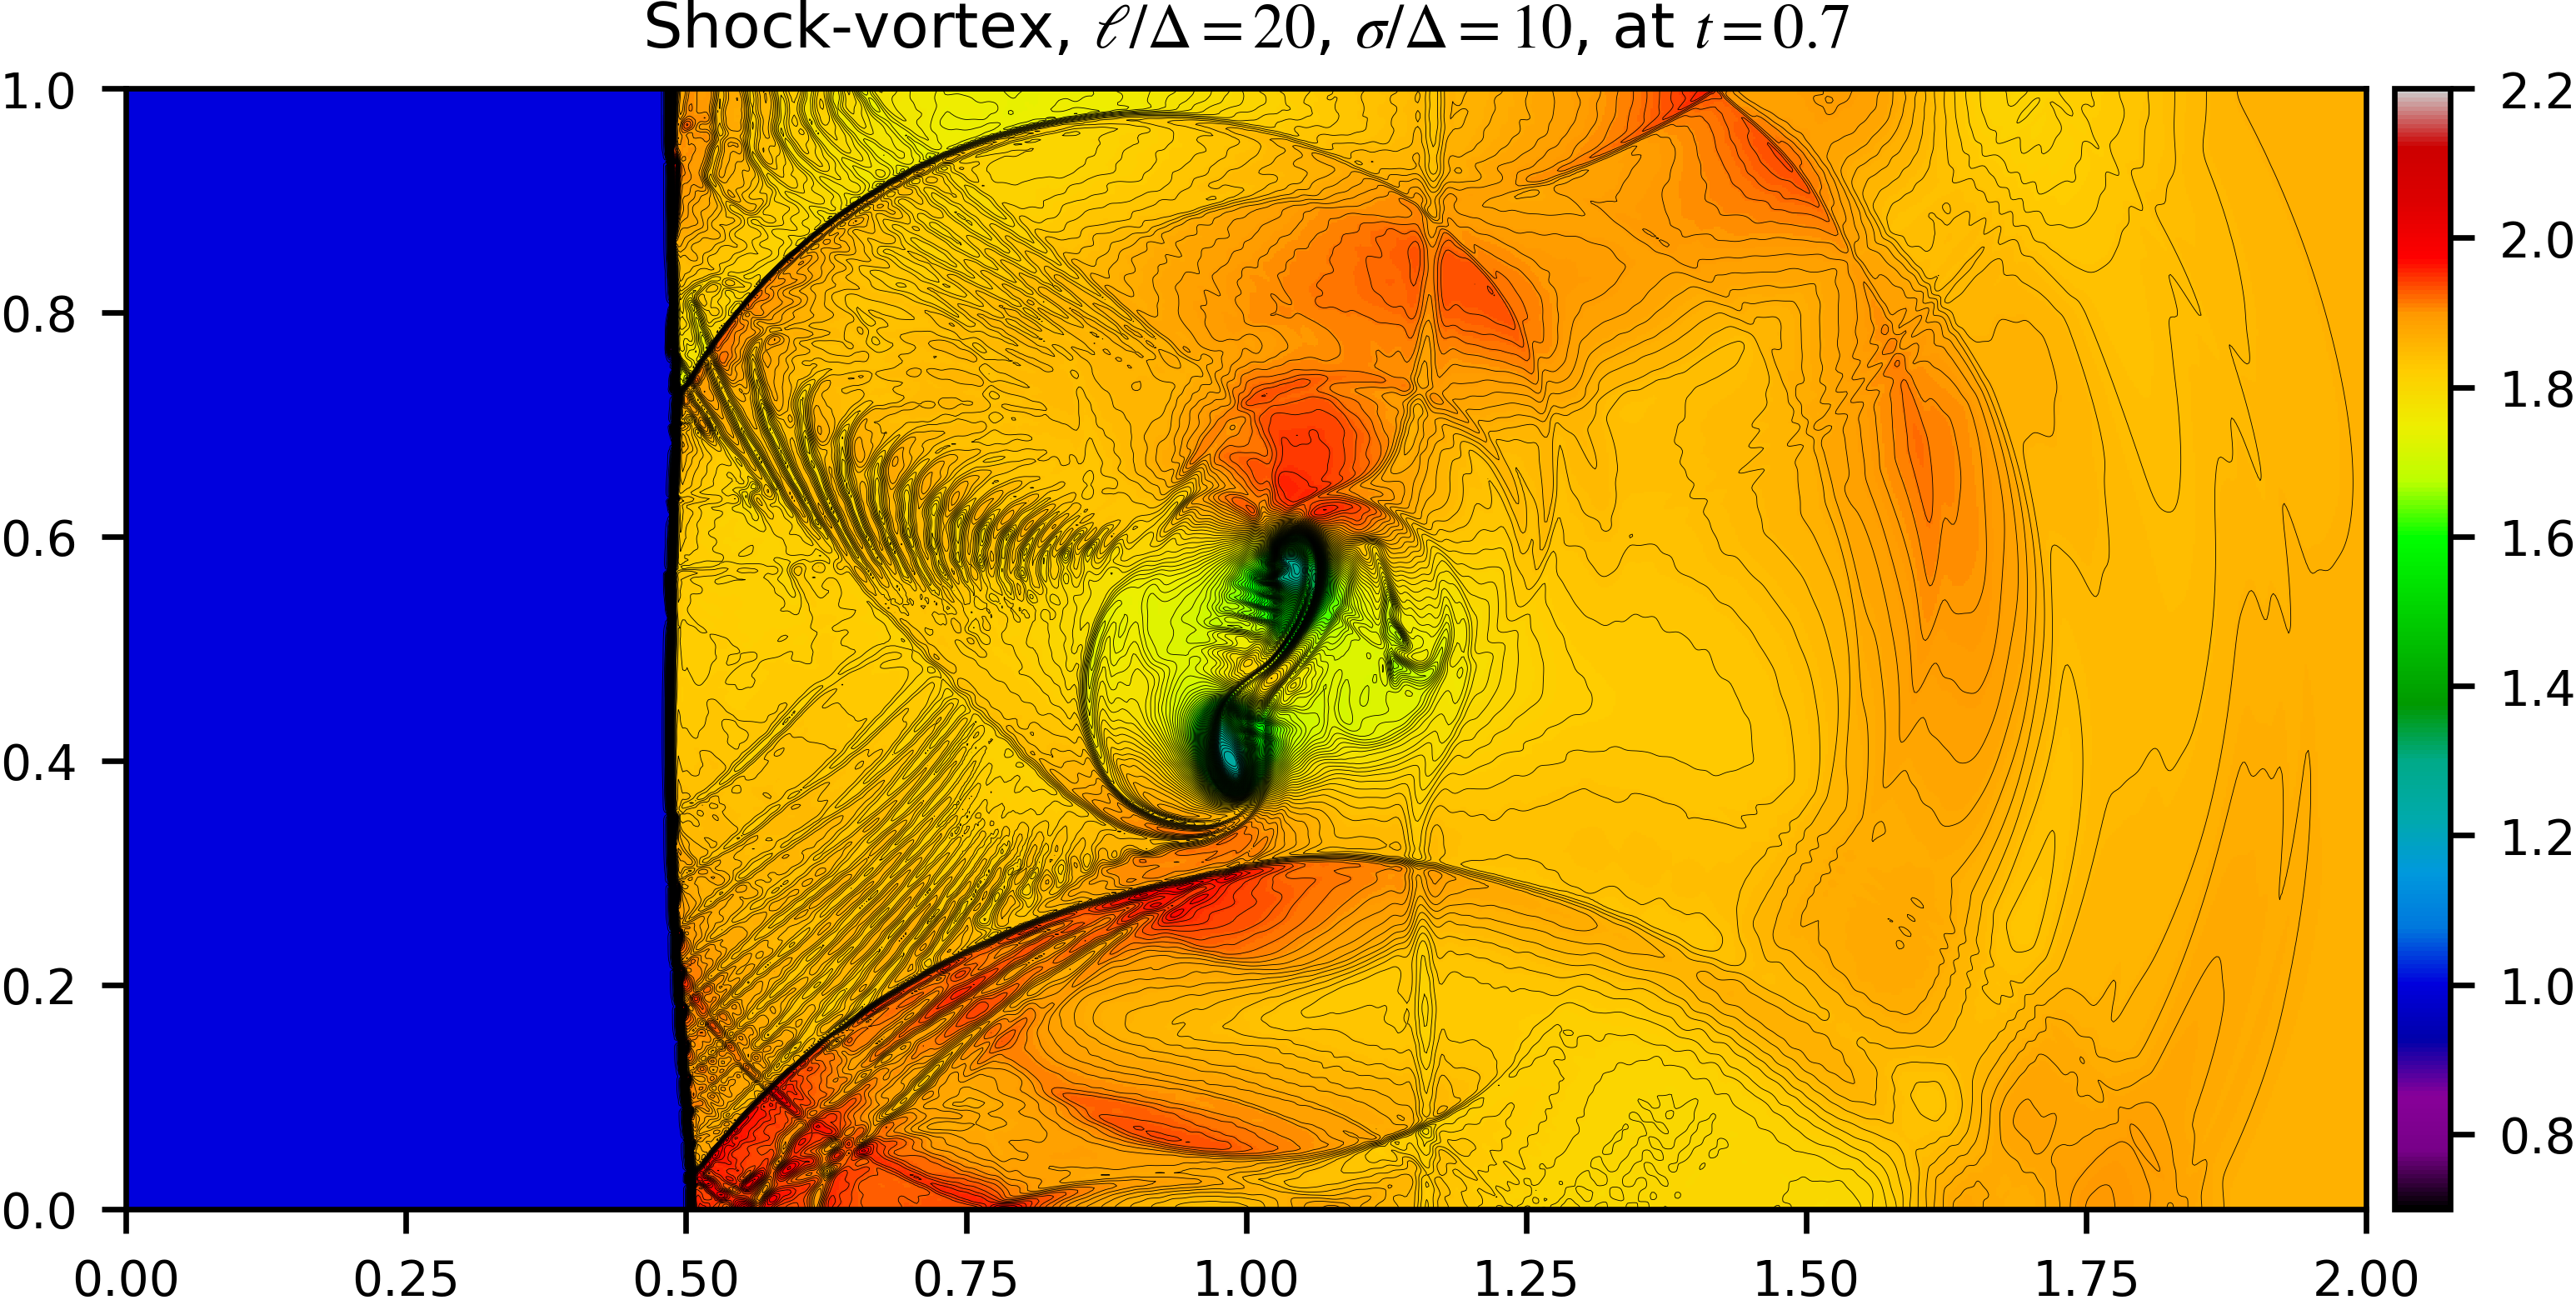
\includegraphics[width=0.95\textwidth]{fig/shockvortex_gp_ed20_sd10.png}
    \end{subfigure}
    \begin{subfigure}{120mm}
        \centering
        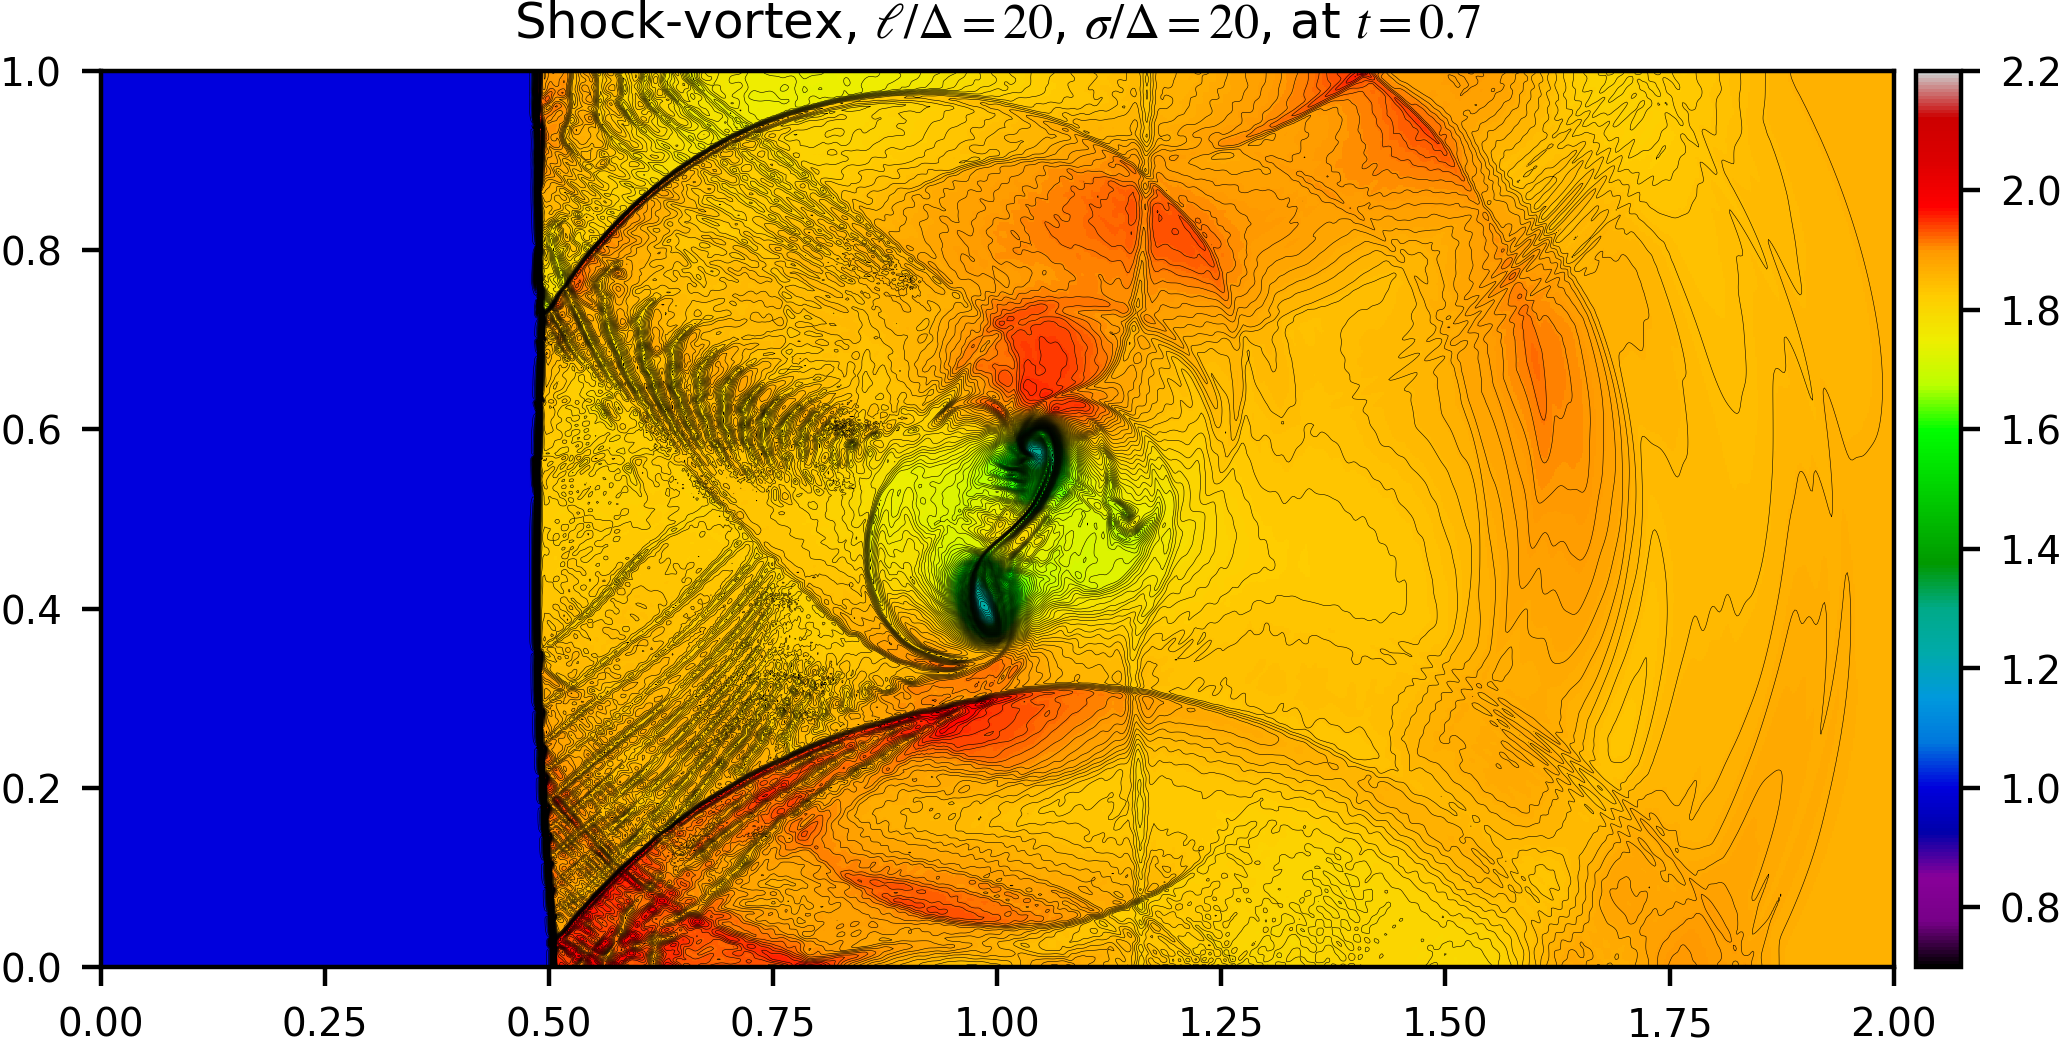
\includegraphics[width=0.95\textwidth]{fig/shockvortex_gp_ed20_sd20.png}
    \end{subfigure}
    \caption{The density colormaps of the strong shock vortex interaction problem.
        The GP-WENO (\( r = 2 \)) + SF-PIF3 method
        are used for all simulation runs
        on \( [1024 \times 512] \) grid resolution
        with varying hyperparameter, \( \sigma/\Delta \).
        The pseudo-colors represent the density map ranging between \( [0.75, 2.2] \),
        and 200 contour lines within the same range are over-plotted as solid black lines.
    }\label{fig:shockvortex}
\end{figure}

The results of the simulation of the GP-WENO method with varying \( \sigma \)
are presented in~\cref{fig:shockvortex}.
The SF-PIF3 method is used as a temporal method on a \( [1024 \times 512] \) grid resolution.
The obtained solutions with GP-WENO and SF-PIF3 methods are
well-comparable with the reference solution presented in~\cite{cheng2019two,galbraith5th}.
The GP hyperparameters are normalized with the grid scale \( \Delta \),
as suggested in~\cite{reyes2018new,reyes2019variable}.
The length-scale hyperparameters, \( \ell/\Delta = 20 \) is taken
based on the results of the previous section
(e.g., \( \ell/\Delta = 20 \) is equivalent to \( \ell = 1 \) with the vortex problem of \( 400 \times 400 \) resolution grid)
and various shock-capturing hyperparameters, \( \sigma/\Delta = 5, 10, \) and \( 20 \) are tested.

As shown in~\cref{fig:shockvortex}, the higher values of \( \sigma/\Delta \) is better
to capture the small-scale fluid structures, especially on the trailing waves of the vortex
around \( 0.5 \le x \le 1 \).
However, as discussed in~\cref{subsec:2drp_c3_weno} before,
identifying the numerical artifacts in the small-scale fluids is not feasible
without extensive numerical tests.
At a minimum, it is safe to say that the larger \( \sigma \) values
can produce less dissipative numerical solutions capturing the small-scale structures.


\label{ch:conclusion}

% \appendix % Uncomment if you have appendices. Add them below this exactly as you would a regular chapter.

\nocite{*}
\bibliographystyle{plain}
\singlespacing
\bibliography{dissertation}
\doublespacing

\end{document}
